\ifdefined\included
\else
\documentclass[a4paper,11pt,twoside]{StyleThese}
\usepackage{amsmath,amssymb}             % AMS Math
\usepackage[french]{babel}
\usepackage[utf8]{inputenc}
\usepackage[T1]{fontenc}
\usepackage{tabularx}
%\usepackage{tabular}
\usepackage{multirow}


\usepackage[tight,footnotesize]{subfigure}
\usepackage{algorithm} %To allow algorithm environment
\usepackage{algpseudocode} %Provides algorithmic environment

\usepackage{hhline}
\usepackage[left=1.5in,right=1.3in,top=1.1in,bottom=1.1in,includefoot,includehead,headheight=13.6pt]{geometry}
\renewcommand{\baselinestretch}{1.05}

% Table of contents for each chapter

\usepackage[nottoc, notlof, notlot]{tocbibind}
\usepackage[french]{minitoc}
\setcounter{minitocdepth}{2}
\mtcindent=15pt
% Use \minitoc where to put a table of contents

\usepackage{aecompl}

% Glossary / list of abbreviations

\usepackage[intoc]{nomencl}
\renewcommand{\nomname}{Liste des Abréviations}

\makenomenclature

% My pdf code

\usepackage{ifpdf}

\ifpdf
  \usepackage[pdftex]{graphicx}
  \DeclareGraphicsExtensions{.jpg}
  \usepackage[a4paper,pagebackref,hyperindex=true]{hyperref}
  \usepackage{tikz}
  \usetikzlibrary{arrows,shapes,calc}
\else
  \usepackage{graphicx}
  \DeclareGraphicsExtensions{.ps,.eps}
  \usepackage[a4paper,dvipdfm,pagebackref,hyperindex=true]{hyperref}
\fi

\graphicspath{{.}{images/}}

%nicer backref links
\renewcommand*{\backref}[1]{}
\renewcommand*{\backrefalt}[4]{%
\ifcase #1 %
(Non cité.)%
\or
(Cité en page~#2.)%
\else
(Cité en pages~#2.)%
\fi}
\renewcommand*{\backrefsep}{, }
\renewcommand*{\backreftwosep}{ et~}
\renewcommand*{\backreflastsep}{ et~}

% Links in pdf
\usepackage{color}
\definecolor{linkcol}{rgb}{0,0,0.4} 
\definecolor{citecol}{rgb}{0.5,0,0} 
\definecolor{linkcol}{rgb}{0,0,0} 
\definecolor{citecol}{rgb}{0,0,0}
% Change this to change the informations included in the pdf file

\hypersetup
{
bookmarksopen=true,
pdftitle="Évaluation de la sécurité des équipements grand public connectés à Internet",
pdfauthor="Yann BACHY", %auteur du document
pdfsubject="Thèse", %sujet du document
%pdftoolbar=false, %barre d'outils non visible
pdfmenubar=true, %barre de menu visible
pdfhighlight=/O, %effet d'un clic sur un lien hypertexte
colorlinks=true, %couleurs sur les liens hypertextes
pdfpagemode=None, %aucun mode de page
pdfpagelayout=SinglePage, %ouverture en simple page
pdffitwindow=true, %pages ouvertes entierement dans toute la fenetre
linkcolor=linkcol, %couleur des liens hypertextes internes
citecolor=citecol, %couleur des liens pour les citations
urlcolor=linkcol %couleur des liens pour les url
}

% definitions.
% -------------------

\setcounter{secnumdepth}{3}
\setcounter{tocdepth}{2}

% Some useful commands and shortcut for maths:  partial derivative and stuff

\newcommand{\pd}[2]{\frac{\partial #1}{\partial #2}}
\def\abs{\operatorname{abs}}
\def\argmax{\operatornamewithlimits{arg\,max}}
\def\argmin{\operatornamewithlimits{arg\,min}}
\def\diag{\operatorname{Diag}}
\newcommand{\eqRef}[1]{(\ref{#1})}

\usepackage{rotating}                    % Sideways of figures & tables
%\usepackage{bibunits}
%\usepackage[sectionbib]{chapterbib}          % Cross-reference package (Natural BiB)
%\usepackage{natbib}                  % Put References at the end of each chapter
                                         % Do not put 'sectionbib' option here.
                                         % Sectionbib option in 'natbib' will do.
\usepackage{fancyhdr}                    % Fancy Header and Footer

% \usepackage{txfonts}                     % Public Times New Roman text & math font
  
%%% Fancy Header %%%%%%%%%%%%%%%%%%%%%%%%%%%%%%%%%%%%%%%%%%%%%%%%%%%%%%%%%%%%%%%%%%
% Fancy Header Style Options

\pagestyle{fancy}                       % Sets fancy header and footer
\fancyfoot{}                            % Delete current footer settings

%\renewcommand{\chaptermark}[1]{         % Lower Case Chapter marker style
%  \markboth{\chaptername\ \thechapter.\ #1}}{}} %

%\renewcommand{\sectionmark}[1]{         % Lower case Section marker style
%  \markright{\thesection.\ #1}}         %

\fancyhead[LE,RO]{\bfseries\thepage}    % Page number (boldface) in left on even
% pages and right on odd pages
\fancyhead[RE]{\bfseries\nouppercase{\leftmark}}      % Chapter in the right on even pages
\fancyhead[LO]{\bfseries\nouppercase{\rightmark}}     % Section in the left on odd pages

\let\headruleORIG\headrule
\renewcommand{\headrule}{\color{black} \headruleORIG}
\renewcommand{\headrulewidth}{1.0pt}
\usepackage{colortbl}
\arrayrulecolor{black}

\fancypagestyle{plain}{
  \fancyhead{}
  \fancyfoot{}
  \renewcommand{\headrulewidth}{0pt}
}

%\usepackage{MyAlgorithm}
%\usepackage[noend]{MyAlgorithmic}
\usepackage[ED=MITT - STICIA, Ets=INP]{tlsflyleaf}
%%% Clear Header %%%%%%%%%%%%%%%%%%%%%%%%%%%%%%%%%%%%%%%%%%%%%%%%%%%%%%%%%%%%%%%%%%
% Clear Header Style on the Last Empty Odd pages
\makeatletter

\def\cleardoublepage{\clearpage\if@twoside \ifodd\c@page\else%
  \hbox{}%
  \thispagestyle{empty}%              % Empty header styles
  \newpage%
  \if@twocolumn\hbox{}\newpage\fi\fi\fi}

\makeatother
 
%%%%%%%%%%%%%%%%%%%%%%%%%%%%%%%%%%%%%%%%%%%%%%%%%%%%%%%%%%%%%%%%%%%%%%%%%%%%%%% 
% Prints your review date and 'Draft Version' (From Josullvn, CS, CMU)
\newcommand{\reviewtimetoday}[2]{\special{!userdict begin
    /bop-hook{gsave 20 710 translate 45 rotate 0.8 setgray
      /Times-Roman findfont 12 scalefont setfont 0 0   moveto (#1) show
      0 -12 moveto (#2) show grestore}def end}}
% You can turn on or off this option.
% \reviewtimetoday{\today}{Draft Version}
%%%%%%%%%%%%%%%%%%%%%%%%%%%%%%%%%%%%%%%%%%%%%%%%%%%%%%%%%%%%%%%%%%%%%%%%%%%%%%% 

\newenvironment{maxime}[1]
{
\vspace*{0cm}
\hfill
\begin{minipage}{0.5\textwidth}%
%\rule[0.5ex]{\textwidth}{0.1mm}\\%
\hrulefill $\:$ {\bf #1}\\
%\vspace*{-0.25cm}
\it 
}%
{%

\hrulefill
\vspace*{0.5cm}%
\end{minipage}
}

\let\minitocORIG\minitoc
\renewcommand{\minitoc}{\minitocORIG \vspace{1.5em}}

\usepackage{multirow}
%\usepackage{slashbox}

\newenvironment{bulletList}%
{ \begin{list}%
	{$\bullet$}%
	{\setlength{\labelwidth}{25pt}%
	 \setlength{\leftmargin}{30pt}%
	 \setlength{\itemsep}{\parsep}}}%
{ \end{list} }

\newtheorem{definition}{Définition}
\renewcommand{\epsilon}{\varepsilon}

% centered page environment

\newenvironment{vcenterpage}
{\newpage\vspace*{\fill}\thispagestyle{empty}\renewcommand{\headrulewidth}{0pt}}
{\vspace*{\fill}}

\usepackage{tablefootnote}
\sloppy
\begin{document}
\setcounter{chapter}{3} %% Numéro du chapitre précédent ;)
\dominitoc
\faketableofcontents
\fi

\chapter{Vers un Dialogue Situé Homme-Robot}
\label{chapter3}
\minitoc

\section{Contexte}

\subsection{Introduction}
%intro + related work
L'une des compétences essentielles pour interagir convenablement avec l'homme est de fournir des moyens d'assurer la compréhension mutuelle dans le contexte situé de l'activité jointe. Le robot et l'humain doivent avoir des références aux éléments de l'environnement qui soient communes (common ground), ce qui signifie qu'ils doivent pouvoir identifier, dans leur propre représentation du monde, les actions, les entités (humains, robots ou objets) et les propriétés énoncées par leur interlocuteur.
%TODO biblio on grounding / situated dialogue / reference generation

Les systèmes robotiques reposent sur les capteurs pour reconnaître et localiser les entités afin de construire l'état du monde. Ces capteurs produisent des coordonnées pour positionner les entités par rapport à un repère donné. Par exemple, une caméra stéréo avec un logiciel de reconnaissance peut permettre de savoir qu'une tasse est à une position donnée  $x$, $y$, $z$ avec une orientation $\theta$, $\phi$, $\psi$.
Les humains quand à eux, utilisent les relations spatiales entre les éléments pour décrire leur position. Pour indiquer la position de la tasse, l'humain dirait par exemple qu'elle se trouve sur la table de la cuisine, sans donner les coordonnées précises.
Pour comprendre les références de l'homme et générer des déclarations compréhensibles, le robot se doit donc de construire une représentation symbolique du monde, basée sur les données géométriques qu'il a collectées par ses capteurs, comme cela a été fait dans \cite{lemaignan2012grounding}.

%We have developed a module based on spatial and temporal reasoning to generate "facts" about the current state of the world \cite{milliez2014framework}. A fact is a property which describes the current state of an entity (e.g. $MUG$ $isNextTo$ $BOTTLE$, $MUG$ $isFull$ $TRUE$). This framework generates facts related to the entities' position and facts about affordances to know, for instance, what is visible or reachable to each agent (human and robot). 
%It also generates facts about agent postures to know if an agent is pointing toward an object or where an agent is looking. When the robot tries to understand the human, it should also use these data to improve the information grounding process.

En plus de l'état du monde (qui peut être considéré comme l'état de croyance du robot), pour vraiment comprendre les actes dialogiques de l'humain dans un contexte situé, il est nécessaire au robot de comprendre la situation spatiale et mentale de l'homme. En effet, les références qu'il crée dans ses actes communicatifs avec le robot sont susceptibles de grandement dépendre de cette situation spatiale ou mentale.

Pour établir ces références communes et comprendre les actes communicatifs humains à la lumière de sa situation, nous avons utilisé notre infrastructure logicielle d'évaluation de la situation, présentée dans les chapitres précédents, dans le cadre d'un projet visant à mettre en place un dialogue situé homme-robot


\subsection{Le projet MaRDi}
%Projet MaRDi (thèse Manu)
Ces travaux ont été réalisés dans le cadre du projet MaRDi\footnote{Man-Robot Dialogue - http ://mardi.metz.supelec.fr
} de l’Agence Nationale pour la Recherche (ANR). Il a été financé par l’appel à projet Contenu et interactions. Les
travaux réalisés ont été faits en collaboration avec le Laboratoire d’Informatique Fondamentale de Lille (LIFL), l’École supérieure d’électricité (Supélec), le groupe Acapela, le Laboratoire Informatique d’Avignon (LIA) et le Laboratoire d’Analyse et d’Architecture des Systèmes (LAAS).
Ce projet vise à étudier l’apport d’une approche "située" du dialogue homme-robot. Le terme "située" est ici relatif à l’incarnation physique d’un système de dialogue dans une plateforme robotique qui permet l’intégration d’informations issues de la perception du robot dans le contexte de l’interaction pour compléter ou lever des ambiguïtés introduites par le médium vocal. Ce projet s’inscrit également dans l’utilisation de méthodes d’apprentissage numérique, exploitant les données collectées au travers de la conduite de véritables interactions afin d’améliorer l’efficacité et le naturel du système dans le temps. L’originalité de l’approche est de ne pas considérer les technologies vocales comme disponibles et dissociées de la tâche d’interaction homme-robot, mais bel et bien comme moyen d’en améliorer l’expérience et les performances.

En effet, le système de dialogue utilisé dans le cadre de ce projet est basé sur le système de résolution de la tâche \textit{TownInfo} qui vise à fournir aux utilisateurs un service vocal donnant accès à des
informations touristiques concernant une ville virtuelle et portant essentiellement sur la
recherche de données pratiques (téléphone, adresse, etc.) sur des établissements (hôtels,
restaurants, bars et infrastructures). Il s'agit donc d'un système de dialogue de type recherche d'informations pour s'enquérir des choix de l'utilisateur (e.g: restaurant chinois à cinq minutes) et pouvoir lui proposer les établissements correspondant au mieux à cette demande. 
Nous utilisons une implémentation
du système de dialogue basée sur celle proposée par l’université de Cambridge et qui repose
sur le formalisme POMDP-HIS \cite{Young10}.
L'une des caractéristiques de ces systèmes est qu'ils peuvent également effectuer une relâche de contrainte pour proposer une solution proche des critères de l'utilisateur si aucune solution n'a été trouvée.

La tâche MaRDi ne peut cependant pas être directement
assimilable à un problème de recherche d’information standard.
Pour donner l'aspect incorporé, le robot doit être capable de maintenir un contexte d’interaction suffisamment riche pour pouvoir être à même de prendre des décisions sur la suite à donner à celle-ci. Ce contexte intègre les entrées fournies par l’humain mais aussi les informations issues des calculs géométriques et des raisonnements effectués à partir de la perception de l’environnement. Sur ces aspects en particulier,
le projet s'appuie sur les recherches présentées aux chapitres précédents, pour le raisonnement
spatial et la prise de perspective, pour tenter de résoudre des ambiguïtés.
Pour prendre des décisions afin de poursuivre l’interaction, la machine devra s’appuyer sur un contexte de l’interaction (historique, état de l’environnement, etc.) et tenir
compte de son aspect incertain. En effet, dans le cadre situé, le contexte de l’interaction ne peut être considéré comme une donnée sûre car de possibles erreurs ont pu être
introduites par la chaîne de traitement automatique des entrées vocales et visuelles.
%C’est pourquoi les approches stochastiques que nous employons nous permettent de
%modéliser les différentes hypothèses avec leur score de confiance respectif. Ainsi, la
%stratégie d’interaction employée par la machine devra tenir compte des ambiguïtés potentiellement générées et en garder trace tout au long du dialogue. Nous traiterons
%cette problématique par l’utilisation de modèles permettant l’optimisation statistique
%du mécanisme de prise de décision. La faculté d’adaptation à un nouveau profil utilisateur ou plus généralement à des situations contextuelles et dialogiques différentes
%lors de l’apprentissage est une caractéristique désirée qui fera également l’objet de nos
%travaux.
Une fois sa décision prise, le système devra également pouvoir la restituer vocalement et physiquement à l’humain. Ainsi il faudra qu’il soit capable de planifier ses
mouvements et ses actions physiques de façon précise pour répondre aux besoins de
l’utilisateur (déplacer un objet, se rendre dans une pièce, etc.), mais également capable
de s’exprimer de façon adéquate pour se faire comprendre par l’utilisateur et lui témoigner de sa compréhension du contexte interactif courant. Pour cela, le robot devra par
exemple adopter des attitudes physiques particulières, ou encore utiliser une intonation de
voix particulière.


\subsection{Scénario associé}

Afin de positionner le scénario dans un cadre naturel et fonctionnel, le choix a été
fait de faire interagir un robot assistant avec une personne handicapée dans son appartement (aide
à la personne). La personne pourra ainsi, en interagissant avec le robot, lui faire manipuler divers objets. Les objets en question auront des propriétés associées en terme de couleur, de type d'objet (par exemple un DVD), de type de contenu (par exemple science-fiction) et de position et auront un identifiant unique. Pour se faire comprendre
par le robot, l’utilisateur usera principalement de la parole, mais pourra également employer des gestes déictiques (comme le fait de pointer un objet particulier).
Un dialogue multimodal sera ici employé pour pouvoir résoudre les possibles ambiguïtés liées à une précision insuffisante de la requête utilisateur.
Ce dialogue se poursuivra jusqu’à la fin de l’exécution effective de la tâche ou
l’échec de l’interaction. Cette dernière situation peut par exemple être due à un désengagement explicite de l’utilisateur, ou encore à l’exécution d’une commande erronée
de la part du robot. Un exemple d’un tel dialogue multimodal est donné dans le tableau \ref{table:dial}.
Dans ce contexte d’étude nous pourrons également jouer sur la définition de divers
scénarios (configuration de l’environnement, connaissances initiales du robot, position
des agents, etc.) pour rendre l’interaction plus ou moins complexe. Ceci nous permet de
pouvoir tester divers cas d’interactions, notamment dans des configurations "limites" comme celles employées lorsque nous étudierons les tâches de fausse croyance (voir \ref{sec:mentalStateDial}).



\begin{table}
\centering
\small
\begin{tabular}{|c|l|}
  \hline
  \multirow{2}{*}{Robot1} & Comment Puis-je vous aider? \\
    & hello() [Greet] \\
    \hline
  \multirow{2}{*}{User1}  & Peux-tu mettre le livre sur ma table de chevet? \\
  	& inform(cmd.action=move, cmd.location=bedroom\_bedsidetable) \\
    \hline
  \multirow{2}{*}{Robot2} & Désolé, mais savez vous où se trouve le livre dont vous me parlez? \\
    & confreq(object.type=book,object.location) [TentRQ] \\
    \hline
  \multirow{2}{*}{User2} & C’est celui là. \\
  	& inform(idobj= ?) + pointsAt BLUE\_BOOK = inform(idobj=BLUE\_BOOK) \\
   \hline
    \multirow{5}{*}{Robot3} & Ok, je vais mettre le livre bleu sur votre table de chevet. \\
     & execute(cmd.action=move,cmd.location=bedroom\_bedsidetable, \\
     & idobj=BLUE\_BOOK,object.location=livingroom\_table,object.type=book, \\
     & object.color=blue) [Execute] \\
     & move(BLUE\_BOOK,livingroom\_table,bedroom\_bedsidetable) \\
    \hline
\end{tabular}
 \caption{Exemple de dialogue multimodal.}
 \label{table:dial}
% \vspace{-20pt}
 \end{table}


% Robot1 >
% Usr1 >
% Robot2 >
% Usr2 >
% Robot3 >
% Comment puis-je vous aider ?
% hello() [Greet]
% Peux-tu mettre le livre sur ma table de chevet ?
% inform(cmd.action=move, cmd.location=bedroom_bedsidetable)
% Désolé, mais où se trouve le livre dont vous me parlez ?
% confreq(object.type=book,object.location) [TentRQ]
% C’est celui là
% inform(idobj= ?) + pointsAt BLUE_BOOK = inform(idobj=BLUE_BOOK)
% Ok, je vais mettre le livre bleu sur votre table de chevet
% execute(cmd.action=move,cmd.location=bedroom_bedsidetable,
% idobj=BLUE_BOOK,object.location=livingroom_table,object.type=book,
% object.color=blue) [Execute]
% move(BLUE_BOOK,livingroom_table,bedroom_bedsidetable)



% \begin{table}
% \centering
% \small
% \begin{tabular}{|c|c|l|}
%   \hline
%   \multirow{3}{*}{R1} & DA & hello() \\
%     & NLG/TTS & Can I help you ?\\
%     \hline
%   \multirow{3}{*}{U1} & ASR & Can you put the book in my bedroom? \\
%   	& SLU & inform(action=move,desc=in,room=bedroom)\\
%     \hline
%   \multirow{3}{*}{R2} & DA & confreq(type=book,position) \\
%     & NLG/TTS & Sorry but where is the book you are talking about?\\
%     \hline
%   \multirow{3}{*}{U3} & ASR & I am talking about this one \\
%   	& SLU & inform(idobj=?)\\
%     & GRU & pointsAt BLUE\_BOOK 1395848705.31\\
%    \hline
%     \multirow{4}{*}{R3} & & execute(action=move,destination=bedroom\_bedsidetable,\\
%      & DA & idobj=BLUE\_BOOK,position=livingroom\_table,type=book,\\
%     & &color=blue) \\
%     & NVBP/MC & move(BLUE\_BOOK,livingroom\_table,bedroom\_bedsidetable)\\
%     & NLG/TTS & Ok, I will put the blue book on your bedside table\\
%     \hline
% \end{tabular}
%  \caption{Example of a multimodal dialogue.}
%  \label{table:hri-example}
%  \vspace{-20pt}
%  \end{table}


Le robot utilisé est le PR2. L'appartement choisi pour conduire nos expériences est la réplique taille réelle
d’un 3 pièces (salon, cuisine, chambre) présent dans les locaux du LAAS-CNRS et dont une modélisation fidèle a été faite sur simulateur 3D.
Dans chaque pièce se trouvent des meubles, sur lesquels des objets peuvent être posés. Une version tridimensionnelle de cet environnement est représenté à la figure \ref{fig:env}.







\begin{figure}[ht!]
 \centering
  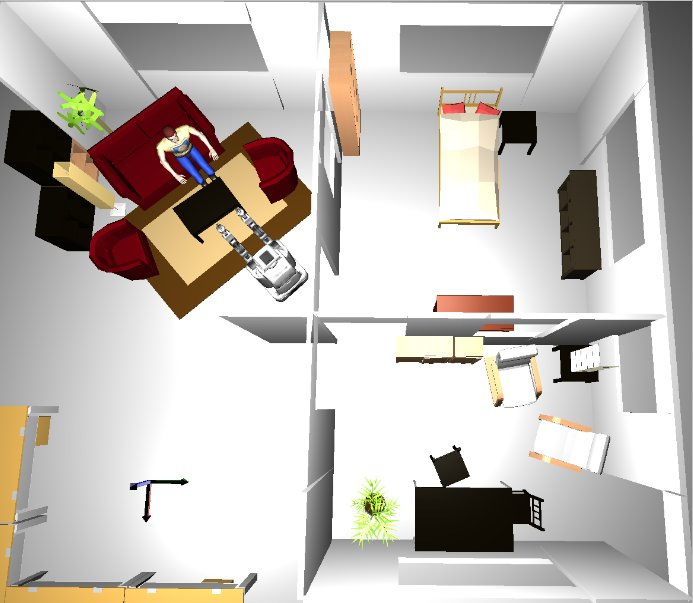
\includegraphics[width=0.89\linewidth]{./img/mardiSetup.jpg} 
  \caption {Représentation tridimensionnelle de l'environnement utilisé dans le cadre du projet MaRDi.}
  \label{fig:env}
\end{figure}




%%%%%%%%%%%%%%%%%%%%%%%%%%%%%%%%%%%%%%%%%%%%%%%%%%%%%%%%%%%

\section{Les trois phases de l'interaction}
\label{sec:troisPhases}



L'architecture mise en place pour la réalisation de l'interaction contient divers modules qui interviennent à différentes étapes.
Pour plus de clarté, nous distinguons trois phases de l'interaction permettant d'aller de la détermination du but utilisateur à son accomplissement. 

\begin{itemize}
\item La première phase fait intervenir les éléments permettant le bon fonctionnement du dialogue situé afin de communiquer avec l'utilisateur pour pouvoir le satisfaire (en lui procurant une information ou en agissant sur l'environnement).
\item La deuxième phase consiste à transmettre un but au planificateur afin que celui-ci puisse, en utilisant les informations sur la configuration actuelle de l'environnement, trouver un plan qui permette d'atteindre le but. Ce but peut être issu d'une demande explicite de l'utilisateur (e.g. \textit{"apporte moi le DVD du Seigneur des Anneaux"}) ou d'un but "intermédiaire" afin que le robot puisse acquérir une information manquante sur l'environnement.
\item La dernière phase fait intervenir la supervision qui pilote la planification de trajectoires et de mouvements et contrôle le bon déroulement de l'exécution de la tâche à accomplir.
\end{itemize}

Ces différentes phases font intervenir divers éléments du système. Durant une interaction les différentes phases sont utilisées à divers moments pour pouvoir faire progresser l'interaction.
Ainsi, selon ce que veut l'utilisateur certaines phases peuvent être appelées plusieurs fois ou pas du tout.
En effet, dans le cas le plus simple où l'utilisateur demande une information au robot et que celui-ci a déjà cette information, seule la première phase sera utilisée alors que sur des scénarios plus complexes, le système va boucler plusieurs fois en passant par les différentes phases avant de pouvoir satisfaire la demande de l'utilisateur.
Nous allons détailler les processus impliqués dans chaque phase et les échanges de données.

\subsection{Détermination de la demande utilisateur}
\label{sec:phase1}
Durant cette phase, l'humain et le robot dialoguent et le système essaye de caractériser la demande de l'utilisateur. Pour expliquer les différents flux, nous nous appuierons sur la figure \ref{fig:phase1}.


\begin{figure}[ht!]
 \centering
  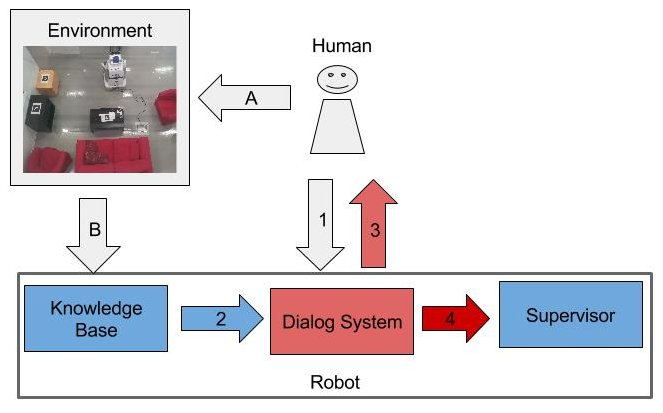
\includegraphics[width=0.99\linewidth]{./img/phase1color.jpg} 
  \caption {Schéma des différents composants et flux intervenant dans la phase de détermination du but utilisateur.}
  \label{fig:phase1}
\end{figure}

Dans cette première phase, l'homme peut en permanence agir sur l'environnement (flux A). L'environnement étant en permanence mis à jour par notre système d'évaluation de la situation (B), la base de connaissance sera mise à jour en conséquence.
Lors de cette phase d'estimation de la demande de l'utilisateur, l'homme parle au robot (1) en utilisant potentiellement des signes pour accompagner sa parole. Le système de dialogue du robot interprète l'acte communicatif de l'homme en utilisant sa base de connaissances (2) et produit une réponse appropriée à l'homme, par exemple en lui demandant une précision sur la tâche à accomplir (3). L'opération est répétée (flux 1, 2, 3) jusqu'à ce que le système de dialogue ait une compréhension suffisante de ce que veut l'homme. Si le système de dialogue peut répondre à la demande il le fait et attend la prochaine tâche. Cependant, dans le cas où le système robotique doit agir pour acquérir une information ou pour apporter des modifications à l'environnement, à la place de répondre à l'homme (3) le système de dialogue envoie un but au superviseur (4). La première phase est alors interrompue et l'interaction passe dans la phase d'élaboration de plan permettant de résoudre le but (qui peut être directement un but provenant de l'utilisateur ou un but intermédiaire permettant l'acquisition d'informations).

\subsection{Élaboration de plan}
\label{sec:phase2}
Durant cette phase, le robot cherche à générer un plan permettant de résoudre le but produit lors de la première phase. Pour expliquer les différents flux, nous nous appuierons sur la figure \ref{fig:phase2}.

\begin{figure}[ht!]
 \centering
  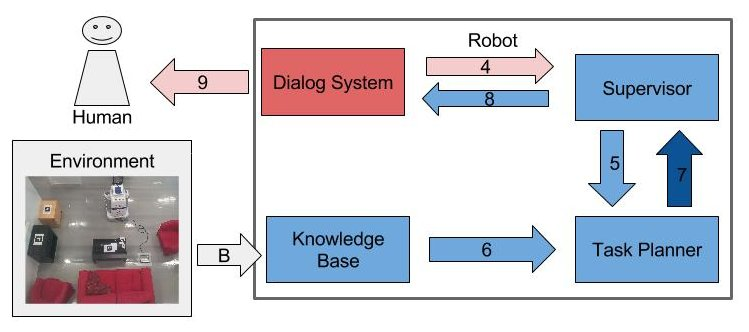
\includegraphics[width=0.99\linewidth]{./img/phase2color.jpg} 
  \caption {Schéma des différents composants et flux intervenant dans la phase d'élaboration de plan pour résoudre un but.}
  \label{fig:phase2}
\end{figure}

À la fin de la première phase, lorsque un but est produit, le système de dialogue transmet le but au superviseur (flux 4). Le superviseur par la suite fait une requête au planificateur de tâches pour résoudre le but (5). Le planificateur de tâche utilise la représentation symbolique de l'environnement, contenu dans la base de connaissance et provenant des calculs et raisonnements faits par le système d'évaluation de la situation, pour avoir connaissance de l'état du monde actuel et générer un plan permettant d'atteindre le but souhaité par l'utilisateur. Le planificateur de tâche renvoie un message au superviseur lui informant du succès ou de l'échec de la planification (7). En cas d'échec, le superviseur informe le système de dialogue (8) qui à son tour informe l'humain de l'impossibilité d'exécution du plan (9).
L'interaction retourne alors à la phase précédente afin de tenter d'établir un but utilisateur qui soit réalisable. 
Dans le cas où la planification est un succès (un plan a été trouvé), le plan est envoyé au superviseur (7) et l'interaction peut passer à la phase d'exécution du plan.


\subsection{Exécution du plan}
\label{sec:phase3}
Durant cette phase, le robot cherche à exécuter les tâches du plan permettant d'accomplir le but. Pour expliquer les différents flux, nous nous appuierons sur la figure \ref{fig:phase3}.




\begin{figure}[ht!]
 \centering
  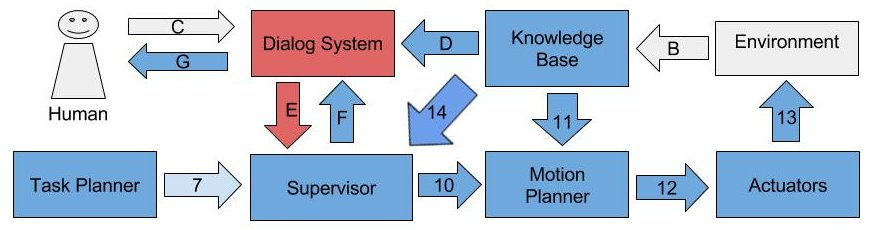
\includegraphics[width=0.99\linewidth]{./img/phase3color.jpg} 
  \caption {Schéma des différents composants et flux intervenant dans la phase d'exécution de plan pour accomplir le but utilisateur.}
  \label{fig:phase3}
\end{figure}

À la fin de la phase précédente, le planificateur de tâche transmet le plan à la supervision (flux 7). Le composant de supervision gère l'exécution de la tâche grâce à la planification de mouvements (10) qui envoie des commandes aux actionneurs du robot (12). Le superviseur contrôle la bonne exécution du plan à l'aide des éventuels retours d'erreurs des différents composants et en surveillant l'évolution de l'état du monde (14). Durant cette exécution, l'homme peut à tout moment dialoguer avec le système (C) afin de:
\begin{itemize}
\item Demander une information sur l'environnement. Dans ce cas le système de dialogue utilise la base de connaissance (D) pour répondre au mieux à l'humain (G).
\item S'enquérir de l'état d'avancement de la tâche ou de l'action courante du robot. Dans ce cas le système de dialogue envoie une requête correspondante au superviseur (E) qui transmet cette information à l'homme (G) par le système de dialogue (F).
\item Demander un abandon de la tâche ou un changement de plan. Le système de dialogue transmet alors cette requête au superviseur (flux E). Puis en cas d'abandon, l'interaction retourne en phase de détermination de but utilisateur ou en cas de changement de plan, en phase d'élaboration d'un nouveau plan prenant en compte les demandes de l'utilisateur. Cette dernière fonctionnalité est présentée plus en détail en section \ref{sec:planning}.
\end{itemize}

%mais ne sont pas nécéssairement séquencées de façon ordonée. En effet, durant la phase d'identification du but utilisateur, il est possible qu'un but "intermédiaire" soit généré par le robot afin de faire avancer le dialogue et l'identification du but final de l'utilisateur. Par exemple, le robot peux décider d'aller verifier un fait en se déplaçant dans l'appartement, soulevé une boîte pour montrer à l'homme ce qu'il s'y trouve... Il est donc possible que le robot ait à planifier ou à agir pour mettre à jour son état de connaissance de l'environnement ou celui de l'homme.
%De même, durant la phase de planification, il est possible de faire intervenir le dialogue pour négocier le plan, demander des conseils à l'homme ou l'informer de l'échec de la planification.
%Enfin, durant l'execution, il est nécéssaire que le robot informe l'homme de l'évolution de la tâche. Le robot doit également pouvoir proposer une alternative au but de l'homme si le but donné par l'homme n'est pas atteignable.
%Pour améliorer l'intéraction, l'homme devrait également pouvoir demander des informations au robot ou lui demander d'abandonner la tâche pendant l'execution.




\section{Architecture du système de dialogue situé}

Dans cette partie, nous allons aller plus loin dans l'explication du système de dialogue situé, intervenant principalement dans la première phase, en détaillant les différents modules qui entrent en jeu lors de la détermination du but utilisateur. Nous allons notamment détailler comment le système de dialogue est enrichi en utilisant le contexte de l'interaction et la base de faits maintenue par le système d'évaluation de la situation.

Nous considérons ici une interaction pouvant être modélisée par une alternance de "tours" entre les deux participants. Cet enchaînement de tours est appelé cycle du dialogue. Un tour représente le laps de temps pendant lequel un des participants peut s’adresser à l’autre pour faire progresser le dialogue.

La plupart des travaux sur les systèmes de dialogue \cite{Levin97,Young10,thomson2010bayesian} utilisent une architecture incorporant:
\begin{itemize}
\item Des modules de compréhension pour interpréter la parole générée par l'interlocuteur.
\item Un gestionnaire de dialogue lié à une base de données afin de prendre une décision pour continuer l'interaction.
\item Des modules de générations permettant de restituer la décision à l'interlocuteur.
\end{itemize}
Ce type d'architecture est illustré par la figure \ref{fig:archidial}.

\begin{figure}[ht!]
 \centering
  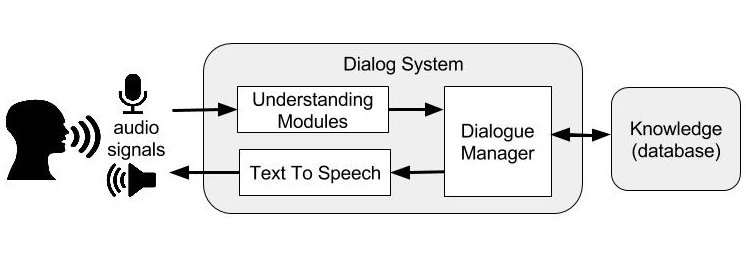
\includegraphics[width=0.99\linewidth]{./img/dialogueSys.jpg} 
  \caption {Architecture usuelle d'un système de dialogue.}
  \label{fig:archidial}
\end{figure}


Notre système de dialogue a la particularité d'être un système multimodal, c'est à dire dans lequel la gestuelle et la parole sont utilisés, et situé, c'est à dire que le contexte physique de l'interaction doit être pris en compte. Nous avons donc incorporé dans les entrées du système le contexte produit par TOASTER.
Nous présentons à la figure \ref{fig:archiphase1}, l'architecture détaillée mise en place pour permettre la communication avec l'utilisateur. Nous nous baserons sur cette figure pour expliquer les différents flux, ainsi que les différents modules qui permettent le bon fonctionnement du dialogue situé. Cette architecture est issue de la collaboration du LIA et du LAAS-CNRS et est également présentée dans la thèse d'Emmanuel Ferreira dans \cite{ferreira2015phd}.


\begin{figure}[ht!]
 \centering
  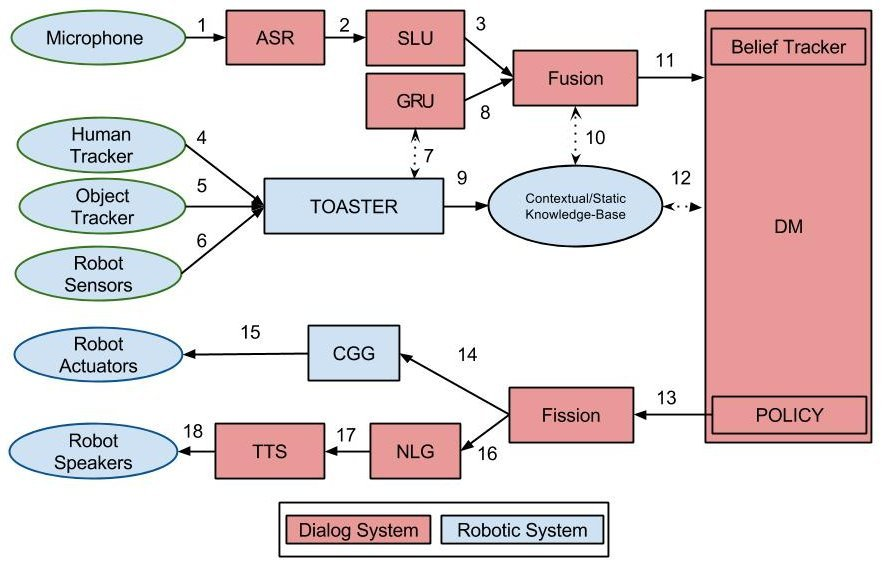
\includegraphics[width=0.99\linewidth]{./img/archiphase1.jpg} 
  \caption {Architecture détaillant les différents composants du système de dialogue situé élaborée pour le projet MaRDi.}
  \label{fig:archiphase1}
\end{figure}

Il est possible d'identifier plusieurs sous parties dans cette architecture.
La première est en charge des entrées multimodales de l'utilisateur. Une deuxième partie est responsable de l'acquisition et du maintien de l'état du monde ainsi que de la génération de données symboliques. Le gestionnaire de dialogue, ou DM (Dialogue Manager) permet de décider, en fonction des entrées interprétées de l'utilisateur et du contexte de l'interaction de la réponse donnée par le robot afin de parvenir à qualifier la demande de l'utilisateur.
La dernière partie s'attache à restituer sous forme multimodale la sortie du système de dialogue décidée par le gestionnaire de dialogue.
Certains modules relevant d'avantage du dialogue proprement parlé que de l'usage du système d'évaluation de la situation, une description brève en sera donnée. Pour plus de renseignements sur ces modules et une description plus exhaustive de la partie dialogue, nous invitons le lecteur à consulter les articles \cite{Ferreira13a,Ferreira13b} ainsi que la thèse \cite{ferreira2015phd}.

\subsection{Entrées multimodales utilisateur}
\label{sec:entréesDial}
Cette première partie permet d'acquérir et d'interpréter les entrées multimodales de l'homme en fonction du contexte de l'interaction. L’utilisateur peut faire l’usage de la parole et/ou de gestes déictiques de façon non contrainte tout au long de l’interaction pour s’adresser au robot. Une fois la commande de l'utilisateur interprétée, elle est transmise au module de gestion de dialogue. 

Pour acquérir et interpréter les commandes de l'utilisateur, quatre modules sont impliqués.

\begin{itemize}
\item \textbf{Le module \textit{ASR}}: la reconnaissance de la parole est effectuée grâce au module \textit{ASR} (Automatic Speech Recognition). Il utilise le flux audio (flux 1 sur le schéma) provenant du microphone pour traduire ce flux en mots. Ce module est basé sur la Google Web Speech API 3.

\item \textbf{Le module \textit{SLU}}: l'\textit{ASR} fournit les mots possiblement prononcés par l'homme au \textit{SLU} (2). Ces mots sont interprétés par le \textit{SLU} (Spoken Language Understanding) pour permettre de relier les mots aux concepts mis en jeux.

\item \textbf{Le module \textit{GRU}}: ce module est chargé de la reconnaissance et la compréhension des gestes déictiques émis par l’utilisateur lors de son tour d’interaction (Gesture Recognition and Understanding). Les gestes de pointage sont détectés et interprétés dynamiquement par notre raisonneur spatial (\textit{TOASTER}) décrit au chapitre \ref{chapter1} de cette thèse. Ce dernier exploite à la fois les coordonnées spatiales des objets (5) et les jointures de l’utilisateur (4) telles que déterminées grâce aux informations issues des capteurs visuels du robot pour savoir si un objet est pointé par l’utilisateur. Lorsque c’est le cas, un \textit{fait} de la forme \textit{AGENT\_ID pointsAt
OBJECT\_ID} est alors généré et transmis au GRU (7). De plus, ce \textit{fait}, comme tous les faits générés par notre infrastructure de raisonnement géométrique, contient un indicateur temporel. Cela permet de simplifier le mécanisme de
fusion avec les entrées vocales.
Bien que les composants aient été prévu pour s'interfacer de la façon décrite, dans le cadre du projet MaRDi le lien (7) n'a pas pu être établi, par manque de temps, lors de l'intégration du système.

%Dans la version actuelle de la plateforme des heuristiques expertes sont employées pour la capture de ces gestes dans SPARK. Cependant, une fois que plus de données auront été collectées, des techniques plus élaborées pourront être envisagées pour les remplacer, comme par exemple celle proposée dans (Rossi et al., 2013) qui fait intervenir un classifieur HMM avec en entrée des données issues d’une caméra RGB-D (coordonnées 3D et angles des jointures du corps de l’utilisateur, état ouvert/fermé de chacune de ses mains, etc.).

\item \textbf{Le module de fusion}: l’objectif du mécanisme de fusion est de combiner les actes de dialogue extraits du
signal de parole utilisateur (3) aux événements déictiques capturés grâce au module \textit{GRU} (8).
Pour ce faire, il faut tenir compte à la fois du contexte de l’interaction (positions des objets dans l’environnement physique, etc.), du niveau de confiance que l’on porte aux différentes hypothèses unimodales (étant donné qu’elles peuvent être erronées) mais également à leur marqueur temporel.
La première étape de ce processus consiste donc à déterminer si les hypothèses en
provenance des différentes modalités sont synchrones entre elles et peuvent être fusionnées ou doivent être considérées séparément. Du fait que la parole est considérée dans notre étude comme modalité principale de l’utilisateur, les tours d’interaction seront calés sur celui des entrées vocales. Ainsi, comme dans \cite{Holzapfel2004}, seuls les gestes déictiques détectés dans un segment temporel de 20ms avant et après celui du tour de parole courant seront exploités par le mécanisme de fusion. De ce fait, si des entrées \textit{SLU} apparaissent seules ou que les gestes détectés ne leur sont pas synchrones, elles seront directement considérées comme résultat de la fusion. La méthode de fusion retenue ici repose sur la définition d’un ensemble
de règles.
Par exemple si l’utilisateur prononce la
phrase « prends ça » tout en désignant un objet du doigt la fusion a pour rôle principal d’identifier un candidat valable. Pour ce faire le mécanisme de fusion s’appuie notamment sur la détection de concepts bas niveau qui témoignent d’un besoin de résolution de référents dans l’énoncé utilisateur (le mot « ça » dans l’exemple précédent).

La dernière étape du processus consiste à convertir les hypothèses ainsi produites
dans leur représentation sémantique haut niveau pour pouvoir les transmettre au gestionnaire de dialogue (11).
Des heuristiques définies manuellement sont employées pour déterminer les valeurs
des concepts de haut niveau identifiés à partir des hypothèses bas niveau.
\end{itemize}

Pour illustrer les mécanismes de compréhension des entrées utilisateur, un exemple de phrase utilisateur et de son interprétation par le système est donné au tableau \ref{table:fusion}.

% Phrase utilisateur
% Sémantique
% bas niveau
% Regroupement
% Sémantique
% haut niveau
% Passe moi le livre bleu qui est sur la table du salon
% inform(action=give, type=book, color=blue,
% spatial.indicator=on, type=table, room=livingroom)
% inform(cmd.action=give, object.type=book, object.color=blue
% object.location=[spatial.indicator=on, type=table,
% room=livingroom])
% inform(cmd.action=give, object.type=book, object.color=blue,
% object.position=livingroom\_table)
% TABLE 6.4 – Exemple d’extraction sémantique complète de la tâche MaRDi.

\begin{table}
 %\vspace{-10pt}
\centering
\renewcommand{\arraystretch}{1.3}
\begin{tabular}{|c|c|}
\hline
  \textbf{Phrase utilisateur} & Passe moi le livre bleu qui est sur la table du salon. \\
  \hline
  \textbf{Sémantique} & inform(action=give, type=book, color=blue, \\
  \textbf{bas niveau} & spatial.indicator=on, type=table, room=livingroom) \\
  \hline
 \textbf{Regroupement} & inform(cmd.action=give, object.type=book, \\
      & object.color=blue, object.location=[spatial.indicator=on, \\
      & type=table, room=livingroom]) \\
  \hline
  \textbf{Sémantique} & inform(cmd.action=give, object.type=book, \\
  \textbf{haut niveau} & object.color=blue, object.position=livingroom\_table) \\
  \hline
\end{tabular}
\caption{Exemple de phrase utilisateur et de l'interprétation qui en est faite par le système.}
%    \vspace{-10pt}
 \label{table:fusion}
 \end{table}


% \subsection{Entrées Multimodales de l'Utilisateur}

% Dans notre contexte applicatif, l’utilisateur peut faire l’usage de la parole et/ou de
% gestes déictiques de façon non contrainte tout au long de l’interaction pour s’adresser
% au robot. Les quatre modules représentés en orange sur la figure  ont la charge
% d’extraire l’information sémantique résultant de l’analyse des différentes modalités à
% chaque tour de dialogue sous la forme d’une liste unifiée de N-meilleures hypothèses
% d’actes de dialogue utilisateur.

% Nous décrivons ci-dessous les modules mis en jeu pour réaliser la compréhension
% de la parole et des gestes utilisateur avant de décrire la solution retenue pour la fusion
% dans notre étude.

% \subsubsection{Compréhension de la Parole}
% %TODO: rewrite to simplify
% Lorsque l'humain parle, le son de la parole est capturé dans un micro, puis envoyé au module de reconnaissance vocale. La reconnaissance automatique de la parole est effectuée grâce au module ASR (pour Automatic Speech Recognition). Ce module est basé sur la Google Web Speech API 3. Cette dernière
% nous donne l’accès à un ASR grand vocabulaire état de l’art en langue française. Ainsi, à chaque tour de parole utilisateur, une liste des N
% meilleures hypothèses scorées (confiances) de transcription est mise à disposition du
% système (N = 5 dans nos travaux).

% L'ASR fournit donc les mots possiblement prononcés par l'homme. Cependant, ces mots doivent être interprétés pour permettre de relier les mots aux concepts mis en jeux. Cette compréhension est faite par le SLU.
% L'implémentation du module SLU est réalisé par le LIA. 
% Plus de détails sont disponibles dans %TODO donner une ref?.

% \subsubsection{Compréhension des Gestes}
% %TODO rewrite to simplify
% Afin de capturer les gestes déictiques émis par l’utilisateur lors de son tour d’interaction,
% nous employons le module de reconnaissance et compréhension des gestes
% (Gesture Recognition and Understanding - GRU). Dans la configuration standard de la plateforme,
% les gestes sont détectés et interprétés dynamiquement par le raisonneur spatial
% SPARK (Milliez et al., 2014). Ce dernier exploite à la fois les coordonnées spatiales des
% objets et les jointures de l’utilisateur telles que déterminées grâce aux informations issues des capteurs visuels du robot pour savoir si oui ou non un objet est désigné du
% doigt par l’utilisateur. Lorsque c’est le cas, un évènement de la forme AGENT\_ID pointsAt
% OBJECT\_ID est alors généré. Ce dernier est alors associé à un marqueur temporel
% (temps en secondes depuis le 1er janvier 1970 00 :00) pour simplifier le mécanisme de
% fusion avec les entrées vocales.
% Dans la version actuelle de la plateforme des heuristiques expertes sont employées
% pour la capture de ces gestes dans SPARK. Cependant, une fois que plus de données
% auront été collectées, des techniques plus élaborées pourront être envisagées pour les
% remplacer, comme par exemple celle proposée dans (Rossi et al., 2013) qui fait intervenir
% un classifieur HMM avec en entrée des données issues d’une caméra RGB-D (coordonnées
% 3D et angles des jointures du corps de l’utilisateur, état ouvert/fermé de chacune
% de ses mains, etc.).

% \subsubsection{Fusion}
% L’objectif du mécanisme de fusion est de combiner les actes de dialogue extraits du
% signal de parole utilisateur aux évènements déictiques capturés grâce au module GRU.
% Pour ce faire, il faut tenir compte à la fois du contexte de l’interaction (positions des
% objets dans l’environnement physique, etc.), du niveau confiance que l’on porte aux
% différentes hypothèses unimodales (étant données qu’elles peuvent être erronées) mais
% également à leur marqueur temporel.
% La première étape de ce processus consiste donc à déterminer si les hypothèses en
% provenance des différentes modalités sont synchrones entre elles et peuvent être fusionnées
% ou doivent être considérées séparément. Du fait que la parole est considérée
% dans notre étude comme modalité principale de l’utilisateur, les tours d’interaction seront
% calés sur celui des entrées vocales. Ainsi, comme dans (Holzapfel et al., 2004), seuls
% les gestes déictiques détectés dans un segment temporel de 20ms avant et après celui
% du tour de parole courant seront exploités par le mécanisme de fusion. De ce fait, si
% des hypothèses SLU apparaissent seules ou que les gestes détectés ne leur sont pas
% synchrones, elles seront directement considérées comme résultat de la fusion.
% La méthode de fusion retenue dans nos travaux repose sur la définition d’un ensemble
% de règles. Cependant, elle s’attache à intégrer un mécanisme permettant de
% propager l’incertitude donnée par les capteurs (ASR compris) sur les entrées unimodales.
% Pour ce faire, elle exploite les scores de confiance obtenues en sortie du SLU et
% intègre les incertitudes liées à la prise en compte des hypothèses du module de détection
% de gestes GRU. L’objectif visé est de pouvoir considérer les scores associés aux
% hypothèses du module de fusion comme des scores de confiance pour les traitements
% supérieurs (décisionnels). Cette implémentation se concentre surtout sur le problème
% de la désambiguïsation des hypothèses vocales. Par exemple si l’utilisateur prononce la
% phrase « prends ça » tout en désignant un objet du doigt la fusion a pour rôle principal
% d’identifier un candidat valable. Pour ce faire le mécanisme de fusion s’appuie notamment
% sur la détection de concepts bas niveau qui témoignent d’un besoin de résolution
% de référents dans l’énoncé utilisateur (le mot « ça » dans l’exemple précédent).


% La dernière étape du processus consiste à convertir les hypothèses ainsi produites
% dans leur représentation sémantique haut niveau pour pouvoir les transmettre au DM.
% Des heuristiques définies manuellement sont employées pour déterminer les valeurs
% des concepts de haut niveau identifiés à partir des hypothèses bas niveau.
% Bien que des solutions par règles soient ici retenues, leurs limitations théoriques
% et pratiques constituent pour nous un obstacle à leur maintien dans la plateforme de
% dialogue sur le long terme. Le recours à des approches supervisées, comme c’est le
% cas dans (Rossi et al., 2013), ou exploitant des notions empruntées à la logique floue, à
% l’instar des travaux présentés dans (Reddy et Basir, 2010), pourra être envisagé une fois
% que plus de données auront été collectées et annotées (ou qu’une solution à partir de
% zéro aura été élaborée à l’instar de nos travaux en SLU).



%%%%%%%%%%%%%%%%%%%%%%%%%%%%%%%%%%%%%%%%%%%%%%%%%%%%%%%%%%%%%%%%%%%%%%%%%%
\subsection{Le contexte comme aide à la compréhension}

%contexte + prise de perspective perceptuelle + prise de perspective conceptuelle
Comme déjà présenté au chapitre \ref{chapter1}, la modélisation du contexte de l’interaction joue un rôle déterminant dans une application HRI. Grâce à elle le robot peut modéliser dynamiquement l’environnement
géométrique avec lequel il est en train d’interagir et ainsi en avoir une représentation symbolique adaptée au raisonnement logique.
Dans notre configuration le système dispose à la fois d’une base statique de connaissances contenant la liste de tous les objets connus du robot (même ceux non encore perçus durant l’interaction) et de leurs propriétés statiques (couleur, identifiant, etc.) mais aussi d’une base dynamique de connaissances dans laquelle sont stockées les informations contextuelles et la représentation symbolique de l'environnement.
%TODO Faire référence à une liste de faits en annexe?

Ainsi, si l'homme fait référence à un objet en le décrivant par rapport à sa position relative à un autre objet, en utilisant les faits produits décrits en section \ref{sec:agencement} tel que \textit{isNextTo}, \textit{isIn} ou \textit{isOn}, il est possible sinon d'identifier l'objet, au moins de réduire la liste des candidats potentiels. De même les descriptions de positionnement relatives (gauche, droite) des objets permettent de discriminer les candidats potentiels parmi les entités présentes pouvant correspondre à une référence prononcée par l'homme.
En utilisant une base de donnée SQL tel que décrite en section \ref{sec:db}, il est possible de faire des jointures et donc d'identifier les objets correspondant aux critères définis dans la requête de l'utilisateur.
Ainsi, si l'homme parle d'un objet vert situé sur la table du salon, en une seule requête à la base de données combinant ces deux propriétés, la base de données renvoie l'ensemble des objets correspondant à ces critères.
De la même manière, le robot peut choisir de parler d'un objet en utilisant ces mêmes faits pour le décrire.
Ceci permet au robot de comprendre et d'identifier les références faites par l'homme et d'utiliser des références naturelles et compréhensibles pour l'homme.

Pour aller plus loin dans la compréhension, le robot doit aussi considérer l'homme comme une entité logique faisant des requêtes logiques. En partant de ce postulat, il est possible d'exploiter les données issues du raisonnement de prise de perspective perceptuelle décrits en section \ref{sec:perceptuelle}.
Prenons l'exemple où l'homme demande au robot d'apporter un objet et que le robot hésite entre deux objets, l'objet A et l'objet B. L'une des différences entre ces deux objets est que l'objet A est devant l'homme. Dans ce cas le robot doit être capable de comprendre que l'homme ne réclamerait pas un objet qui lui est déjà accessible et donc apporter directement l'objet B.

De même, si l'homme demande la position d'un objet et que le robot identifie deux candidats (A et B), et que l'objet A est visible de l'homme, le robot doit être capable de comprendre que l'objet recherché par l'homme est celui qui ne lui est pas perceptible, c'est à dire l'objet B.

Ces données issues de la prise de perspective perceptuelle permettent donc un raisonnement de haut niveau basé sur des règles logiques liées aux requêtes de l'homme et permettent au module de fusion d'identifier plus rapidement l'objet requis par l'homme. Cette capacité réduit donc le nombre de tours et améliore ainsi l'efficacité du système de dialogue.

De même, la capacité de prise de perspective conceptuelle gérée par le système d'évaluation de la situation et décrite en section \ref{sec:beliefm} est une capacité importante pour améliorer la qualité du dialogue situé.
En effet, les requêtes de l'homme doivent être interprétées dans son état mental car l'homme exprime sa requête en fonction de son état de croyance sur la situation de l'environnement.

Nous décrivons dans la partie suivante, en section \ref{sec:mentalStateDial}, comment nous utilisons cette représentation de l'état de croyance pour améliorer le module de gestion du dialogue.

% Now we will show how dialog could benefits from
%   our system. 
% At the end of the scenario of fig  ~\ref{divB}, Bob left with the white book. The robot was able to see this action by using the monitoring spheres. Now, let's assume that in
% addition to this setup, a black book stands on the table but is hidden by the pink box on Bob's side. So the black book is not visible by
% Bob and is visible by the robot.
% Consequently, if Bob asks the robot "where is the book?", as the robot knows Bob took the white one, even if both books are currently not visible by Bob it understands that Bob speaks about the black book. The robot will answer: "It is on the table behind the pink box".
% Such dialog ability is only possible if the robot
% holds correct assumption concerning human's knowledge as done by our
% system. Without the temporal reasonning on human actions, robot would have to ask "which book are you talking about?".

% %comment dans le texte, essaie de bien grouper chacun des
% %  exemples dans un paragraphe, si tu regardes le résultat pour le
% %  moment, c'est pas évident de voir la séparation

% Now, come back to the end of the scenario of fig
%   ~\ref{divB} where Greg has a wrong belief about the white book's
%   position (symbolized by an opaque green sphere). Seeing Greg trying
%   to have a look behind the white box, the robot can infer that he's
%   looking for the white book. Consequently, it can say proactively :
%   "The object you are looking for was taken by Bob''. Such proactive
%   dialog ability is possible with the help of our system because it
%   allows to infer human's intention from human's (wrong or lack of)
%   belief and to talk proactively to the human to correct it.
% % comment fin du second exemple, mettre la phrase de
% %  conclusion à part


% This level of human understanding allows the robot to interact in a more natural way with humans.


%%%%%%%%%%%%%%%%%%%%%%%%%%%%%%%%%%%%%%%%%%%%%%%%%%%%%%%%%%%%%%%%%%%%%%%%%%%%%
\subsection{Gestionnaire de dialogue}
\subsubsection{Présentation générale}
Le composant responsable de la gestion du dialogue, noté DM pour Dialogue Manager dans la figure \ref{fig:archiphase1}, est basé sur le paradigme POMDP (Processus de Décision Markovien Partiellement Observable) HIS (Hidden Information State) \cite{Young10} qui a été adapté ici pour l'interaction multimodale. Dans cette configuration, l'état de croyance du système de dialogue est représenté par un ensemble de partitions. Chaque partition représente une commande utilisateur possible. La prise de décision se fait sur un état résumé pour permettre l'apprentissage par renforcement. À chaque tour, le système choisit une action résumée (par exemple inform, confirm, execute).
Pour ce qui est de la politique du gestionnaire de dialogue, l'algorithme KTD-SARSA RL \cite{Daubigney12} a été utilisé. Plus de détails sur cette configuration sont disponibles dans les articles \cite{Ferreira13a,Ferreira13b}.

%TODO
% Tout comme pour le système de dialogue TownInfo, le DM employé dans notre étude
% repose sur le paradigme POMDP HIS (voir section 3.4.4). Mais contrairement au premier
% système étudié dans le chapitre 4, la tâche MaRDi ne peut pas être directement
% assimilable à un problème de recherche d’information standard, il a fallu donc légèrement
% adapté le paradigme à notre contexte applicatif.
% Le but utilisateur consiste ici en une commande de manipulation d’objet que ce dernier
% souhaite faire exécuter au robot parmi celles réalisables compte tenu des contraintes
% données par l’utilisateur et du contexte physique de l’interaction. L’ontologie de la
% tâche est décrite dans le tableau 6.7 (plus de détails sont disponibles dans l’annexe C.1).
% Du fait de la nature dynamique des informations contextuelles considérées (base
% de connaissances dynamiques), la base de données métier n’est plus seulement limitée
% à des informations statiques comme c’était le cas pour TownInfo où les données mé-
% tier correspondent à une liste d’établissements qui n’a pas vocation à changer durant
% l’interaction. De fait, la mise à jour de l’état de croyance du système de dialogue s’effectuera
% à la fois en prenant en compte les actes du dialogue robot et utilisateur, mais
% également en y intégrant l’information issue de la base des connaissances dynamiques.
% % task -> execute(cmd){1.0} ;
% % cmd -> manipaction(action, object){1.0} ;
% % action -> give(){0.5} ;
% % action -> move(location){0.5} ;
% % object -> domestic(idobj, type, color, location){1.0} ;
% % type -> book(title, genre, author){0.3} ;
% % type -> mug(){0.3} ;
% % type -> tape(title, genre, director){0.3} ;
% % type -> box(){0.1} ;
% % idobj = ("BLUE_BOOK" | "RED_BOOK" | ...)
% % color = ( blue | red | ...)
% % location = ( livingroom_coffeetable | livingroom_bedsidetable | ...)
% % book.title = ( "the lord of the rings 1" | ...)
% % tape.title = ("very bad trip" | ...)
% % author = ("J.R.R Tolkien" | ...)
% % director = ("Todd Phillips" | ...)
% % genre = ("scifi" | ...)
% % TABLE 6.7 – Ontologie de la tâche MaRDi.
% Pour mener à bien la tâche MaRDi et faciliter la génération de comportement multimodaux
% il a fallu définir deux nouvelles actions résumées venant compléter le jeu
% initialement proposé dans (Young et al., 2010). Nous avons donc complété l’ensemble
% d’actions décrit dans la section 3.4.4 (voir tableau 3.5) par les actions Explore et Execute.
% La première est employée pour procéder à la découverte de l’environnement afin d’acquérir
% de nouvelles connaissances factuelles. Par exemple, si le robot ne s’est jamais




% rendu dans la cuisine, une telle action peut être prise pour s’y déplacer et compléter ou
% mettre à jour ses connaissances sur les objets présents. La seconde action est quant à elle
% employée pour lancer la procédure d’exécution (si réalisable) de la commande « candidate
% » la plus probable du point de vue du robot. Elle suppose donc un effet de bord
% (réalisation de la commande avec toutes ses implications), ce qui typiquement n’existe
% pas dans des tâches purement recherche d’informations telles que TownInfo.
Une des limites du paradigme HIS pour le problème qui nous concerne est qu’il
n’offre dans sa version initiale que des mécanismes capables de gérer l’incertitude due aux bruits présents dans le canal de communication (reconnaissance puis compréhension
de la parole). 
Or, nous pensons qu’une autre source possible d'incertitude peut
provenir de situations de fausses croyances où la croyance en des faits erronées (par exemple une position antérieure d’un objet) viendrait bruiter les actes  communicatifs
de l’utilisateur et provoquer une difficulté supplémentaire de compréhension pour le système de dialogue. En effet, si l’état mental de l’utilisateur n’est pas modélisé ni pris en compte, seul des mécanismes de résolution classique de l’incertitude peuvent être appliqués par la politique du gestionnaire de dialogue, par exemple demander à l’utilisateur de confirmer des hypothèses
jusqu’à ce que sa demande corresponde à la réalité observée, et ce même dans
des situations où il aurait été possible d'interpréter correctement la commande de l'utilisateur en utilisant la modélisation de son état de croyance.




%%%%%%%%%%%%%%%%%%%%%%%%%%%%%%%%%%%%%%%%%%%%%%%%%%%%%%%%%%
\subsubsection{Prise en compte de l'état mental}
\label{sec:mentalStateDial}
Pour répondre à la problématique soulevée ci-dessus, nous avons collaboré avec le LIA afin de  proposer d'intégrer l’analyse sur les
croyances factuelles du robot et de l’utilisateur directement dans le mécanisme de prise
de décision du système HIS, pour améliorer la qualité et l’efficacité du dialogue. Ainsi, nous proposons d’augmenter l’état résumé du dialogue avec un état sur la croyance divergente, nommé le
d-status. Ce dernier est utilisé pour notifier de la présence d’une situation de fausse croyance.
Dans notre cadre expérimental actuel, ces croyances sont gérées par le module d'évaluation de la situation, comme expliqué au chapitre \ref{chapter2}. Elles sont donc maintenues de façon indépendante aux mécanismes de gestion de l’état interne du système de dialogue. Nous proposons également dans cette extension d’ajouter une nouvelle action dédiée à la résolution des situations de fausses croyances, \textit{InformDivergentBelief}.

Nous prenons comme exemple, un scénario ou deux livres ont étés inter-changés sans que l'homme en soit informé.
Cette situation est résumée par la figure \ref{fig:dbexemple}.

\begin{figure}[ht!]
 \centering
  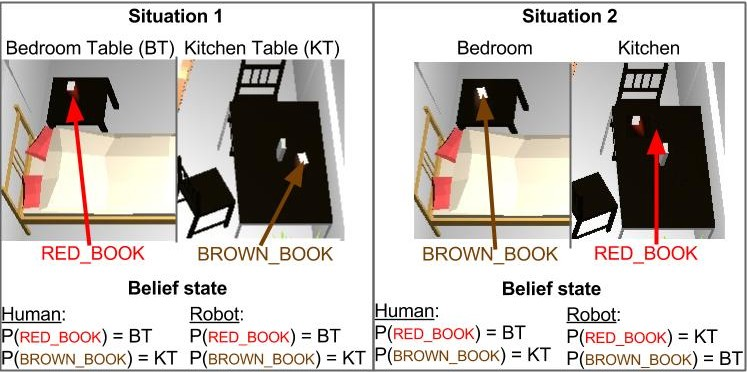
\includegraphics[width=0.89\linewidth]{./img/dbexemple.jpg}
  \caption {Exemple où l'homme a une croyance divergente concernant l'emplacement de deux livres ayant étés inter-changés.}
  \label{fig:dbexemple}
\end{figure}


Nous illustrons la prise en compte de la croyance divergente dans cet exemple avec la figure \ref{fig:overview-mardhis}. Les modifications apportées au modèle initial sont illustrées par les éléments en
orange.

Soit la situation suivante :
l’utilisateur vient de prononcer la phrase « donne moi le livre qui est sur ma table de
chevet ». Comme le montre la figure \ref{fig:overview-mardhis}, logiquement la partition de plus grande probabilité devient celle qui modélise le but utilisateur qui consiste à vouloir lui « apporter
un livre situé sur la table de chevet ». Du point de vue du robot (ROBOT FACTS sur
la figure) ce livre est identifié de façon unique comme étant l’objet RED\_BOOK. Cependant,
du point de vue de l’utilisateur (USER FACTS sur la figure), il est également identifié
de façon unique comme étant l’objet BROWN\_BOOK. Cette situation est considérée
comme divergente et le d-status est réglé sur unique parce qu’il n’y a qu’un seul objet possible qui correspond à cette description dans le modèle de l’utilisateur et que ce dernier est différent de celui également identifié dans la base de faits  du robot. Dans nos travaux, le d-status ne peut prendre que les deux valeurs unique et
other, nous considérons cependant cet élément comme étant catégoriel et non binaire
car nous comptons étendre à terme le nombre des valeurs ainsi considérées (identification de différentes situations comme par exemple le fait que plusieurs objets candidats
présentent une position divergente).
En ce qui concerne la nouvelle action résumée \textit{InformDivergentBelief} introduite pour
résoudre la situation de divergence, les actes de dialogue qui lui sont associés sont déterminés par l’intermédiaire d’heuristiques expertes. Dans cette
première version, lorsqu’un cas de divergence est détecté, idéalement l’action prise par le système doit permettre d’informer l’utilisateur de manière explicite de la présence et de la nature de cette divergence.
Pour ce faire, un acte de dialogue est employé pour informer l’utilisateur sur l’existence d’une divergence quant à la valeur de la position de l’objet "sujet"
de la commande. Grâce à l’émission de cet acte de dialogue l’utilisateur va pouvoir
mettre à jour ses croyances avant de poursuivre son objectif initial. Ainsi, lorsque le
système informera l’utilisateur oralement de la véritable position de l’objet en question, le modèle de croyance utilisateur sera mis à jour en fonction. Ce processus est également illustré dans la figure \ref{fig:overview-mardhis} lorsque l’action \textit{InformDivergentBelief} est sélectionnée
en tant que prochaine action du système (action maître). L’action finalement exécutée
dans l’espace maître sera : \textit{deny(object.location=bedside\_table, object.location=kitchen\_table,
object.type=book, object.color=brown)}, qui sera transformée par le module de Génération de Language Naturel \textit{NLG} dans l’énoncé système suivant "le livre marron n’est plus sur la table de chevet mais sur la table de la cuisine".
% Pour ce qui est de la politique d’interaction, nous envisageons là encore de réaliser
% un apprentissage RL en ligne de la politique. Cependant contrairement aux expériences
% réalisées dans le chapitre 4, nous considérons ici le recours à des interactions faisant
% intervenir de vrais utilisateurs (que ce soit pour l’apprentissage et les tests). Nous décrivons plus précisément les conditions expérimentales dans la section suivante.

\clearpage

\begin{sidewaysfigure}[t!]
%   \vspace{-10pt}
 \centering
 \begin{tabular}{c}
  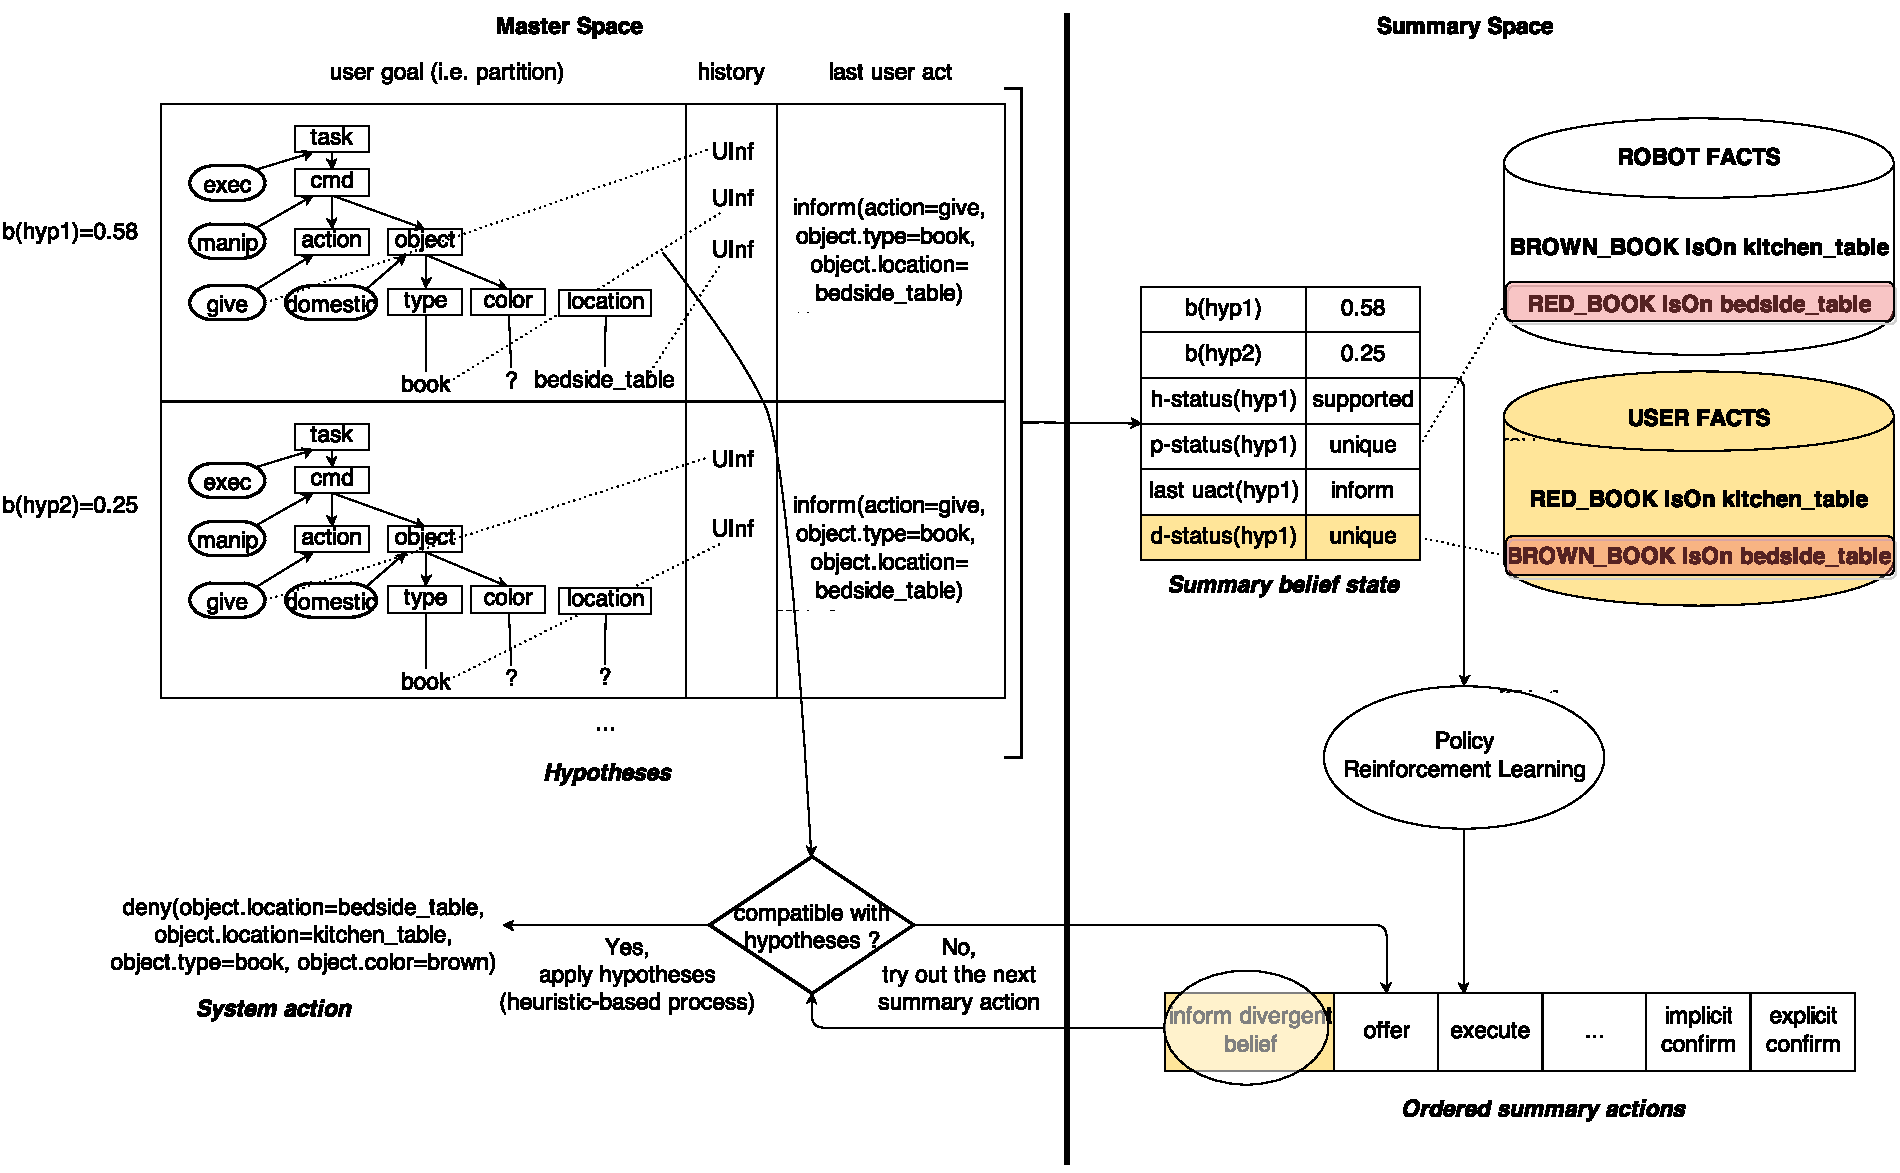
\includegraphics[width=1.0\textwidth]{img/MaRDHIS.pdf}
 \end{tabular}
 \caption{Aperçu de l'extension apportée au système HIS pour prendre en compte les croyances divergentes réalisée par Emmanuel Ferreira dans le cadre du projet MaRDi \cite{ferreira2015phd}.}
 \label{fig:overview-mardhis}
 %  \vspace{-10pt}
\end{sidewaysfigure}


\clearpage


% \subsection{Prise en Compte de l'État Mental}
% As mentioned earlier, an important aspect of the approach is to base our user belief state management on the POMDP framework~\cite{Kaelbling98}. It is a generalisation of the fully-observable Markov Decision Process (MDP), that was first employed to determine an optimal mapping between situations (dialogue states) and actions for the dialogue management problem in~\cite{Levin97}. We try hereafter to recall some of the principles of this approach pertaining to the modifications that will be introduced. More comprehensive descriptions should be sought in the cited papers.
% This framework maintains a probability distribution over dialogue states, called belief states, assuming the true one is unobservable. By doing so, it explicitly handles parts of the inherent uncertainty on the information conveyed inside the Dialogue Manager (DM) (e.g. error prone speech recognition and understanding processes).
% Thus, POMDP can be cast as a continuous space MDP. The latter is a tuple $<B,A,T,R, \gamma>$ 
% , where $B$ is the  belief state space (continuous), $A$ is the discrete action space, $T$ is a set of Markovian transition probabilities, $R$ is the immediate
% reward function, $R: B \times A \times B \rightarrow \Re $ and
% $\gamma \in [0,1]$ the discount factor (discounting long term
% rewards).
% The environment evolves at each time step $t$ to a belief state $b_t$ and
% the agent picks an action $a_t$ according to a policy mapping belief states to actions, $\pi: B \rightarrow A$. Then the belief state changes to $b_{t+1}$ according to the Markovian transition
% probability $b_{t+1} \sim T(.|b_t, a_t) $ and, following this, the agent received a reward $r_t =
% R(b_t, a_t, b_{t+1})$ from the environment.
% The overall problem of this continuous MDP is to derive an optimal policy maximising the reward expectation. Typically the averaged discounted sum over a potentially
% infinite horizon is used, $ \sum^{\infty}_{t=0} {\gamma^t r_t} $. Thus, for a given policy and start belief state
% $b$, this quantity is called the value function: $V^{\pi}(b) =
% E[\sum_{t\ge0}\gamma^t r_t| b_0 = b, \pi] \in \Re^B$. $V^{\ast}$ corresponds to the value function of any optimal policy
% $\pi^{\ast}$.
% The Q-function may be defined as an alternative to the value function. It adds a degree of freedom on the first
% selected action, $Q^{\pi}(b,a) = E[\sum_{t\ge0}\gamma^t r_t|b_0 = b, a_0 = a, \pi] \in \Re^{B \times A}$.
% As well as $V^{\ast}$, $Q^{\ast}$ corresponds to the
% action-value function of any optimal policy $\pi^{\ast}$. If it
% is known, an optimal policy can be directly computed by being
% greedy according to $Q^{\ast}$ ,
% $\pi^{\ast}(b) = \arg\max_a Q^{\ast}(b, a) \forall b \in B$.

% However, real-world POMDP problems are often intractable due to their dimensionality (large belief state and action spaces). Among other techniques, the HIS model~\cite{Young10} circumvents this scaling problem for dialogue management by the use of two main principles. First, it factors the dialogue state into three components: the user goal, the dialogue history and the last user act (see Figure~\ref{fig:overview-mardhis}). The possible user goals are then grouped together into \textit{partitions} on the assumption that all goals from the same partition are equally probable. These partitions are built using the dependencies defined in a domain-specific ontology and the information extracted all along the dialogue from both the user and the system communicative acts. In the standard HIS model, each partition is linked to matching database entities based on its static and dynamic properties that corresponds to the current state of the world (e.g. colour of an object vs spatial relations like \textit{isOn}).
% The combination of a partition, the associated dialogue history, which corresponds here to a finite state machine that keeps track of the grounding status for each convoyed piece of information (e.g. informed or grounded by the user), and a possible last user action forms a dialogue state hypothesis. A probability distribution $b(hyp)$ over the most likely hypotheses is maintained during the dialogue and this distribution constitutes the POMDP's belief state.
% Second, HIS maps both the belief space (hypotheses) and the action space into a much reduced summary space where RL algorithms are tractable.
% The summary state space is the compound of two continuous and three discrete values. Continuous values are the probabilities of the two-first hypotheses $b(hyp1)$ and $b(hyp2)$ while the discrete ones, extracted from the top hypothesis, are the type of the last user act (noted \textit{last\ uact}), a partition status (noted \textit{p-status}) database matching status related to the corresponding goal and a history status (noted \textit{h-status}).
% Likewise system dialogue acts are simplified in a dozen of summary actions like \textit{offer}, \textit{execute}, \textit{explicit-confirm} and \textit{request}. Once the summary actions are ordered by their $Q(b,a)$ scores in descending order by the policy, an handcrafted process checks if the best scored action is compatible with the current set of hypotheses (e.g. for the \textit{confirm} summary act this compatibility test consists in checking if there is something to confirm in the top hypothesis). If they are compatible, an heuristic-based method maps this action back to the master space as the next system response. If not, the process is pursued using the next best scored summary action until a possible action is found.

%> MaRDHIS model
% \begin{figure}[t!]
%    \vspace{-10pt}
%  \centering
%  \begin{tabular}{c}
%   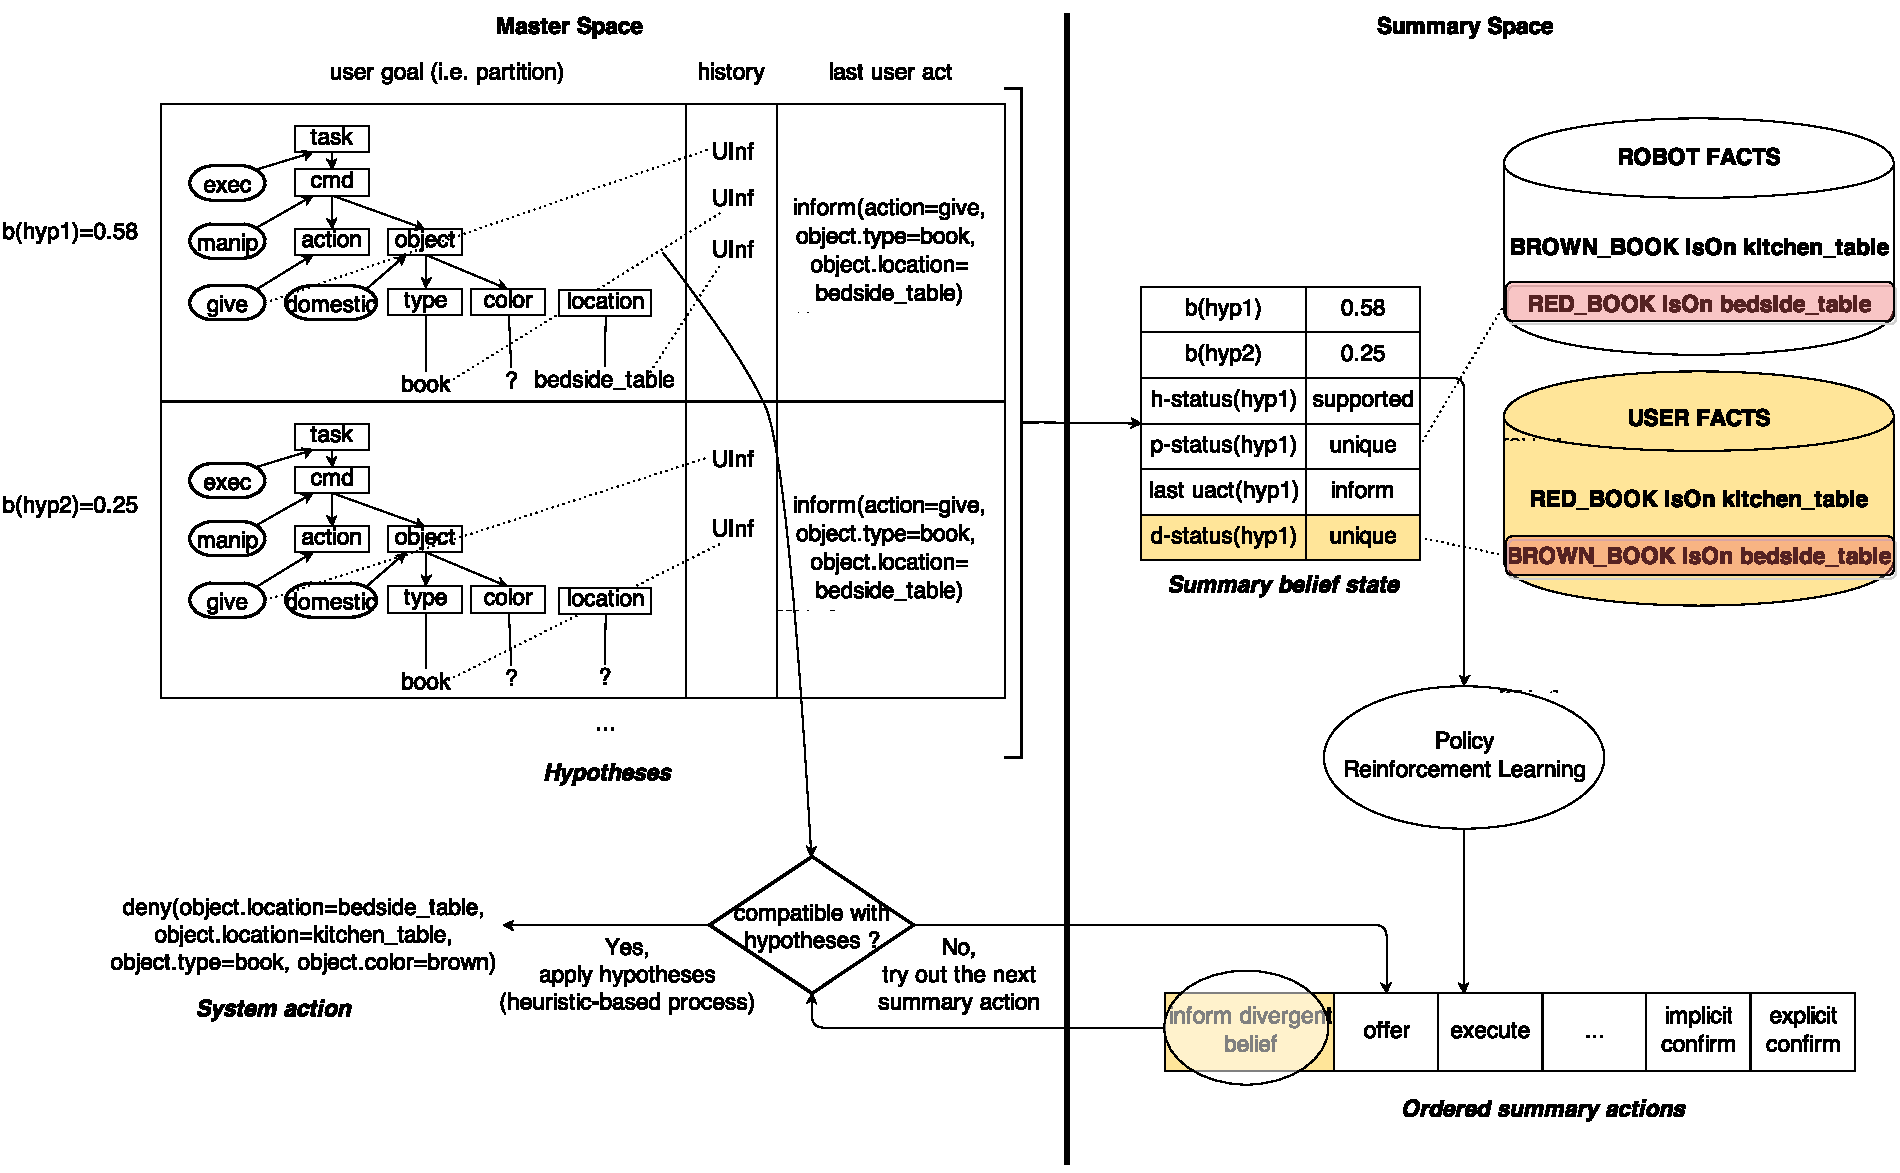
\includegraphics[width=0.98\textwidth]{img/MaRDHIS.pdf}
%  \end{tabular}
%  \caption{Overview of the HIS extension to take into account divergent belief.}
%  \label{fig:overview-mardhis}
%    \vspace{-10pt}
% \end{figure}

% Reviewer 3 => First, I am wondering whether a case when a user has a false belief can be (and needs to be) separately treated with a case with noises in the communicative channel.
% MANU> perso je trouve que le paragrapthe ci-dessous y reponds
%
% Greg> Proposition de simplification:
% GREG> Je trouve que la phrase suivante est "missleading". Notamment le untill she is notified, parceque au final ca peut etre compris comme etant justement une reaction appropriee.
%Indeed, according to her mental belief the user may still want to pursue her goal with an erroneous statement until she is notified, or discovers by herself, that it does not correspond to the true current state of the world. 
% Old
% If the standard HIS framework can properly handle misunderstandings due to noise in the communicative channel, it offers no appropriate mechanism for such a case where the user has a false belief about the state of the world which should impact negatively its communicative acts. Indeed, according to her mental belief the user may still want to pursue her goal with an erroneous statement until she is notified, or discovers by herself, that it does not correspond to the true current state of the world.
% New
% The standard HIS framework can properly handle misunderstandings due to noise in the communicative channel.
% However, misunderstandings can also be introduced in cases where the user has false beliefs, impacting negatively her communicative acts. HIS has no dedicated mechanism to deal with such a situation and so it should react as in front of a %classical uncertainty by keeping requiring the user some confirmations of hypotheses until the request can match the reality, although it could have be resolved since the first turn. 
% classical uncertainty by asking the user to confirm  hypotheses until the request can match the reality, although it could have be resolved since the first turn. 
% Therefore having an appropriate mechanism should improve the quality and efficiency of the dialogue, preventing user to pursue her goal with an erroneous statement.

% So, as illustrated in Figure~\ref{fig:overview-mardhis} and highlighted with the orange items, we propose to extend the summary belief state with an additional status, the
% \textit{divergent belief} status (noted \textit{d-status}), and an additional summary action, \textit{inform divergent belief}.
% % GREG> I think it's hard here to understand what we mean by user facts and how it is different from partition.
% % so I added "(from user's belief model)"
% The \textit{d-status} is employed to trigger the presence of false belief situations by matching the top partition with user facts compiled by the system (see Sec.~\ref{sec:knowledge}) and as such trying to highlight some divergences between the user and the robot points of view. 
% %>>>BEGIN MODIF
% %Reviewer 3 => Are the user facts in Figure 2 maintained as an internal state of the system?  If yes, how is it updated or detected?
% %NEW>
% %****
% Both the user and the robot facts (from the belief models, not to be mistaken with the belief state related to the dialogue representation) are considered as part of the dynamic knowledge resource and are maintained independently of the internal state of the system with the techniques described in Sec.~\ref{sec:knowledge}.
% %>>>END MODIF
% Here we can observe in Figure~\ref{fig:overview-mardhis} that the top partition is about a book located on the bedside table. In the robot model of the world (i.e. robot facts) this book is identified as a unique entity, RED\_BOOK, and \textit{p-status} is set to \textit{unique} accordingly. However, in the user model it is identified as BROWN\_BOOK. This situation can be considered as divergent and \textit{p-status} is set to \textit{unique} too because there is one possible object that corresponds to that description in the user model. 
% %>>>BEGIN MODIF
% %WHY>
% %***
% %Reviewer 3 => The d-status is also unclear although it should be clearly defined. What values it has other than "unique"?  
% %NEW>
% %***
% In this preliminary study \textit{d-status} can only be \textit{unique} or \textit{non-unique}. Further studies may consider more complex cases.
% %>>>END MODIF
% %
% The new summary action is employed for appropriate resolution and removal of the divergence.
% The (real) communicative acts associated to this (generic) action relies on expert design. In this first version, if this action is compatible with the current hypotheses and thus picked up by the system, it explicitly informs the user of the presence and the nature of the divergence. To do so, the system uses a \textit{deny} dialogue act to inform the user about the existence of a divergent point of view and let the user agree on the updated information. 
% % GREG> Maybe explain here that we don't manage the situation when robot is wrong
% % review: It would be good to discuss other issues related to false beliefs
% Consequently, the user may pursue its original goal with the correct property instead of the obsolete one. This process is also illustrated in Figure~\ref{fig:overview-mardhis} when the \textit{inform divergent belief} action is mapped back to the master space.

%%%%%%%%%%%%%%%%%%%%%%%%%%%%%%%%%%%%%%%%%%%%%%%%%%%%%%%%%%%%%%%%%%q


\subsection{Restitution multimodale}
%TODO: rewrite
% Mb do as inputs with a list of modules and some details...
Le robot utilise quatre modules pour gérer la sortie du système afin de transmettre à l'homme la commande choisie par le gestionnaire de dialogue.

\begin{itemize}
\item \textbf{Le module de fission}: il a en charge
le processus de traduction des décisions abstraites (actes de dialogue haut niveau) du système vers des actions verbales et non-verbales (déplacement, prise de position).
Pour l’instant, ce module est basé sur la définition d’un ensemble de règles prenant
en compte la nature de la décision du système (flux 13) et le contexte courant (14).
%TODO corriger le graphique. 
La solution retenue considère également les flux de sorties comme
parallèles (pas de synchronisation fine entre gestes et paroles).

\item \textbf{Le module \textit{NLG}}: ce module est responsable de la génération de langage naturel. Il s'appuie sur des patrons lexicaux pour générer un texte qui soit compréhensible de l'homme afin de le transmettre au \textit{TTS} (18).

\item \textbf{Le module \textit{TTS}}: ce module est responsable de la traduction de texte en parole (Text To Speech), c'est à dire qu'il doit générer un signal sonore correspondant au texte reçu du \textit{NLG} afin qu'il soit émis par les haut-parleurs du robot (19). 
Ce module a été spécialement implémenté par
notre partenaire ACAPELA Group dans le cadre du projet MaRDi. Son originalité réside
dans le fait qu’il repose sur des mécanismes d’interpolations de modèles pour élargir la
richesse expressive de la voix employée tout en offrant un contrôle continu pour moduler
dynamiquement la voix au cours de la synthèse d’un même énoncé \cite{astrinaki2012}. Dans sa version actuelle nous pouvons donc jouer sur trois paramètres simultanément,
à savoir le style de voix (portée, chuchotée ou normale), l’émotion transmise
(ton joyeux, triste ou normal) et la vitesse d’élocution (rapide, lente, normale).
Selon la nature de l’acte de dialogue sélectionné par le système et le contexte interactif,
le module de fission va donc attribuer une étiquette sur l’acte vocal pour que le
module \textit{TTS} puisse faire une synthèse expressive de la phrase générée par le \textit{NLG}. Par
exemple, si l’utilisateur et le robot ne sont pas dans la même pièce le module de fission
va obtenir cette information du contexte (14) et va attribuer l’étiquette indiquant qu’il va falloir que le robot parle plus fort (avec
une voix portée), ou encore si le système informe l’utilisateur qu’il ne peut pas réaliser
l’action (par exemple si l’objet est hors de porté pour lui) alors il pourra faire jouer une
synthèse vocale employant une voix triste.


\item \textbf{Le module \textit{CGG}}: ce module est responsable de la génération des gestes communicatifs (Communicative Gestures Generation). Cela permet d'ajouter de l'expressivité aux réponses du robot en ajoutant une séquence de gestes expressifs pendant que le robot parle. Un ensemble de mouvements correspondants à un panel d'expression a été généré hors ligne. La fission choisit s'il est pertinent d'ajouter un geste expressif à la parole en fonction du contexte (visibilité du robot par l'homme, nécessité d'une gestuelle pour améliorer l'expressivité de la parole) et envoi le cas échéant l'expression à jouer (15). Le CGG se contente d'envoyer de façon séquentielle les différents mouvements correspondant à l'expressivité gestuelle souhaitée.
Suite à un manque de temps ce module n'a pas pu être intégré à l'architecture.
%TODO compléter ceci avec le BML de Javier?
\end{itemize}

% En ce qui concerne la gestuelle et les actions physiques du robot, elles vont se
% faire grâce à l’utilisation d’une interface abstraite, NVBP/MC pour Non-Verbal Behaviour
% Planner and Motor Control en anglais. De par son haut niveau d’abstraction, cette
% dernière nous permet de faire tourner le système de façon similaire que ce soit sur la véritable
% plateforme robotique ou sur l’outil de simulation 3D décrit dans la section 6.3.2.
% Dans notre scénario, deux situations distinctes vont impliquer des mouvements de la
% part du robot. La première est liée à l’exécution de la commande de déplacement d’objet
% utilisateur, cette dernière intervient toujours en fin d’interaction car l’exécution d’une
% commande erronée est également synonyme d’échec dans notre scénario. La seconde
% situation consiste en l’exploration de l’environnement. Elle est utilisée pour acquérir
% des faits symboliques sur des zones non explorées (par exemple aller voir ce qu’il y a
% sur la table de la cuisine).
% Le module de fission utilise l’interface abstraite pour transmettre les commandes
% haut niveau, par exemple move(BLACK\_TAPE, kitchen\_table,bedroom\_bedsidetable) ou explore(
% kitchen\_table). Dans le cas où la plateforme robotique est employée, ces buts vont
% être transmis à un superviseur qui va dans un premier temps planifier les actions devant
% être exécutées par l’intermédiaire d’HATP (pour Human Aware Task Planner) (Alami
% et al., 2006), puis procéder à leur exécution d’après le plan ainsi établi. En simulation,
% l’exécution de ces commandes haut niveau est grandement simplifiée. En effet, elles
% sont traduites en séquence d’actions élémentaires selon des patrons prédéfinis dont nous donnerons quelques exemples dans la section 6.3.2.




\section{Implémentation dans un simulateur robotique}

\subsection{Motivation}
Les systèmes de simulation sont très utilisés en robotique. Ils permettent aux roboticiens d'évaluer et valider leur travaux au niveau d'abstraction souhaité. De cette manière, les projets reposant sur des calculs de haut niveau (interaction, dialogue, supervision) peuvent utiliser un simulateur pour abstraire les niveaux inférieurs (navigation, traitement d'image, manipulation) et éviter que les problèmes qui leur sont liés interfèrent durant l'interaction.

Pour le projet MaRDi, le simulateur est également utile pour partager un même environnement et une même configuration expérimentale entre les différents partenaires. De plus, le système de dialogue reposant sur un gestionnaire de dialogue ayant une politique apprise par renforcement, l'usage de la simulation permet d'effectuer cet apprentissage avec des moyens très réduits \cite{simpar_2014}.

Il est cependant nécessaire que le simulateur soit adapté à l'interaction homme-robot. 
En terme de simulation, deux solutions sont possibles pour ajouter l'homme à la boucle: 1) en modélisant et implémentant leurs comportements et actions, et 2) en utilisant la téléopération pour contrôler les avatars humains.

La première solution présente l'avantage de l'automatisation et ne demande aucune manipulation manuelle. Cette solution est donc moins coûteuse en temps et plus facile à mettre en place. Cependant, selon les caractéristiques humaines requises, il est potentiellement extrêmement complexe d'avoir un modèle de comportement humain réaliste. Les humains sont des entités complexes avec des réactions et comportements quasi impossible à synthétiser de manière satisfaisante. Cette solution est en général retenue pour les études qui n'impliquent pas les comportements humains les plus complexes, comme la navigation ou la manipulation.

Dans la seconde solution, un homme télé-opère un avatar virtuel. La simulation est donc plus complexe à établir car elle nécessite de monopoliser un humain. Cependant, l'avatar du simulateur aura un comportement beaucoup plus réaliste. Pour ce faire, l'environnement doit avoir un rendu visuel réaliste et le contrôle de l'avatar doit être suffisamment intuitif.

D'autres projets de dialogue situé homme-robot reposent sur une étude dans un simulateur. Par exemple pour un scénario de Pick-Place-Carry (Prendre-Placer-Transporter) \cite{Lucignano13}, de robot barman \cite{stiefelhagen07} ou de navigation dans un environnent virtuel \cite{byron06}. Cependant, peu de travaux considèrent l'environnement de simulation comme moyen pour l'acquisition du corpus de dialogue situé ou comme moyen de tester l'apprentissage de politique en ligne.
%Indeed, most of the previous works in situated dialogue for HRI resorted to a preliminary Wizard-of-Oz (WoZ) experiment, where a human remotely operates the robot %, and then, used the collected data to train both a user simulator and an error model to pursue the dialogue policy learning without the use of any new real interactions
%
En effet, la plupart repose sur des expériences en magicien d'Oz \cite{prommer06,stiefelhagen07,rieser08}. 
%However, the WoZ technique is both time consuming and an expensive method.



\subsection{Choix du simulateur}
Dans le domaine de la robotique, de nombreux simulateurs sont disponibles. Nous pouvons citer la suite Player/Stage/Gazebo ~\cite{psg-1232}, la plateforme de simulation intégrée OpenHRP \cite{Nakaoka|iros07}, l'architecture logicielle multiplateforme OpenRAVE \cite{diankov_thesis} ou même le simulateur  commercial V-REP \cite{Freese2010}. Cependant, seuls quelques-uns d'entre eux sont adaptés à l'interaction homme-robot. Ils limitent généralement les comportements des agents humains à des mouvements et des capacités d'interaction relativement simple, ce qui constitue  l'une des raisons pour laquelle les simulations de HRI ont été menées jusqu'à présent dans des configuration de \emph{télé-opération}, où seul le robot et l'environnement (et pas l'agent humain) sont en fait simulés. Les simulateurs robotiques USARSim \cite{Lewis07usarsim} et MORSE \cite{morse_simpar_2012, simparmorse2014} sont tous deux utilisés dans des dizaines d'études HRI en raison de leur capacité à contrôler un agent humain. Cependant, MORSE présente plusieurs avantages spécifiques qui ont motivé notre choix.

% Open-source / COMMUNAUTEE / supports actifs middleware
MORSE est un simulateur open-source, avec une communauté très active, qui a été développé spécifiquement pour la simulation robotique. Il prend en charge une large gamme de middleware (par exemple ROS, YARP, pocolibs) ainsi que des implémentations fiables et réalistes des capteurs et des actionneurs qui facilitent l'intégration sur de véritables plateformes robotiques.
% Capteurs / actionneurs avec le niveau d'abstraction
En outre, MORSE offre une configuration de simulation adaptable en permettant à des robots virtuels d'interagir avec l'environnement virtuel en utilisant soit des capteurs/actionneurs réalistes ou des capteurs/actionneurs ayant un niveau d'abstraction supérieur. De ce fait, les roboticiens peuvent contrôler le coût de calcul de traitement des données de bas niveau en exploitant les sorties de haut niveau à partir de composants "irréalistes".
%
Par exemple, Morse fournit à la fois une caméra de vision et
un capteur dit "caméra sémantique". Alors que la première caméra fournit une image brute (pixels) en tant que sortie, la seconde
donne directement les noms des objets perçus et leurs positions dans la scène.
Ce dernier capteur évite pour les utilisateurs à devoir effectuer la reconnaissance et les processus de localisation d'objets lors de la focalisation sur les problématiques de niveau supérieur.

% Rendu réaliste
De plus, MORSE repose sur "Blender Game Engine",
un moteur d'exécution 3D en temps réel intégré au toolkit de modélisation open-source Blender, à la fois pour la 3D avancé (OpenGL Shader) et
pour la simulation de la physique (basée sur le moteur physique BULLET).
Cette configuration permet un rendu réaliste d'environnement complexe et fournit une interface utilisateur graphique immersive, qui est une caractéristique nécessaire %pour le contrôle immersif d'un avatar humain.
pour la modélisation HRI.

% des commandes avatar humaines
Dans MORSE, l'avatar humain peut être contrôlé par un opérateur humain ou directement par le biais de scripts externes comme tout autre robot.


% In the robotic field, many simulators are available. We can name the Player/Stage/Gazebo suite~\cite{psg-1232}, the integrated simulation platform OpenHRP \cite{nakaoka|iros07}, the cross-platform software architecture OpenRAVE \cite{diankov_thesis} or even the commercial simulator V-REP \cite{Freese2010}. However, only a few of them are very well suited to HRI. They generally limit human agent behaviours to relatively simple motions and interaction capacities which is one of the reasons why HRI simulations so far have been carried out in \emph{tele-operation} settings, where only the robot and the environment, but not the human agent, are actually simulated. Robotic simulators USARSim \cite{Lewis07usarsim} and MORSE \cite{morse_simpar_2012,simparmorse2014} are both used in dozens of HRI studies due to their explicit support for controlling a human agent. However, the latter has several specific advantages that motivated our choice. 

% % open-source / active communauty / middleware supports 
% MORSE is an open-source simulator, with a very active community, that was developed specifically for robotic simulation. It supports a wide range of middleware (e.g. ROS, YARP, pocolibs) as well as reliable implementations of realistic sensors and actuators which ease the integration on real robotic platforms afterwards.
% % Sensors / actuators with different level of abstraction
% Moreover, MORSE offers an adaptable simulation setup by allowing virtual robots to interact with the virtual environment through both realistic sensors/actuators and higher level ones. Thereby, roboticists can control the related computation cost of low level data processing by exploiting high level outputs from unrealistic components. 
% %
% For example, MORSE provides both a vision camera and a
% semantic camera sensor. While the first camera provides a rough image (i.e. raw pixels) as output, the second one
% gives directly the names of the perceived objects and their positions in the scene. 
% The latter sensor avoids practitioners to perform object recognition and localization processes when focusing on higher level issues.

% % Realistic rendering
% Furthermore, MORSE relies on the Blender Game Engine,
% a real-time 3D runtime integrated to the open-source Blender
% modelling toolkit, for both advanced 3D (OpenGL shader) and
% physics simulation (based on the BULLET physics engine).
% This setup allows realistic rendering of complex environment and provides an immersive graphical user interface, which is a required feature %for immersive control of a human avatar.
% for HRI modelling. 

% % Human avatar controls
% In MORSE, the human avatar can be controlled by a human operator or directly through external scripts as any other robot.  

\begin{figure}[ht!]
 \centering
 \begin{tabular}{cc}
  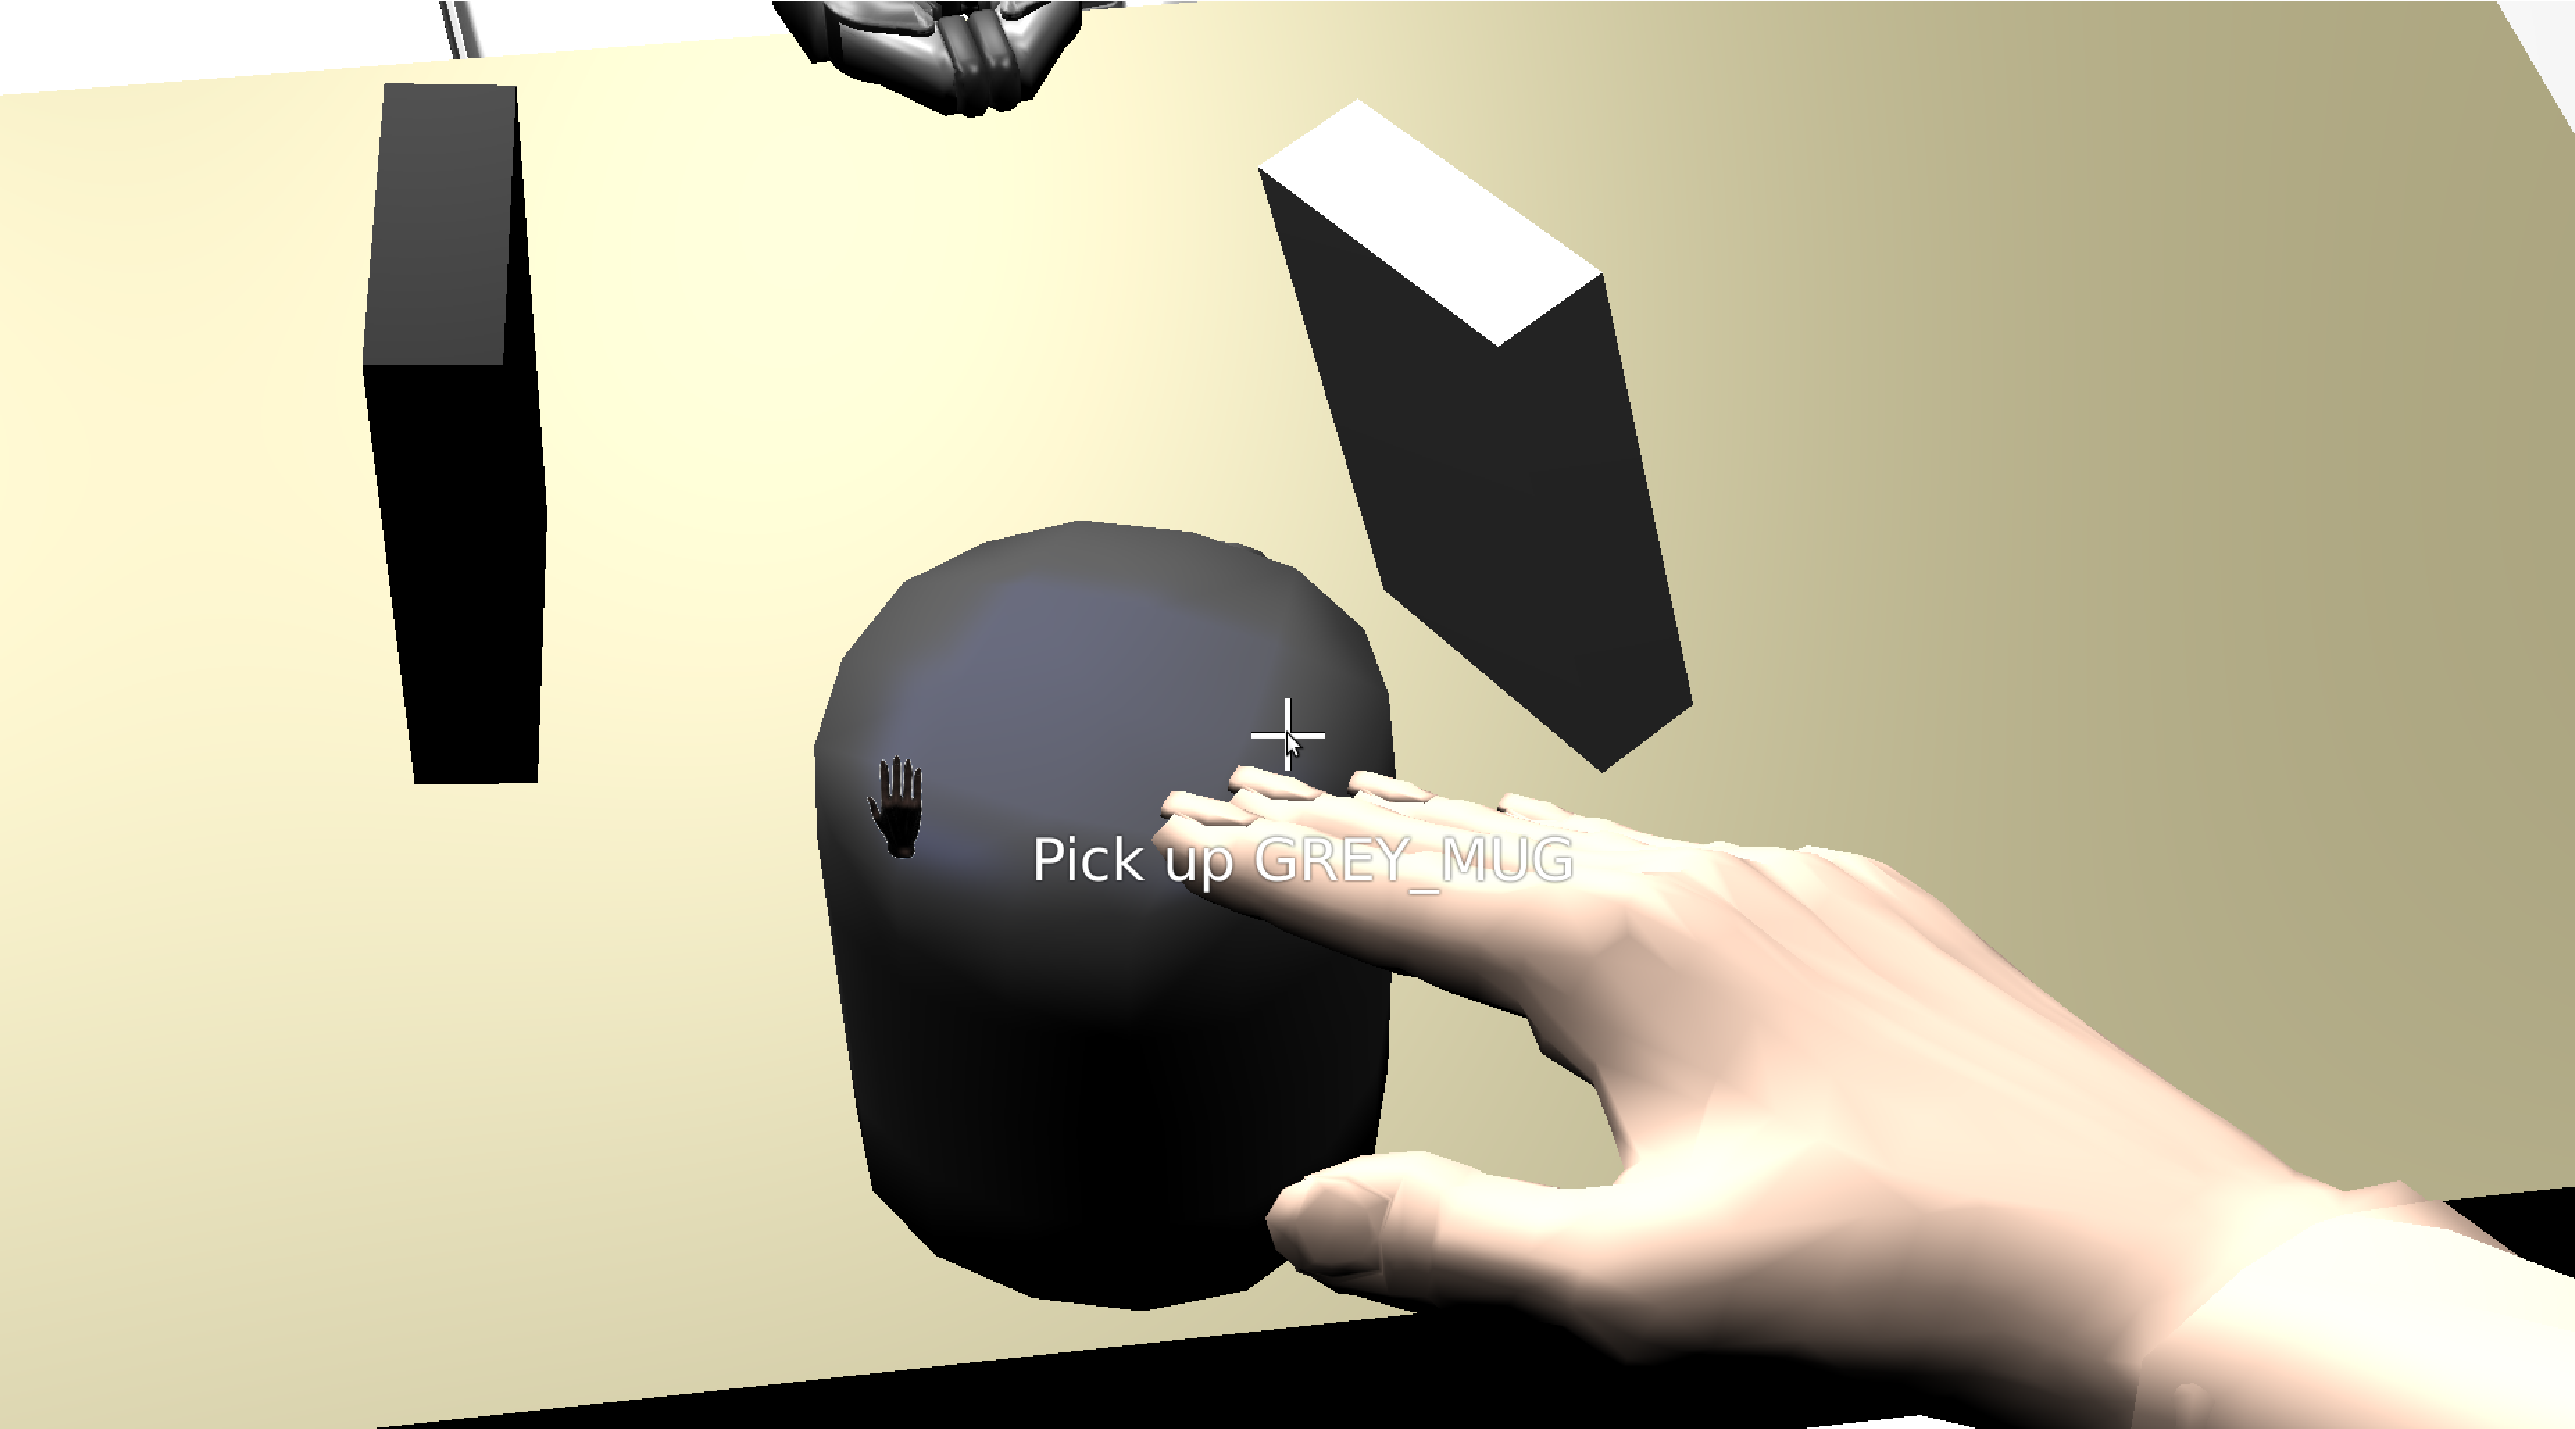
\includegraphics[width=0.475\textwidth]{img/Screenshot_from_2014-04-29_14_02_14.png} &
  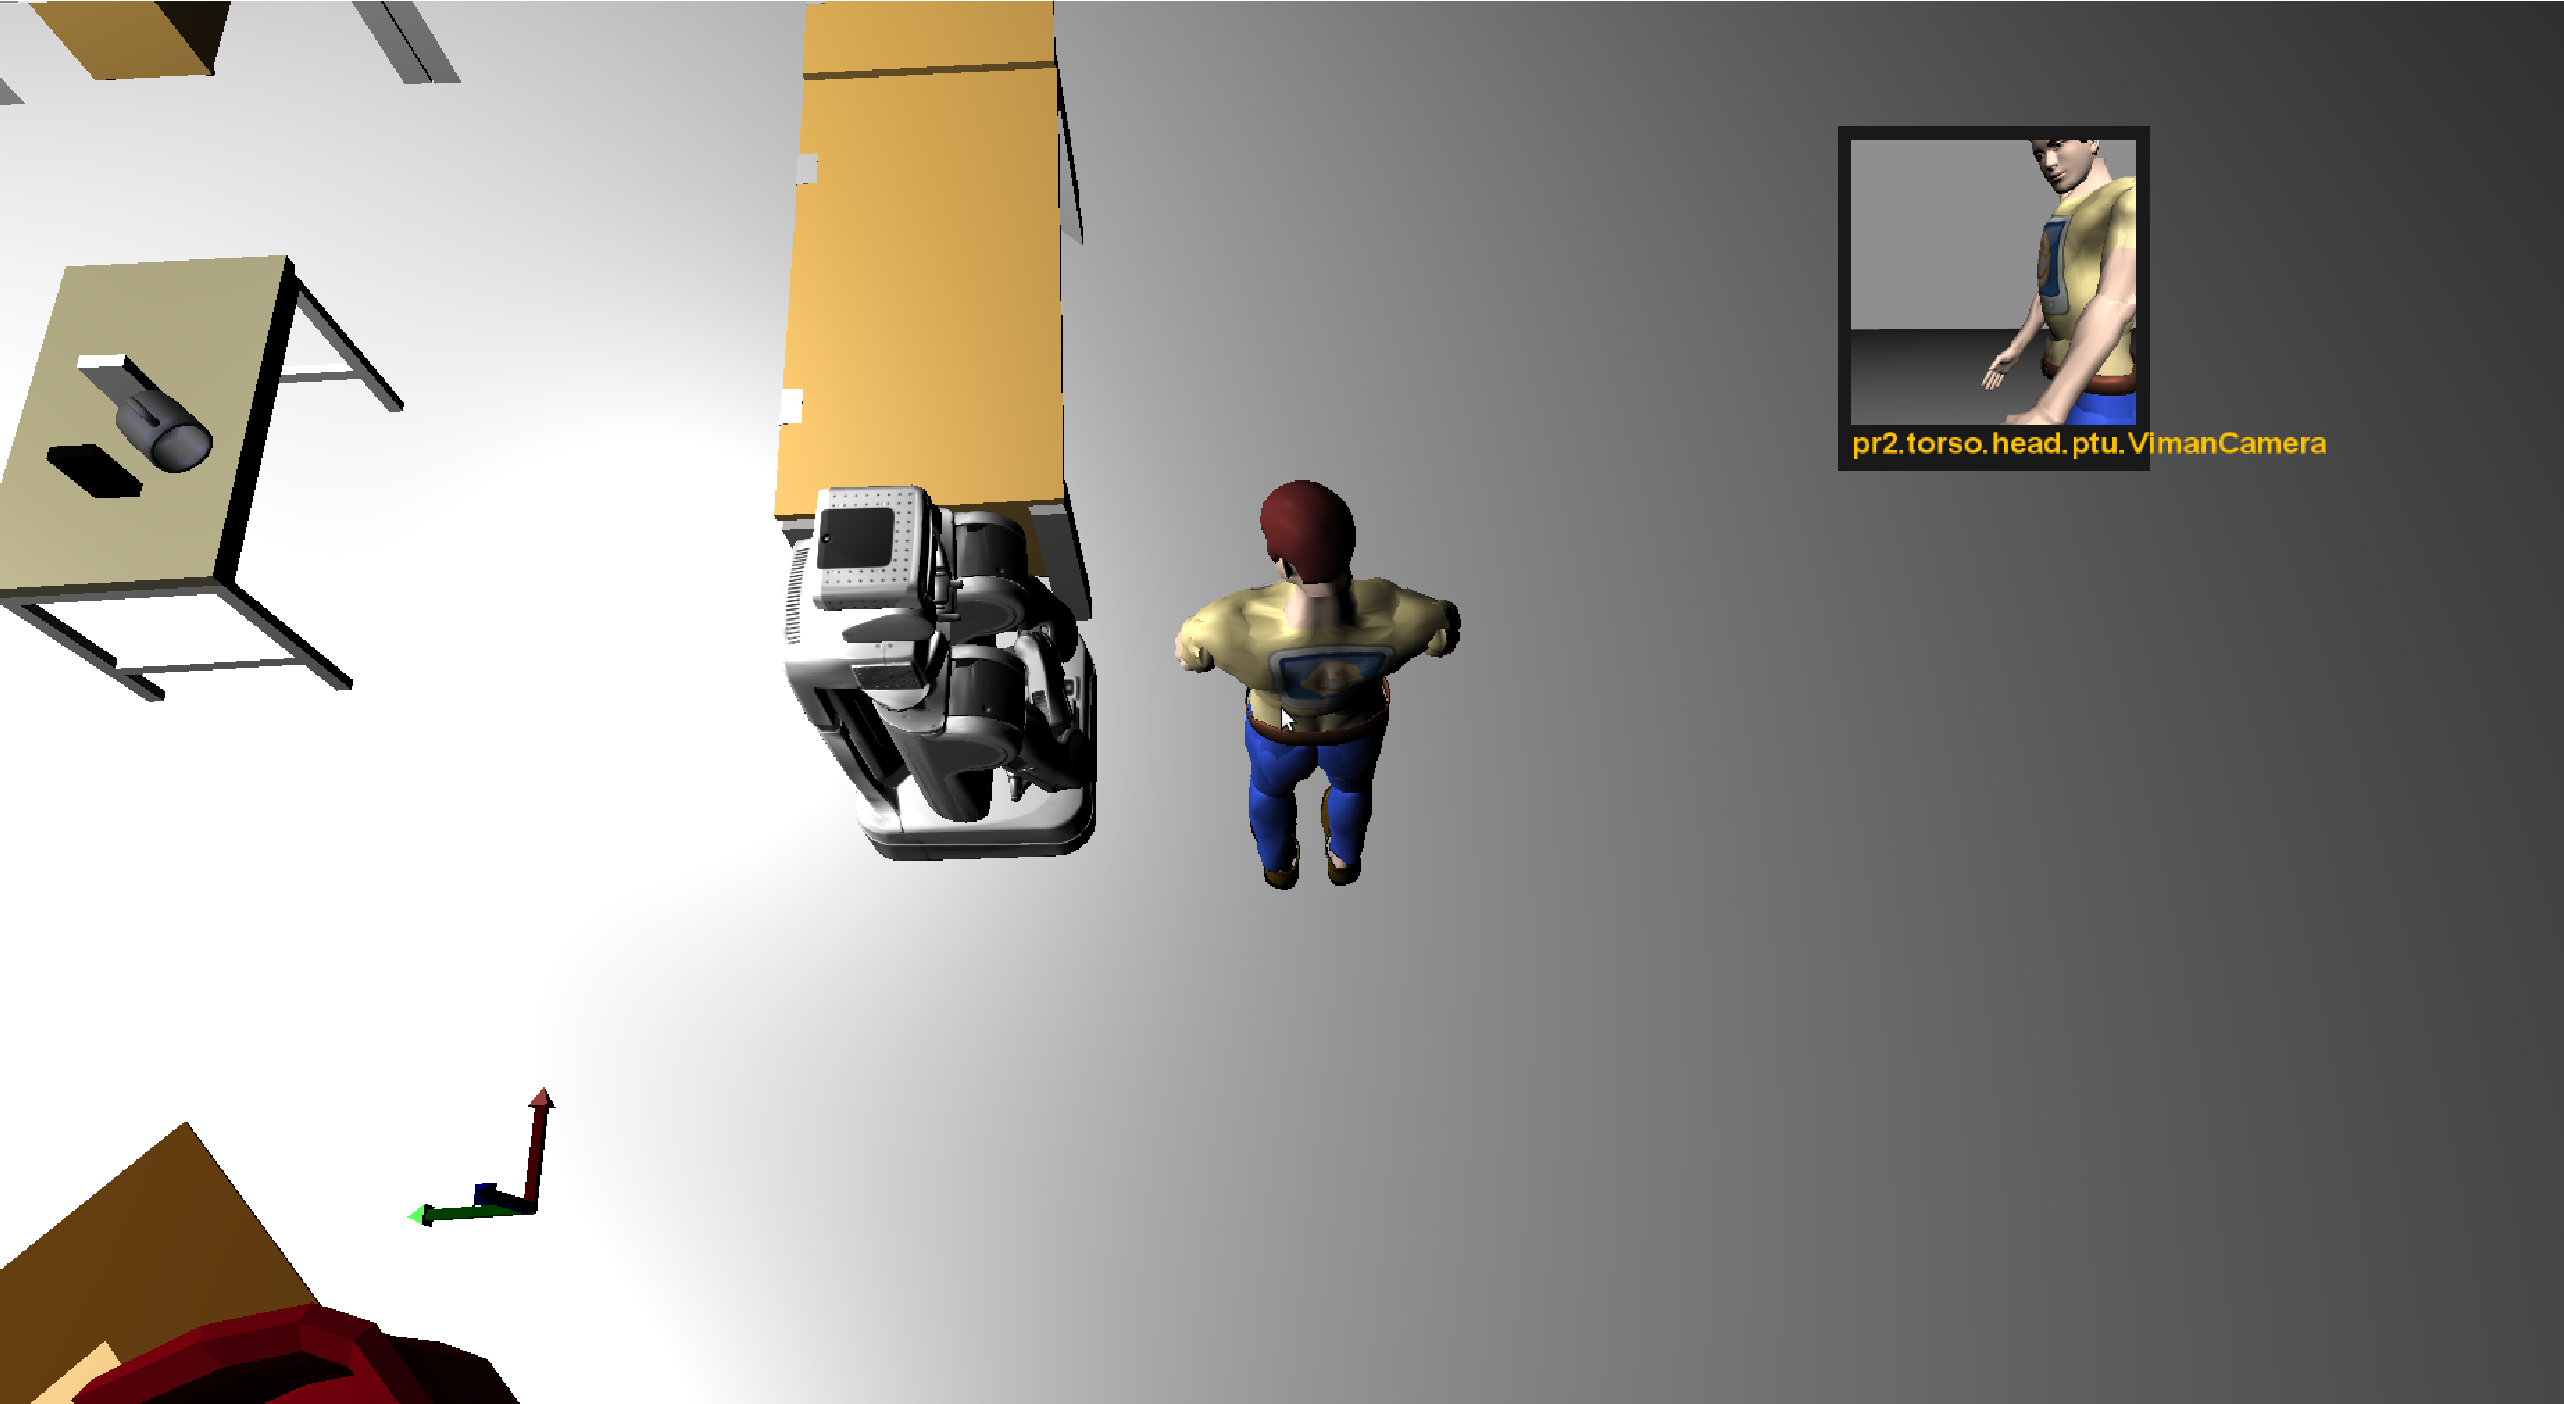
\includegraphics[width=0.475\textwidth]{img/Screenshot_from_2014-04-29_14_21_24.png}
 \end{tabular}
 \caption{Avatar humain attrapant un objet, contrôlé par un opérateur (image de gauche) et l'avatar humain en vue à la troisième personne (image de droite).}
 \label{fig:human_morse}
 %  \vspace{-3pt}
 \end{figure}

Dans le premier cas, l'opérateur contrôle l'humain virtuel de manière immersive (voir la figure \ref{fig:human_morse}) en termes de déplacement, de regard, et des interactions sur l'environnement, tel que la manipulation d'objets (par exemple, saisir ou déposer un objet).

Dans le second cas, l'avatar est contrôlé par programme en utilisant des actionneurs MORSE standard. A titre d'exemple, il est possible d'utiliser un actionneur "waypoint" (point de cheminement) sur l'humain pour définir un trajet qu'il doit suivre.


%%%%%%%%%%%%%%%%%%%%%%%%%%%%%%%%%%%%%%%%%%%%%%%%%%%
\subsection{Simulation de l'interaction}

%Explain why it is interesting for us to simulate + mainly phase 1
La simulation de l'interaction nous permet dans notre cas d'obtenir rapidement un moyen d'entraîner le système de dialogue et de tester la validité de notre architecture pour la phase de détermination de but décrite en \ref{sec:phase1}.
Les phases d'élaboration de but et d'exécution seront donc simplifiées au maximum.

Dans notre scénario, une personne handicapée est dans son appartement de trois pièces et possède un robot pour l'assister dans les tâches quotidiennes.
Le but ici est de faire en sorte que le système robotique puisse comprendre, en raisonnant sur les paroles de l'homme, les gestes et l'environnement, la requête de l'homme concernant les objets. Les objets sont limités ici aux objets qui peuvent être saisis comme des livres, des DVDs et des tasses, qui ont divers couleurs, type, position et un identifiant unique.

Nous utilisons le robot Pr2 dans le simulateur car c'est la plateforme que nous utilisons au LAAS-CNRS. Le Pr2 est déjà présent dans les modèles de MORSE, le rendant directement utilisable. Nous avons ajouté une caméra symbolique (MORSE semantic camera) au modèle standard afin qu'il puisse réaliser la reconnaissance d'objet. Nous avons également ajouté un actionneur appelé "teleport" pour bouger le robot à une position donnée en évitant ainsi d'avoir à gérer la navigation et en gagnant le temps du déplacement. Nous utilisons un modèle virtuel de l'environnement physique dans lequel le robot réel sera testé. Enfin, nous ajoutons un avatar humain. La configuration expérimentale est schématisée à la figure \ref{fig:simusetup}. L'humain utilise le clavier (1) pour contrôler son avatar et a un retour visuel sur l'écran (2). Un casque audio avec micro intégré est utilisé pour dialoguer avec le système (3 et 4). Les flux 5 et 6 seront détaillés en section \ref{section:actions}. 
% TODO take a screenshot of env with objects

\begin{figure}[ht!]
 \centering
  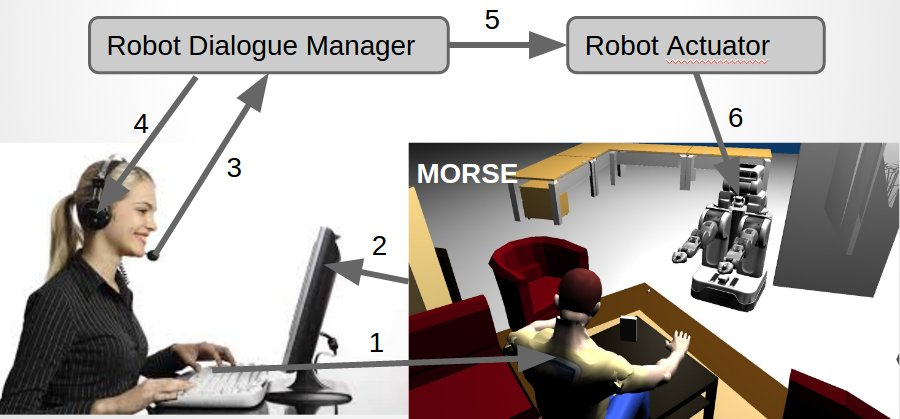
\includegraphics[width=0.89\linewidth]{./img/simusetup.jpg}
  \caption {Configuration expérimentale pour la simulation dans morse avec un agent humain contrôlant l'avatar du simulateur.}
  \label{fig:simusetup}
\end{figure}

 
Au début de la simulation, un script positionne des objets au hasard dans des zones prédéfinies (comme la table de la cuisine, celle du salon, l'étagère de la chambre...). Ces zones sont appelées des zones de manipulation. Cela nous permet d'utiliser différentes configurations d'environnement sans changer le fichier d'initialisation (MORSE builder script).

%-----------------------------------------------%
\subsection{Simulation de l'exécution}
\label{section:actions}
%TODO
%-> Why we need these actions?
%   -> Simulation more interactive and realistic
%    -> Objective fulfillment evaluation according to robot action (users satisfaction)
Pour permettre aux utilisateurs d'évaluer l'accomplissement de sa requête (par exemple, est-ce que le robot rapporte le bon objet), nous avons développé une librairie abstraite d'actions haut niveau réalisable par le robot. Ces actions haut niveaux seront combinées pour accomplir l'objectif énoncé par l'utilisateur. Leur haut niveau d'abstraction permet ici de pouvoir accomplir le but utilisateur sans avoir recours au planificateur ou à la supervision et donc de contourner les phases deux et trois décrites en section \ref{sec:phase2} et \ref{sec:phase3}.

La liste des actions abstraites est la suivante:

\begin{itemize}

% Move robot to manipulation area
\item \textit{Move}: pour explorer l'environnement ou rapporter un objet, le robot a besoin de se déplacer vers les zones de manipulation. Pour ce faire, nous utilisons l'actionneur \textit{teleport} de MORSE. Cet actionneur permet de déplacer instantanément le robot à l'endroit désiré. Nous avons défini une fonction de script pour bouger le robot vers chaque zone de manipulation définie. De cette façon, le robot peut se rendre à chaque position pour prendre un objet ou explorer une zone pour obtenir des informations contextuelles.

% Explore an area
\item \textit{Explore}: le robot est capable de scanner une zone de manipulation. Pour rendre cette action possible, une caméra symbolique a été ajoutée à la tête du robot. La tête se déplace séquentiellement pour scanner l'environnement.

% Grab object
\item \textit{Grab}: le robot peut prendre un objet. Pour réaliser cette action, le service \textit{grasp} lié au Pr2 de MORSE est utilisé. Nous précisons le nom de l'objet qu'il doit attraper et si l'objet est proche de la pince du robot, il sera placé au niveau de celle-ci et lié à son déplacement. De la même façon, nous avons ajouté une fonction \textit{Drop} qui prend comme paramètre la zone dans laquelle l'objet doit être déposé. Le robot relâchera alors l'objet sur le meuble correspondant.

% Give object
\item \textit{Give}: la dernière action est de donner l'objet à l'humain. Pour ce faire, le robot se déplace vers la position de l'homme puis déploie son bras vers l'homme afin de lui remettre l'objet. Nous utilisons simplement l'armature du robot pour contrôler son bras.
\end{itemize}

Ces actions haut niveau permettent d'effectuer des expérimentations avec un système réalisant la détermination de la demande utilisateur jusqu'à la réalisation et l'exécution d'actions, tout en nous focalisant sur la partie dialogue situé (dans l'univers simulé). Cela rend possible d'entraîner le système de dialogue et de faire des premières évaluations de façon bien plus rapide et moins coûteuse en terme de ressources requises.

\subsection{Expérimentation et résultats}
% In this "proof of concept" study we chose to deal with a limited expert panel, composed of 6 subjects (2 females and 4 males of around 25 years old), in order to focus on the capacity of the system to learn from scratch using a limited set of interactions. The advantage is that the collected data sufficiently explore the state and action spaces during the online learning to be exploited in offline learning (using batch samples).

% At the beginning of each dialogue, a specific goal (here a command) is randomly generated taking into account the simulated environment settings and the current interaction history in order to select a possible command. For example, "You want the robot to give you the white book on the kitchen table". No experimenter has any idea of the chosen configuration of the system with which he is interacting. So, we basically compare a hand-crafted expert dialogue policy (noted HDC) to a learned one (noted LEARNED). The latter was trained using a small set of expert users which first performed $60$ dialogues in an online learning setting.

% In the complete multimodal architecture, each interaction takes from $7$ to $10$ minutes to complete (objects detection, robot movements, etc.).  So, without loss of generality, a practical workaround to speed-up the testing process consisted in using a fixed representation of the scene (a screenshot from the human point of view) and a web-based multimodal GUI instead of the full simulation setup.  Overall, $84$ dialogues for both the two proposed systems were recorded with $6$ distinct subjects. At the end of each interaction users evaluated the system in terms of task completion. The learned policy were configured to act greedily according to the value function. Results are those gathered in test condition where exploration is not allowed. All the dialogues were  recorded both in terms of audio and various kinds of meta-information (e.g. ASR N-Best list, dialogue manager detected gestures and related timestamps, etc.) but also high level annotations (e.g. environment settings, pursued goal, task success). As an illustration, a short interaction, translated from French, is given in Table~\ref{table:hri-example}.

% \begin{table}
% \centering
% \small
% \begin{tabular}{|c|c|l|}
%   \hline
%   \multirow{3}{*}{R1} & DA & hello() \\
%     & NLG/TTS & Can I help you ?\\
%     \hline
%   \multirow{3}{*}{U1} & ASR & Can you put the book in my bedroom? \\
%   	& SLU & inform(action=move,desc=in,room=bedroom)\\
%     \hline
%   \multirow{3}{*}{R2} & DA & confreq(type=book,position) \\
%     & NLG/TTS & Sorry but where is the book you are talking about?\\
%     \hline
%   \multirow{3}{*}{U3} & ASR & I am talking about this one \\
%   	& SLU & inform(idobj=?)\\
%     & GRU & pointsAt BLUE\_BOOK 1395848705.31\\
%    \hline
%     \multirow{4}{*}{R3} & & execute(action=move,destination=bedroom\_bedsidetable,\\
%      & DA & idobj=BLUE\_BOOK,position=livingroom\_table,type=book,\\
%     & &color=blue) \\
%     & NVBP/MC & move(BLUE\_BOOK,livingroom\_table,bedroom\_bedsidetable)\\
%     & NLG/TTS & Ok, I will put the blue book on your bedside table\\
%     \hline
% \end{tabular}
%  \caption{Example of a multimodal dialogue.}
%  \label{table:hri-example}
%  \vspace{-20pt}
%  \end{table}
 
% The results obtained are $14.3$ for the HDC method and $17.6$ for the LEARNED one. These results are given in terms of mean discounted cumulative rewards~\cite{Sutton98}. According to the reward function definition, this metric expresses in a single real value the two variables of improvement, namely the success rate (accuracy) and the number of turns until dialogue end (time efficiency). So, here the HDC policy manages the dialogue with $86\%$ of success rate in an average of $4.8$ turns against respectively $93\%$ and $2.9$ turns for the LEARNED one.  The difference observed between the two methods can be mainly explained by a more accurate and less frequent usage of request of confirmation as well as an expected more fined-grained uncertainty management for the LEARNED method. Thus, these results clearly both demonstrates the ability of the overall architecture (simulation software + multimodal dialogue system) to learn an efficient dialogue policy using few dialogue examples and shows the interest of considering RL methods rather than a hand-crafted fixed and suboptimal policy. Indeed, only $60$ training dialogues are enough to outperform the HDC by more than $3$ points.



Une première étude a été menée pour montrer la capacité du système à apprendre la politique du gestionnaire de dialogue. Cette étude a permis de montrer que le système de simulation permet d'entraîner et d'améliorer significativement et avec un coût réduit le système de dialogue. Les détails et résultats de cette expérimentation disponibles dans \cite{simpar_2014} ne seront pas discutés ici afin de nous focaliser sur l'aspect gestion de croyance.

La seconde expérimentation menée sur le simulateur robotique morse concerne l'évaluation de l'amélioration du système de gestion de dialogue situé multimodal lors de la prise en compte des croyances erronées, comme présenté en section \ref{sec:mentalStateDial}.
Nous nous focalisons donc sur des scénarios où une divergence de croyance est présente entre le modèle d'état d'esprit de l'homme et celui du robot. 
Dans une configuration réaliste, ces scénarios nécessitent des interactions d'une certaine durée pour faire apparaître une croyance divergente. Pour contourner ce processus coûteux en temps dans notre configuration d'évaluation, nous proposons directement un but erroné à l'utilisateur au début de l'interaction. 
Par conséquent, une fausse croyance sur la localisation d'un objet non visible de l'homme est automatiquement ajoutée. Même si cette situation est créée de façon artificielle, le même comportement peut être obtenu en utilisant notre système d'évaluation spatiale, comme présenté en section \ref{sec:ResChap2}.

Par conséquent, cette configuration a été utilisée pour évaluer la capacité de notre système à gérer à la fois les tâches de manipulation classique (CLASSIC) et de fausse croyance (FB pour False Belief).
Pour ce faire, nous comparons un système ayant connaissance des croyances de l'homme (BA pour Belief Aware) avec un système n'ayant pas de gestion de croyance (BU pour Belief Unaware). Ces deux systèmes ont des politiques apprises par l'interaction avec deux utilisateurs experts ayant réalisé $60$ dialogues.

Dans la configuration d'évaluation, $10$ dialogues ont été enregistrés pour \textit{BA} et \textit{BU}, ces dialogues provenant de 6 sujets distincts (deux femmes et quatre hommes d'environ 25 ans), soit au total 120 dialogues. $30$\% de ces dialogues impliquaient des tâches de type \textit{FB}. Les sujets n'avaient pas connaissance de la configuration du système, les tests ayant été présentés dans un ordre aléatoire. À la fin de l'interaction, les utilisateurs évaluent le système en terme de réussite de la tâche avec un questionnaire en ligne.

%(p 193 thèse Manu)

%> EXPERIMENTAL SETUP

% The DM implements the extended HIS framework described in Sec.~\ref{sec:dialogue}. For the reinforcement learning setup, the sample-efficient KTD-SARSA RL algorithm~\cite{Daubigney12} in combination with the Bonus Greedy exploration scheme enables online learning of dialogue strategy from scratch, as in~\cite{Ferreira13b}. A reward function is defined to penalise the DM by $-1$ for each dialogue turn and give it a $+20$ if the right command is performed at the end of the interaction, $0$ otherwise. To convey the DM action back to the user, a rule-based fission module is employed that splits the high level DM decision into verbal and non-verbal actions. The robot speech outputs are generated by chaining a template-based Natural Language Generation (NLG) module, which converts the sequence of concepts into text, to a Text-To-Speech (TTS) component based on the commercial Acapela TTS system\footnote{http://www.acapela-group.com/index.html}. A Non-verbal Behaviour Planning and Motor Control (NVBP/MC) module produces robot postures and gestures by translating the non-verbal actions into a sequence of abstract actions such as \textit{grasp}, \textit{moveTo}, \textit{release} which are then executed in the simulated environment.


\begin{table}
 \vspace{-10pt}
\centering
\scriptsize
\renewcommand{\arraystretch}{1.2}
\begin{tabular}{|c||*{3}{c|cc||}*{3}{c|cc|}}


\multicolumn{1}{c}{} & \multicolumn{3}{c}{BU} & \multicolumn{3}{c}{BA} \\

\hline
TASK  & $Avg.R$ & $Length$ & $SuccR$  
      & $Avg.R$ & $Length$ & $SuccR$  \\ 
\hline
 	CLASSIC & 17.62 & 2.95 & 0.93 
            & 17.69 & 2.88 &  0.93 \\
   	FB	& 12.72 & 5.94 &  0.83 
        & 13.89 & 4.78&  0.83	 \\
    \hline
    ALL & 16.15 & 3.85&  0.9 
        & 16.55 & 3.45& 0.9 \\
        
\hline
\end{tabular}
\caption{Performance du système sur des tâches classiques (CLASSIC), de fausse croyance (FB) et globales (ALL) en terme de moyenne sur les récompenses cumulées
 (Avg.R), de longueur moyenne des dialogues en nombre de tours (Length) et de taux de succès moyen (SuccR).}
 \label{table:hri-perfs}    
 \vspace{-10pt}
\end{table}

Le tableau \ref{table:hri-perfs} est rempli avec les performances obtenues par les deux configurations discutées ci-dessus en considérant les tâches CLASSIC et FB. Ces résultats sont d'abord donnés en terme de moyenne sur les récompenses cumulées (Avg.R). D'après la définition de la fonction de récompense, cette métrique exprime dans une seule valeur les deux variables d'amélioration, le taux de succès (précision) et le nombre de tours avant la fin du dialogue (efficacité temporelle). Ces deux métriques sont également représentées. Les résultats dans le tableau \ref{table:hri-perfs} sont une moyenne des $60$ dialogues réalisés pour chaque système.



Sur les tâches CLASSIC la performance entre BU et BA doit être considérée comme similaire. Ainsi, le mécanisme de résolution de croyance divergente ne semble pas influer sur la gestion du dialogue dans les situations sans croyance divergente.  La politique testée est apprise, par conséquent le processus d'attribution d'action est optimisée avec un degré supplémentaire de complexité (plus grand espace état / action que dans BU), donc une perte aurait pu être observée.

Les performances entre BU et BA sur les tâches FB apparaissent en faveur de BA (taux plus élevé de réussite et un petit gain d'efficacité au niveau du temps  du processus de gestion du dialogue: gain moyen d'un tour).
%
%TODO translate?

% However the quantitative comparison between the system configurations is not ensured to be relevant due to the relatively high confidence interval on considered metrics (e.g. success rate confidence interval for row FB is around $0.2$ for all system configurations).
% Two main reasons account for this status quo. First, a limited amount of observations involving the different system configurations (due to experimental cost). Second, the expected marginal gain in terms of the considered metrics. Indeed, the current system is learnt on some overall task completion and efficiency criterion. However solving divergent belief situations in a pick and place scenario can not be considered a critical factor influencing these criterion greatly but just a way to cope with an additional (not dominant) degree of uncertainty and to improve user experience and naturalness of the interaction with the embodied agent. 

\begin{table}
%\vspace{-10pt}
\centering
\scriptsize
  \begin{tabular}{llll}
  \hline
  $R_1$: & Puis-je vous aider? & $U_1$: & Apporte moi le livre qui est sur ma table de nuit.\\
\end{tabular}
  \vfill
  \subfigure[][]{
  \begin{tabular}{p{0.5cm} p{4.0cm}}
  $R_2$: & \textbf{Le livre marron n'est plus sur la table de nuit, il a été déplacé vers la cuisine.}\\
  $U_2$: & D'accord, apporte le moi\\
  $R_3$: & Je vous apporte le livre marron qui est sur la table de la cuisine. \\
  \hline
\end{tabular}
  }%
  \qquad
  \subfigure[][]{
   \begin{tabular}{p{0.5cm} p{4.0cm}}
  $R_2$: & Voulez-vous le rouge?\\
  $U_2$: & Non, le marron. \\
  $R_3$: & Il n'y a pas de livre marron dans votre chambre mais il y en a un dans la cuisine.\\
  $U_3$: & Tu es sûr? Et bien, apporte moi celui-ci. \\
  $R_4$: & Je vous apporte le livre marron qui est sur la table de la cuisine. \\
  \hline
\end{tabular}
  }
  \caption{Exemple de dialogue avec (a) et sans (b) le raisonnement sur les croyances divergentes dans le cas où l'humain n'est pas informé que les livres rouge et marron ont été inter-changés.
  }
%    \vspace{-10pt}
 \label{table:qualitative-samples}
 \end{table}

Pour avoir une meilleure estimation des différences entre les deux stratégies des systèmes de dialogue BU et BA, nous avons également effectué une étude qualitative. Dans cette étude, nous étudions précisément les différences comportementales provenant de l'introduction du mécanisme de prise en compte des tâches FB dans un système ayant une politique apprise. 

%
Dans le tableau \ref{table:qualitative-samples} deux extraits de dialogues provenant des données d'évaluation illustrent les différences entre la gestion de dialogue BU et BA. sur la même tâche FB (ici le livre rouge a été inter-changé avec le marron). Si la divergence de croyance n'est pas prise en compte comme en (a), le gestionnaire de dialogue peut être forcé de gérer un niveau supplémentaire d'incompréhension comme en (b) de $R_2$ à $U_3$. 
Nous pouvons également observer en (b) que le système BU a été capable de réussir la tâche FB (ce qui explique que grâce à la politique apprise, le système BU a un taux de succès relativement élevé pour les tâches FB). En effet, si l'objet est clairement identifié par l'utilisateur, par exemple en utilisant la couleur ou le type, le système peut relâcher la contrainte de la position erronée et est donc capable de faire une offre d'exécution de la commande corrigée avec la positon valide de l'objet.
Nous observons également que la politique apprise prenant en compte l'état de croyance fait émerger des mécanismes alternatifs à l'utilisation de l'action \textit{informDivergentBelief}. Par exemple le système peut exécuter directement la tâche corrigée de l'utilisateur, ce qui évite les malentendus, lorsque les informations collectées semblent suffisantes pour identifier l'objet.



\section{Implémentation sur plateforme robotique}

%Phase 2 et 3 (démo avec Sandra)

Pour compléter cette première implémentation et ces tests sur simulateurs dans lesquels les phases deux et trois décrites en \ref{sec:troisPhases} ont été simulées afin de mener à bien l'apprentissage de la politique du système de gestion de dialogue \cite{simpar_2014} et tester la prise en compte des croyances divergentes \cite{Ferreira2015}, nous avons implémenté et testé les éléments nécessaires pour la mise en place des phases deux et trois de la boucle d'interaction sur un Pr2.
Cette étude a été réalisée avec l'aide des doctorants du LAAS-CNRS, Sandra Devin et de Michelangelo Fiore, pour la partie supervision.

L'environnement est constitué de trois pièces (\textit{Bedroom}, \textit{Livingroom} et \textit{Kitchen}) correspondant à des zones, dans lesquels ce trouvent des zones de manipulation définies au niveau des différents meubles présents dans l'environnement.
%TODO ajouté photo ou lien vers homepage/MaRDi?

Nous ajoutons le fait \textit{hasScanned} qui prendra la valeur \textit{true} lorsque 
le sujet du fait aura observé ce qui se trouve sur un meuble (qu'on appelle ici "\textit{zone de manipulation}"). Le fait \textit{hasScanned} sera également à \textit{true} pour une pièce si toutes les zones de manipulation de cette pièce ont un fait \textit{hasScanned} à \textit{true} pour l'agent concerné.
Concernant les faits de localisation, la propriété \textit{isInRoom} sera utilisée pour indiquer qu'une entité est dans une pièce, la propriété \textit{isAt} sera utilisée pour indiquer qu'une entité est dans une zone de manipulation. Le type de ces faits pourra être \textit{perceived} ou \textit{dialogue} pour indiquer respectivement que l'information provient de la perception ou du dialogue.


\subsection{Élaboration du domaine de planification}
\label{sec:domainehatp}

Afin de générer un plan permettant de résoudre le but utilisateur, nous utilisons ici HATP \cite{lallement14} (pour Hierarchical Agent-based Task Planner), un planificateur basé sur un Réseau Hiérarchique de Tâches (HTN).
Ce planificateur nécessite la définition d'un domaine avec les différentes actions et méthodes et leur hiérarchie.

Nous présentons tout d'abord les cinq actions atomiques, correspondant à des actions directement réalisables par le robot.

\begin{itemize}
\item \textit{Goto(A, ZM)}: cette action déplace l'agent \textit{A} vers la zone de manipulation \textit{ZM} si celui-ci ne s'y trouve pas encore.
\item \textit{Scan(A, ZM, O)}: cette action permet à l'agent \textit{A} de scanner la zone de manipulation \textit{ZM} afin de trouver un objet \textit{O}.
Lorsque une zone a été scannée, le fait \textit{hasScanned} passe alors à \textit{true} pour cette zone.
\item \textit{Pick(A, O)}: cette action permet à l'agent \textit{A} de prendre l'objet \textit{O}, à conditions que ceux-ci se trouvent dans la même zone de manipulation.
\item \textit{Place(A, O, ZM)}: cette action décrit le fait de poser un objet \textit{O} sur une zone de manipulation \textit{ZM}. Pour ce faire, l'objet \textit{O} doit être tenu par l'agent \textit{A} et ce dernier doit se trouver en \textit{ZM}.
\item \textit{Handover(A1, O, A2)}: cette action implique que l'agent \textit{A1} ait l'objet \textit{O} et que \textit{A1} et \textit{A2} se trouvent dans la même zone de manipulation. \textit{A1} donne alors l'objet à \textit{A2}.
\end{itemize}
 
 Cet ensemble d'actions atomiques est complété par des méthodes (tâches composées par ces actions atomiques) afin de définir le domaine de planification.
 Les premières méthodes permettent d'ajouter le mouvement aux actions de manipulation.
 
 \begin{itemize}

\item \textit{Fetch(A, O)}: cette méthode permet d'aller prendre un objet \textit{O}. Elle est composée de l'action \textit{Goto} et de l'action \textit{Pick}.

\item \textit{Put(A, O, ZM)}: cette méthode permet d'aller déposer un objet \textit{O} sur une zone de manipulation \textit{ZM}. Elle est composée de l'action \textit{Goto} et de l'action \textit{Put}.

\item \textit{Give(A1, O, A2)}: dans cette méthode, l'agent \textit{A1} se déplace vers la zone de manipulation où se trouve \textit{A2} pour lui donner l'objet \textit{O}. Cette méthode est composée des actions \textit{Goto} et \textit{Handover}.

\item \textit{Check(ZM, O)}: cette méthode permet de savoir si un objet \textit{O} se trouve en \textit{ZM}. Pour ce faire, le robot se déplace en \textit{ZM} puis scanne la zone. Cette méthode est composée des actions \textit{Goto} et \textit{Scan}.

\end{itemize}

Les méthodes de plus haut niveau combinent ces méthodes pour pouvoir accomplir le but utilisateur.

\begin{itemize}

\item \textit{Move(O, ZM)}: cette méthode est composée des méthodes \textit{Fetch} et \textit{Put}. Elle permet de déplacer un objet \textit{O} vers la zone de manipulation \textit{ZM}.

\item \textit{Bring(O, A)}: cette méthode est composée des méthodes \textit{Fetch} et \textit{Give}. Elle permet d'aller prendre un objet \textit{O} puis de se diriger vers la zone où se trouve \textit{A} afin de lui donner l'objet \textit{O}.

\item \textit{LocaliseInRoom(Room, O)}: cette méthode vise à trouver un objet \textit{O} dans une pièce \textit{Room}. Pour ce faire, le robot se déplace vers chaque zone de manipulation qui est à la fois dans \textit{Room} et qui a le fait \textit{hasScanned} à \textit{false} pour le robot. Cette méthode utilise donc la méthode \textit{Check} puis la fonction \textit{LocaliseInRoom} est rappelée de manière récursive afin de continuer la recherche si l'objet n'a pas été trouvé sur le premier meuble.
Lorsque tous les meubles ont été scannés, le fait \textit{hasScanned} passe à \textit{true} pour le robot concernant \textit{Room}.

\item \textit{Localise(O)}: cette méthode vise à trouver un objet \textit{O}. Contrairement à la méthode \textit{LocaliseInRoom}, le robot n'a pas d'indication sur la pièce où peut se trouver l'objet. Il va donc effectuer la méthode \textit{LocaliseInRoom} pour chaque pièces dont le fait \textit{hasScanned} est faux puis la fonction \textit{Localise} est rappelée de façon récursive.
\end{itemize}

La hiérarchie de ces différentes méthodes et actions est illustrée par la figure \ref{fig:MardiDom}.


\begin{figure}[ht!]
 \centering
  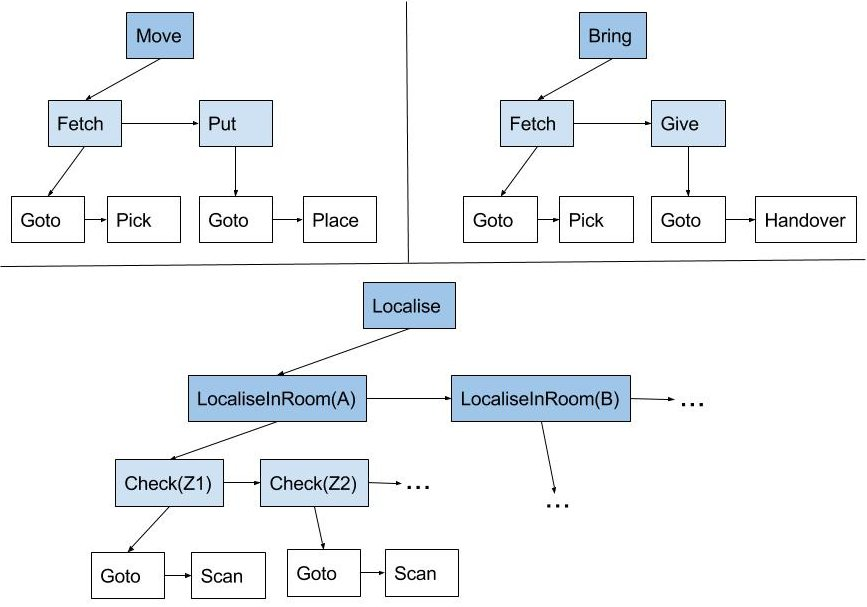
\includegraphics[width=0.99\linewidth]{./img/mardiDom.jpg}
  \caption {Hiérarchie des divers méthodes et actions du domaine de planification définit pour le projet MaRDi.}
  \label{fig:MardiDom}
\end{figure}

Ce domaine ainsi définit permet de mettre au point les plans nécessaires à la résolution des buts susceptibles d'être demandés par l'utilisateur dans le cadre de notre scénario d'interaction homme-robot.


\subsection{Supervision et exécution}
%Parler des différentes règles mises en place

Parmi les buts possibles provenant du dialogue, certains correspondent directement à une des méthodes haut niveau présentée en section \ref{sec:domainehatp}.
Ainsi, si l'homme demande au robot de déplacer un objet \textit{O} vers une zone de manipulation \textit{ZM}, si le robot connaît l'emplacement de \textit{O}, il peut directement planifier pour résoudre la méthode \textit{Move(O, ZM)}. Il en va de même pour les autres méthodes de haut niveau. Cependant, dans le cas où le robot ignore l'emplacement de l'objet certains raisonnements sont nécessaires pour mener à bien la tâche.

Ainsi, lorsque le robot ne connaît pas l'emplacement de l'objet, une façon simple de résoudre le problème est d'appeler d'abord la méthode \textit{Localise} afin de trouver l'emplacement de l'objet, puis effectuer le déplacement demandé le cas échéant. Cependant, le déplacement du robot et les scans successifs des différentes pièces et zones contenues dans ces pièces est coûteux en temps.
Pour réduire au maximum le coût de cette recherche, lorsqu'il doit effectuer un \textit{Localise} le robot va tout d'abord demander si l'humain connaît l'emplacement de l'objet.

Trois cas sont alors possibles.
\begin{itemize}
\item \textbf{Zone de Manipulation}: l'humain peut indiquer un meuble au robot, dans ce cas la supervision pourra directement faire une requête de planification permettant d'effectuer le déplacement de l'objet initialement demandé.

\item \textbf{Pièce}: l'humain peut également indiquer une pièce, dans ce cas le superviseur devra faire une requête de planification \textit{LocaliseInRoom} correspondante. Le plan sera achevé dès que l'objet sera trouvé ou que toutes les zones de manipulations auront leur fait \textit{hasScanned} à \textit{true} pour le robot.

\item \textbf{Emplacement inconnu}: dans le cas où l'homme ignore l'emplacement de l'objet, le superviseur doit alors faire une requête au planificateur avec la méthode \textit{Localise}. Avant d'exécuter ce plan, le superviseur demande l'autorisation à l'homme de pouvoir chercher dans tout l'appartement.
\end{itemize}  


Nous proposons une règle pour prendre en compte l'état de croyance de l'homme concernant la composition des différentes pièces et zones de manipulation pour améliorer la recherche d'objet.
En effet, lorsque l'homme indique une pièce plutôt qu'une zone de manipulation ou lorsqu'il indique qu'il ignore l'emplacement de l'objet, on peut en déduire que l'objet ne se trouve pas dans les pièces ou dans les zones que l'homme a déjà explorées. Lors de l'exécution de la méthode \textit{Localise} le robot va donc explorer en premier lieu les pièces ayant le fait \textit{hasScanned} à \textit{false} pour l'humain et de même pour la méthode \textit{LocaliseInRoom} et les zones de manipulation ayant été explorées par l'homme.


Nous proposons une autre règle pour prendre en compte cette fois-ci l'état de croyance divergente de l'homme et du robot, directement au niveau de la supervision.
Dans le cas où l'homme indique une position erronée de l'objet au robot deux situations peuvent apparaître. (1) Le robot ignore l'emplacement de l'objet mais a déjà scanné la position indiquée par l'homme. Dans ce cas le robot informe l'homme et demande confirmation avant de retourner scanner la zone ou la pièce correspondante (il est possible que le robot ait eu une défaillance au niveau de sa perception lors du scan précédent). (2) Si le robot connaît la position de l'objet et si le superviseur est informé de l'état de croyance divergente de l'homme concernant cet objet, le robot exécutera directement la commande en allant chercher l'objet au bon emplacement. Nous considérons ici qu'il n'est pas nécessaire de contredire l'homme car celui-ci mettra à jour la position de l'objet une fois que le robot aura accompli la tâche demandée.


Enfin, nous avons ajouté une dernière règle permettant de gérer les cas d'échec.
Imaginons que le robot ait exploré toutes les zones mais qu'il n'ait pas trouvé l'objet demandé. Si le robot a connaissance de l'emplacement d'un objet similaire ayant le même type, c'est à dire qu'il a trouvé un autre livre ou un autre DVD étant classé dans la même catégorie (science-fiction, polar, pour enfant...) le robot pourra indiquer à l'homme qu'il n'a pas trouver l'objet demandé mais lui proposer malgré tout l'objet similaire comme alternative à la commande initiale.




\subsection{Expérimentation et résultats}

\subsubsection{Configuration expérimentale}
%Parler des outils utilisés: mocap...
%+ area et locations
Nous avons utilisé la réplique d'appartement du LAAS pour effectuer nos expérimentations. Nous avons simplifié la perception, en utilisant de la capture de mouvement pour suivre les humains. Pour la détection d'objet nous utilisons un logiciel de reconnaissance de tags nommé Viman (déjà présenté en section \ref{sec:chap2expconf}).


Pour effectuer les différents mouvements, nous utilisons un planificateur de mouvement\cite{Sisbot2008} qui commande les actionneurs du robot.
Concernant la navigation, nous utilisons \textit{moveBase} \footnote{http://wiki.ros.org/move\_base}.


Pour le maintien de l'état du monde perçu par le robot et l'évaluation de la situation nous utilisons l'infrastructure TOASTER et sa capacité de gestion des états mentaux présentée dans le chapitre \ref{chapter2}.
Dans cette configuration, nous utilisons les modules \textit{PDG} pour l'agrégation des données d'entrées, le module \textit{area\_manager} pour gérer les différentes zones et la base de données pour accéder aux faits contenus dans les différents modèles.

Nous configurons l'environnement comme présenté à la figure \ref{fig:areasMardi}.
L'environnement contient donc trois pièces qui elles-mêmes contiennent des zones de manipulation.

\begin{figure}[ht!]
 \centering
 \begin{tabular}{cc}
  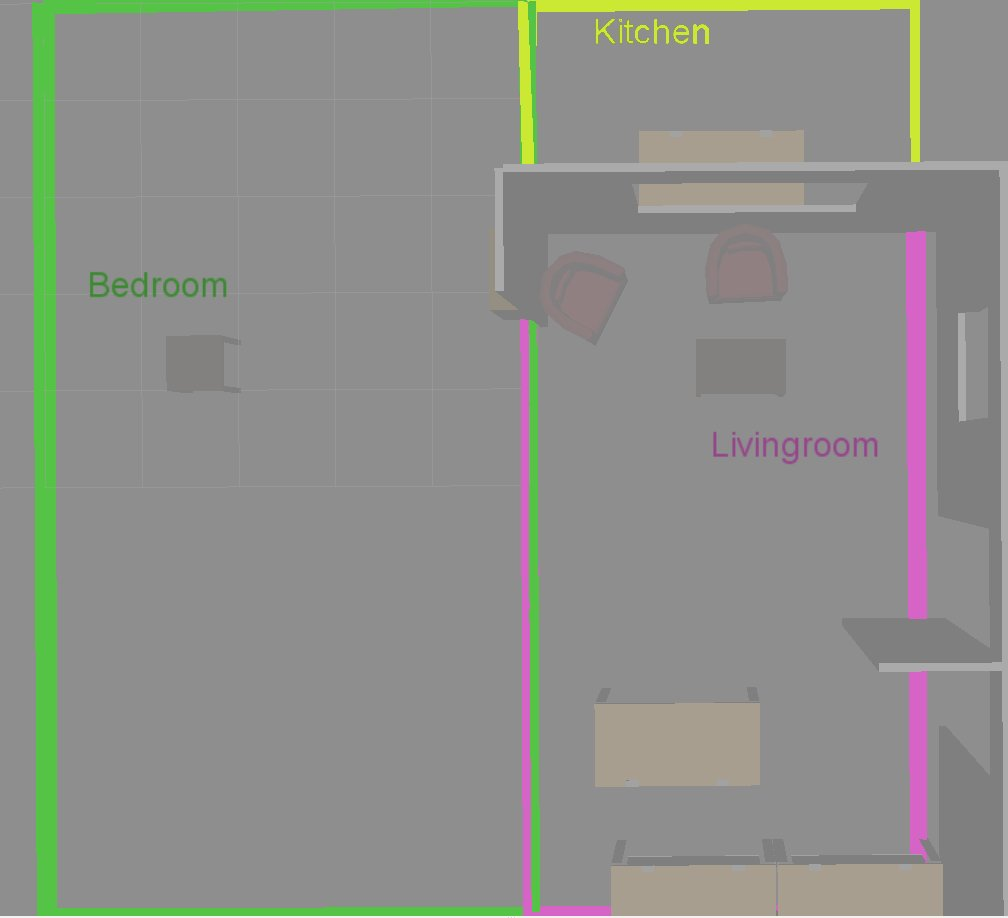
\includegraphics[width=0.49\textwidth]{img/areas.jpg} &
  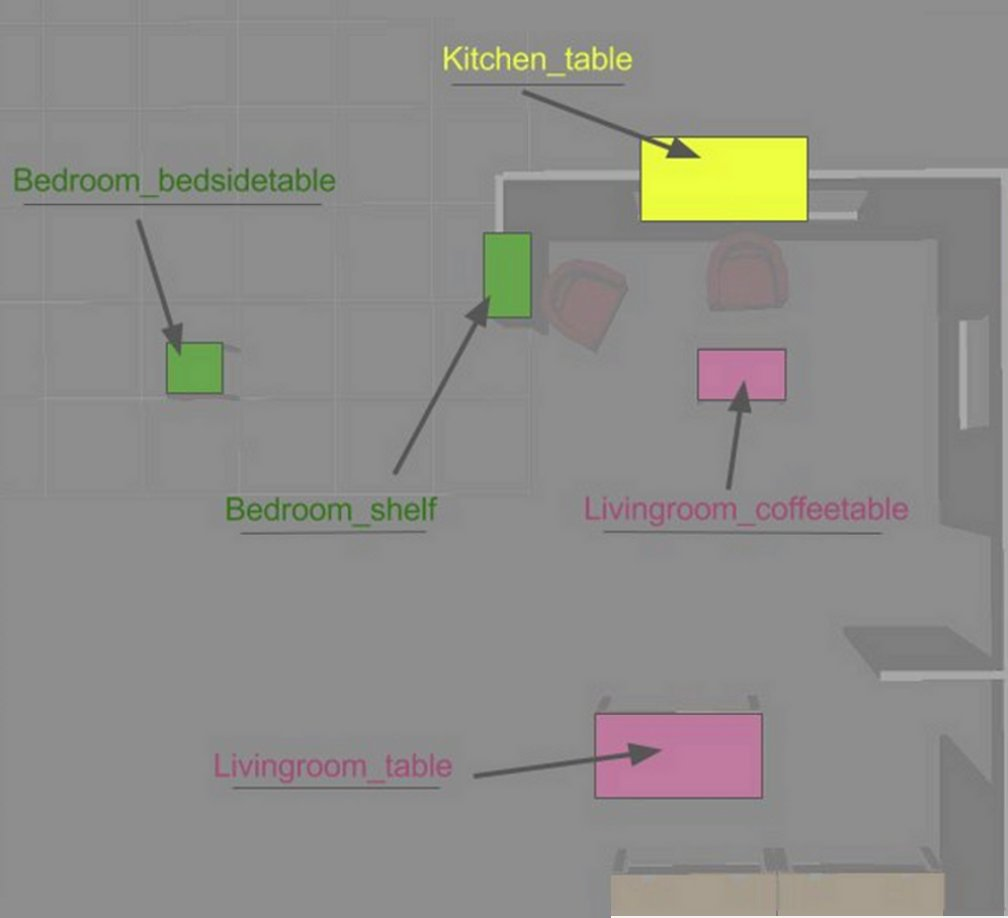
\includegraphics[width=0.49\textwidth]{img/furnitures.jpg}
 \end{tabular}
 \caption{Répartition des différentes pièces (image de gauche) et des différentes zones de manipulation correspondants aux meubles contenus dans ces pièces (image de droite).}
 \label{fig:areasMardi}
%   \vspace{-3pt}
 \end{figure}

\begin{itemize}
\item \textbf{Livingroom}: en rose sur la figure, cette pièce correspond au salon.
Elle contient deux zones de manipulation, la table basse (\textit{Livingroom\_coffetable}) et une autre table (\textit{Livingroom\_table}).

\item \textbf{Bedroom}: en vert sur la figure, cette pièce correspond à la chambre. Elle contient deux zones de manipulation, la table de nuit (\textit{Bedroom\_bedsidetable}) et une étagère (\textit{Bedroom\_shelf}).

\item \textbf{Kitchen}: en jaune sur la figure, cette pièce correspond à la cuisine. Elle contient une table (\textit{Kitchen\_table}).
\end{itemize}

\subsubsection{Expérimentation}


Plusieurs expérimentations ont été réalisées en utilisant cette configuration du système et avec différentes répartitions d'objets et requêtes utilisateur. Nous reportons ici un scénario présentant plusieurs situations intéressantes.

Au début du scénario, le robot n'a pas encore exploré son environnement et ignore donc la position des objets.
Nous démarrons l'expérimentation avec l'homme et le robot se trouvant au niveau de  la table du salon \textit{Livingroom\_table}. Pour induire une croyance divergente, on informe l'homme que le DVD Bilbo Le Hobit \textit{Bilbo} se trouve sur la table de la cuisine.

Les croyances sur l'état du monde perçu par le robot sont représentées ci-dessous.
Tous les faits présents sont vrais. Ils ont été simplifiés pour plus de clarté et le type est indiqué seulement lorsqu'il s'agit d'une information obtenue par le dialogue (les autres ayant été obtenus par perception). Dans le système les faits provenant du dialogue ont un flag pour indiquer la différence avec les autres faits.

%TODO représenté chaque états avec toaster?

\begin{scriptsize}
\begin{verbatim}

          Pr2                                          Human
Pr2   isAt       Livingroom_table         Pr2   isAt        Livingroom_table
Human isAt       Livingroom_table         Human isAt        Livingroom_table
Human hasScanned Livingroom_table         Human hasScanned  Livingroom_table
                                          Bilbo isInRoom    Kitchen  (dialogue)

\end{verbatim}
\end{scriptsize}


L'homme demande alors au robot de lui apporter le DVD du Seigneur des Anneaux (\textit{LOTR}).
Le robot n'ayant pas de connaissance de la position de cet objet, il demande à l'homme s'il la connaît.
L'homme répond alors qu'il se trouve dans la chambre.

Le robot ajoute alors le fait correspondant à son état de croyance et à celui de l'homme:

\begin{scriptsize}
\begin{verbatim}

LOTR isInRoom Bedroom  (dialogue)

\end{verbatim}
\end{scriptsize}


Cette première partie de l'interaction est illustrée par la figure \ref{fig:mardiDemo1}.

\begin{figure}[ht!]
 \centering
  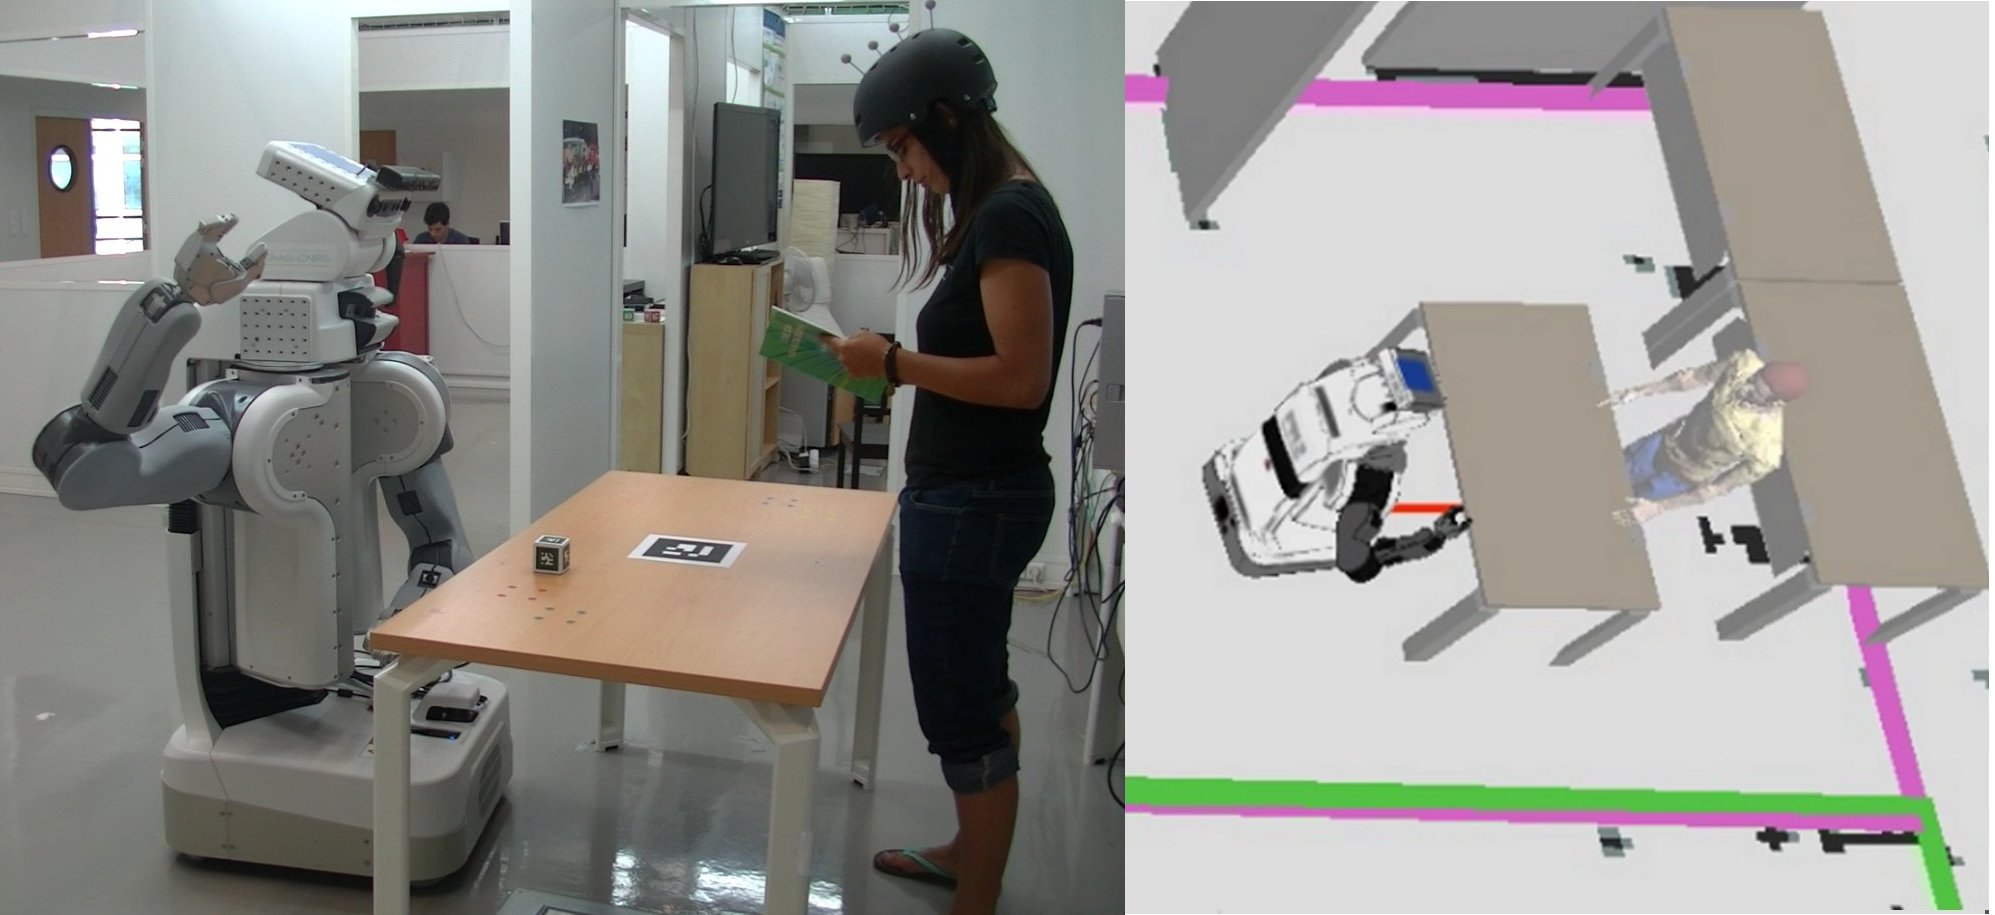
\includegraphics[width=0.99\linewidth]{./img/mardiDemo1b.jpg}
  \caption {L'homme et le robot se trouvent près de la table du salon. À droite la représentation de l'état du monde dans Rviz et à gauche la même scène dans le monde réel.}
  \label{fig:mardiDemo1}
\end{figure}

Suite à cela, la supervision va demander la génération d'un premier plan pour obtenir la localisation exacte de l'objet. Pour cela, le planificateur cherche à trouver comment effectuer la tâche \textit{LocaliseInRoom(Bedroom, LOTR)}.
Pour exécuter cette première tâche, le robot se rend dans la chambre, au niveau de la table de nuit. Il scanne l'emplacement et y trouve le DVD \textit{Bilbo}.

Les faits suivant sont alors ajoutés à son état de croyance.

\begin{scriptsize}
\begin{verbatim}


          Pr2
Bilbo isAt       Bedroom_bedsidetable
Bilbo isInRoom   Bedroom
ROBOT hasScanned Bedroom_bedsidetable

\end{verbatim}
\end{scriptsize}

Le robot n'ayant pas trouvé l'objet recherché, le superviseur poursuit l'exécution du plan. Le robot se dirige donc vers l'étagère de la chambre et scanne l'emplacement.
Il y découvre le DVD du Seigneur des Anneaux.
Le plan de recherche est donc accompli, le robot informe l'homme qu'il a trouvé l'objet en utilisant le \textit{TTS}.
Pendant l'accomplissement de ce plan, l'humain s'est rendu à la table basse du salon.

L'évolution de la situation est présentée par la figure \ref{fig:mardiDemo2} dans laquelle nous montrons l'état du monde tel qu'il est représenté par TOASTER avant et après l'exploration de la chambre.

% \begin{figure}[ht!]
%  \centering
%   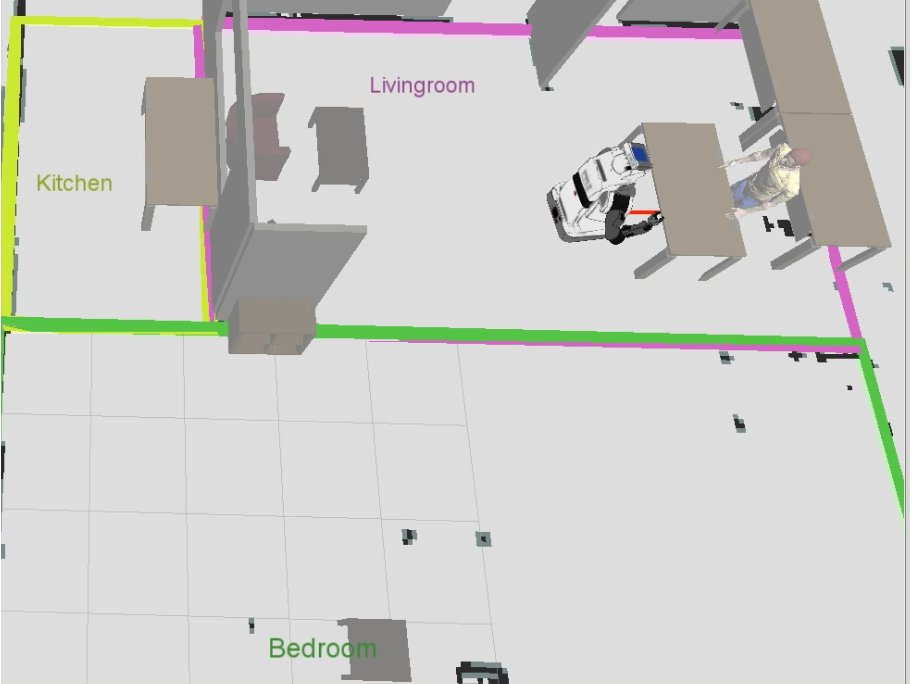
\includegraphics[width=0.99\linewidth]{./img/mardiDemo2b.jpg} &
%    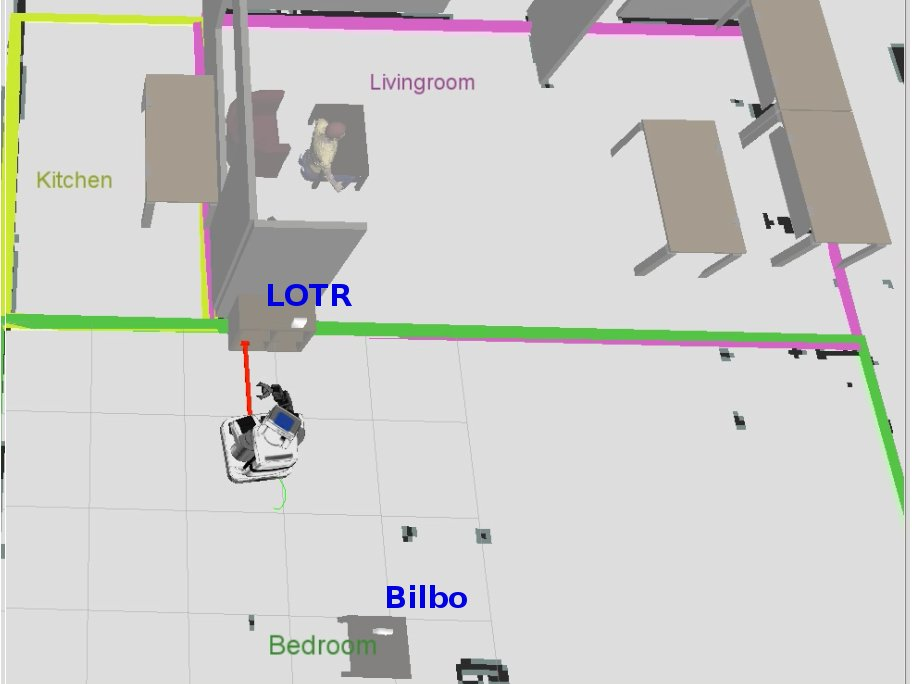
\includegraphics[width=0.99\linewidth]{./img/mardiDemo2c.jpg}
%   \caption {Représentation de l'évolution de l'état du monde après l'exploration de la chambre. L'image de gauche est la visualisation de l'état du monde dans Rviz avant que le robot explore et celle de droite est la même visualisation après l'exploration et la mise à jour de l'état du monde. }
%   \label{fig:mardiDemo2}
% \end{figure}


\begin{figure*}[ht!]
  \begin{center}
    \subfigure[Visualisation dans Rviz de l'état du monde maintenu par TOASTER avant que le robot explore la chambre.]{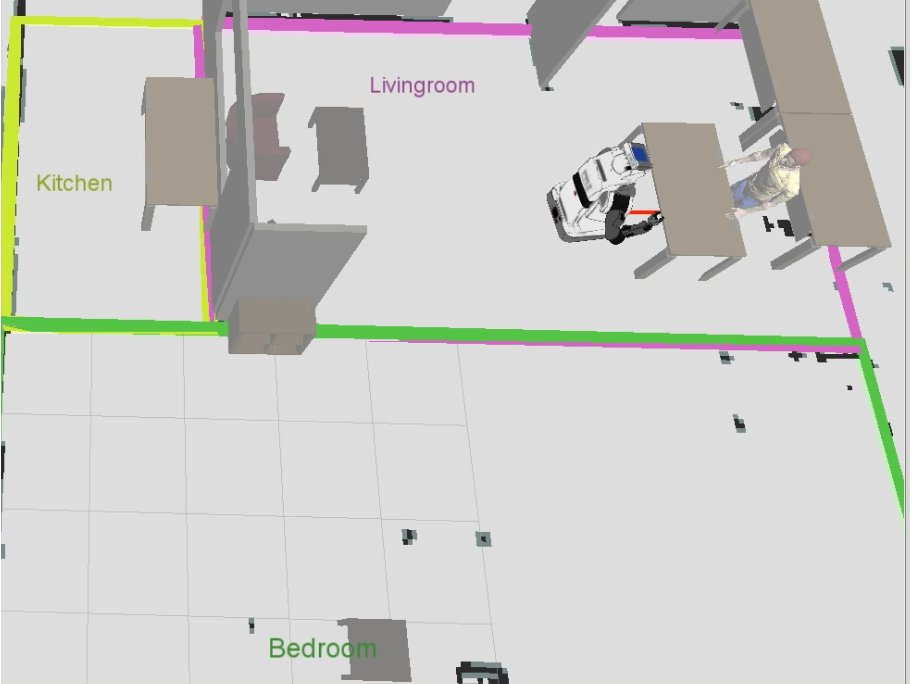
\includegraphics[width=0.83\textwidth]{./img/mardiDemo2b.jpg}}
    \subfigure[Visualisation dans Rviz de l'état du monde maintenu par TOASTER après que le robot explore la chambre.]{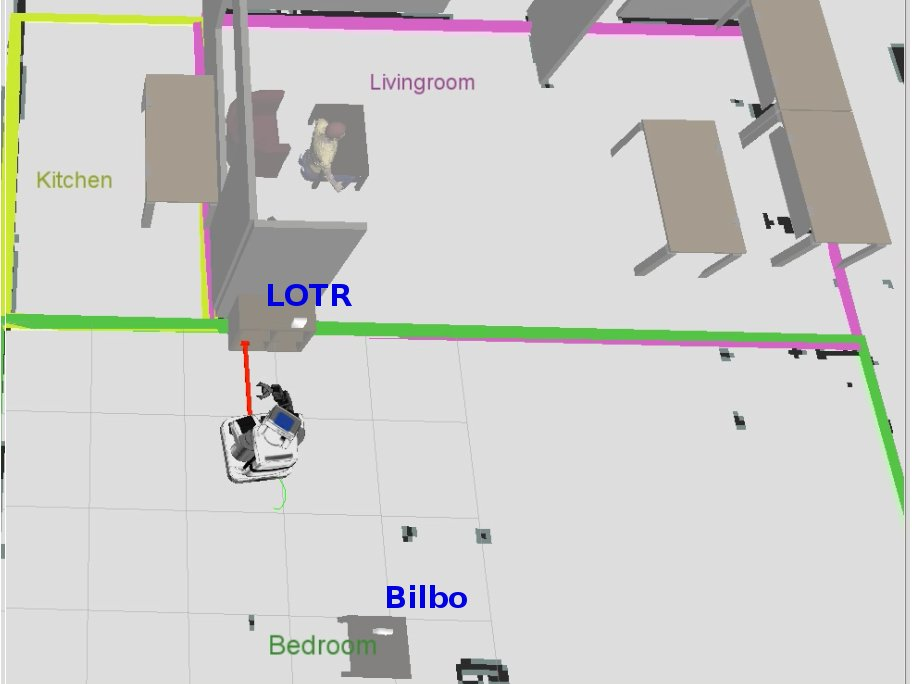
\includegraphics[width=0.83\textwidth]{./img/mardiDemo2c.jpg}}
    \caption {Représentation de l'évolution de l'état du monde après l'exploration de la chambre.}
  \label{fig:mardiDemo2}
  \end{center}
\end{figure*}

Nous présentons les modèles d'état de croyance simplifiés (certains faits isInRoom ont étés enlevés lorsqu'un fait isAt avec le même sujet est présent):

\begin{scriptsize}
\begin{verbatim}


          Pr2                                          Human
Human isAt       Livingroom_coffeetable   Human isAt        Livingroom_coffeetable
Human hasScanned Livingroom               Human hasScanned  Livingroom
Bilbo isAt       Bedroom_bedsidetable     Bilbo isInRoom    Kitchen (dialogue)
LOTR  isAt       Bedroom_shelf            LOTR  isAt        Bedroom_shelf (dialogue)
Pr2   isAt       Bedroom_shelf                
Pr2   hasScanned Bedroom

\end{verbatim}
\end{scriptsize}

La supervision demande alors au planificateur de produire un plan pour résoudre le but courant, à savoir \textit{Bring(LOTR, Human)}.
La supervision va gérer l'exécution pour la génération de mouvement pour attraper l'objet, la navigation vers l'emplacement de l'homme et la génération de mouvement pour transmettre l'objet à l'homme comme illustré par la figure \ref{fig:mardiDemo3}.


\begin{figure}[ht!]
 \centering
  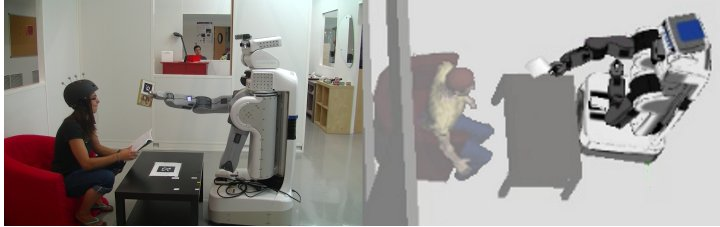
\includegraphics[width=0.99\linewidth]{./img/real2.jpg} 
  \caption {Le robot réalise un "Bring": il va chercher le DVD du Seigneur des Anneaux, le prends puis se déplace vers l'emplacement de l'homme pour lui donner.}
  \label{fig:mardiDemo3}
\end{figure}

Cette première étape permet de montrer comment le robot est capable d'acquérir une information manquante afin d'accomplir une tâche demandée par l'utilisateur. En effet, le robot a demandé à l'homme la position de l'objet, ce qui réduit l'espace de recherche. La réponse de l'homme n'étant pas suffisamment précise pour permettre une exécution directe, la supervision a ordonné au planificateur la production d'un premier plan de recherche d'objet afin d'obtenir l'emplacement précis de l'objet, tout en prenant en compte les indications de l'homme.

Après la réalisation de sa première requête, l'homme fait une autre demande au robot. Il demande cette fois que le robot déplace le livre Cendrillon (\textit{Cinderella}) pour le mettre sur la table basse du salon.
Tout comme l'étape précédente, le robot ne connaissant pas l'emplacement de cet objet, il demande à l'homme s'il sait où trouver ce livre.
L'homme répond qu'il ignore sa position.
Hors, le robot sait que l'homme connaît les éléments qui se trouvent dans le salon (\textit{Human hasScanned  Livingroom}), donc si l'homme ignore la position de cet objet c'est qu'il n'est probablement pas dans le salon. De plus, le robot a déjà exploré la chambre (\textit{Pr2 hasScanned Bedroom}). Le superviseur va donc éliminer ces deux zones de sa recherche et directement demander une génération de plan pour résoudre \textit{LocaliseInRoom(Kitchen Cinderella)}. Cette zone n'ayant pas été indiquée par l'homme le robot demande d'abord l'autorisation avant de se rendre à la cuisine. Ceci permet d'éviter que le robot soit perçu comme intrusif.
Le robot se rend donc à la table de la cuisine, scanne l'emplacement et trouve le livre \textit{Peter\_Pan} mais ne trouve pas \textit{Cinderella}.
Le superviseur n'ayant pas trouvé l'objet et n'ayant plus d'emplacement à scanner, une relâche de contrainte sur l'emplacement est mise en place.
Le superviseur exécute alors le plan \textit{LocaliseInRoom(Livingroom Cinderella)}. On considère ici que, si le robot a cherché partout sans trouver l'objet, il doit alors vérifier qu'il ne se trouve pas aux emplacements observés par l'homme, bien que celui-ci ait affirmé ne pas connaître l'emplacement de l'objet.
Le robot scanne alors les deux emplacements du salon sans succès.
Le robot ayant exploré toutes les zones de l'appartement, il décide alors d'effectuer une relâche de contrainte sur l'objet et propose un objet similaire s'il a connaissance d'un objet similaire présent dans l'environnement.
Ici \textit{Peter\_Pan} est considéré comme un objet similaire car il est du même type (livre) et du même genre (compte pour enfant).
L'humain accepte la proposition, le robot déplace donc \textit{Peter\_Pan} de la cuisine à la table basse du salon, cette action est illustrée par la figure \ref{fig:mardiDemo4}.

\begin{figure}[ht!]
 \centering
  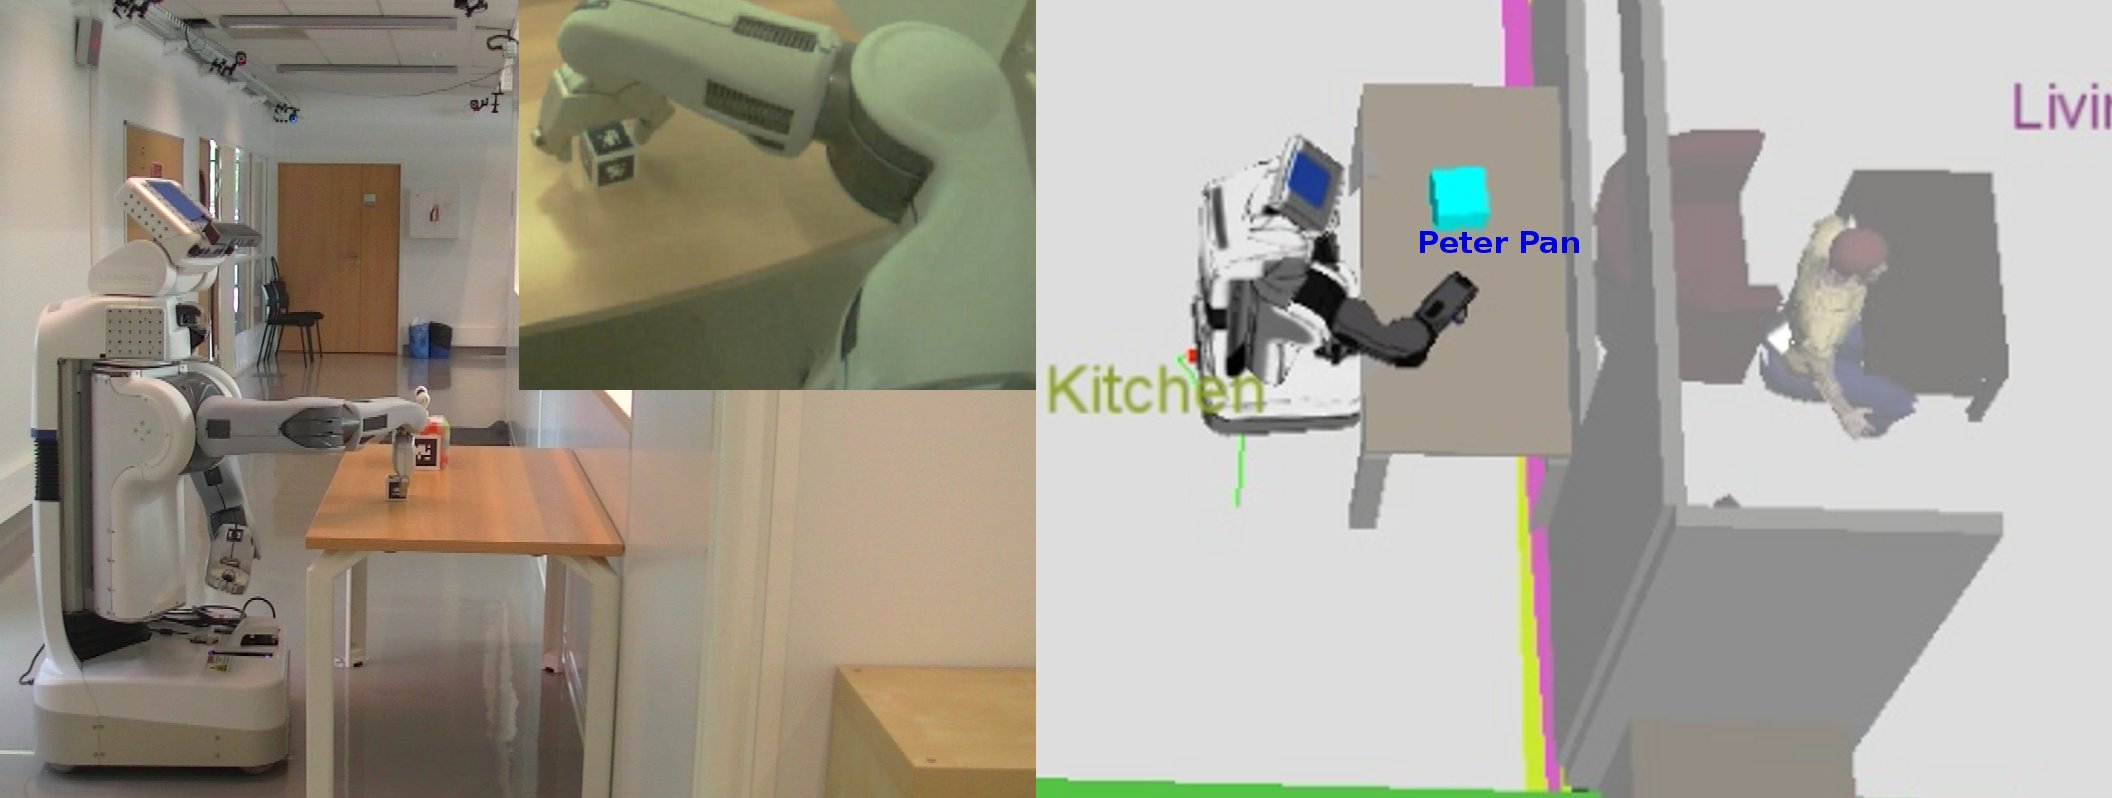
\includegraphics[width=0.99\linewidth]{./img/mardiDemo4.jpg} 
  \caption {Le robot propose de ramener le livre de Peter Pan (ici représenter par un cube pour faciliter la manipulation) car il n'a pas trouver Cendrillon et que ces deux objets sont proches car ils ont le même type (livre) et le même genre (conte pour enfant). L'image de gauche montre le robot attrapant l'objet dans le monde réel et l'image de droite montre la même scène dans Rviz.}
  \label{fig:mardiDemo4}
\end{figure}

Cette deuxième étape illustre la capacité du système à raisonner sur les emplacements possibles en utilisant la prise de perspective perceptuelle pour savoir ce que l'homme a pu observer ou non et pouvoir réduire le champ des possibles concernant l'emplacement de l'objet désiré. Cette expérimentation permet également de montrer comment le robot est capable de relâcher certaines contraintes en cas d'échec de localisation de l'objet désiré, permettant ainsi de proposer une alternative cohérente (proposition d'objet similaire) en cas d'incapacité d'accomplissement du but initial.


Après avoir accompli le déplacement de \textit{Peter\_Pan} les états de croyances des agents sont alors:

\begin{scriptsize}
\begin{verbatim}


          Pr2                                          Human
Pr2   isAt        Livingroom_coffeetable     Pr2   isAt        Livingroom_coffeetable
Human isAt        Livingroom_coffeetable     Human isAt        Livingroom_coffeetable
Human hasScanned  Livingroom                 Human hasScanned  Livingroom
Bilbo isAt        Bedroom_bedsidetable       Bilbo isInRoom    Kitchen (dialogue)
LOTR  isInHand    Human                      LOTR  isInHand    Human 
Peter_Pan isAt    Livingroom_coffeetable     Peter_Pan isAt    Livingroom_coffeetable 
Pr2   hasScanned     Bedroom
Pr2   hasScanned     Livingroom
Pr2   hasScanned     Kitchen

\end{verbatim}
\end{scriptsize}

L'humain demande alors une dernière requête au robot.
Il lui demande d'apporter Bilbo qui se trouve dans la cuisine.
Le robot étant au courant de la croyance erronée de l'homme, la supervision va directement demander au planificateur de résoudre la tâche \textit{Bring(Bilbo, Human)}. Durant l'exécution, le robot utilise son état de croyance et se dirige donc vers la table de nuit pour prendre Bilbo.

Le robot rapporte Bilbo à l'homme et lui tend l'objet.
Le robot est donc parvenu à accomplir la tâche en corrigeant l'énoncé grâce à l'identification de la croyance erronée. De plus, à la fin de l'exécution, comme le robot donne l'objet à l'homme, la croyance erronée a disparu sans que le robot ait eu à en informer l'homme.
Cela donne au robot un aspect efficace et discret en évitant d'informer l'homme lorsque ceci n'est pas nécessaire.

Dans le cas où le robot n'aurait pas trouvé Bilbo sur la table de nuit, il aurait alors mis à jour sa croyance et aurait été voir à l'endroit où l'homme pense que Bilbo se trouve au cas où celui-ci aurait été déplacé sans que le robot en soit informé.

% % génération du plan...
% %%%%%%%%%%%%%%%%%%%%%%%%%%%%%%%%%
% WS: robot isAt Livingroom\_table type=perception
% WS: human isAt Livingroom\_table type=perception
% WS: human scanned Livingroom\_table type=perception

% HS: Bring LOTR\_DVD
% RS: Do you know where?
% HS: Bedroom
% WS: LOTR\_DVD isInRoom Bedroom type=dialogue 

% RA: scan Bedroom\_bedsidetable
% WS: Bilbo isAt Bedroom\_bedsidetable type=perception
% WS: robot scanned Bedroom\_bedsidetable type=perception
% HA: Goto Livingroom\_coffeetable
% WS: human scanned Livingroom\_coffeetable type=perception
% WS: human scanned Livingroom type=perception
% RA: scan Bedroom\_shelf
% WS: LOTR isAt shelf type=perception
% WS: robot scanned Bedroom\_bedsidetable type=perception 
% RS: I found it
% RA: bring LOTR to human
% RS: Here it is

% %%%%%%%%%%%%%%%%%%%%%%%%%%%%%%%%%%%%%%%
% WS: robot isAt Livingroom\_coffeetable type=perception
% WS: human isAt Livingroom\_coffeetable type=perception
% WS: human scanned Livingroom\_coffeetable type=perception
% WS: human scanned Livingroom\_table type=perception
% WS: human scanned Livingroom type=perception
% WS: robot scanned Bedroom\_bedsidetable type=perception
% WS: robot scanned Bedroom\_shelf type=perception
% WS: robot scanned Bedroom type=perception
% WS: LOTR isInHand human type=perception
% WS: Bilbo isAt Bedroom\_bedsidetable type=perception

% HS: Thx, now move the book Cinderella to the coffee\_table
% RS: Do you know where it is?
% HS: No
% RS: Can I look in the appartement?
% HS: Yes
% RA: LocaliseInArea kitchen
% WS: robot scanned kitchen\_table type=perception
% WS: PeterPan isAt Kitchen\_table type=perception
% % Object not found => robot release counstraint on human scanned
% RA: LocaliseInArea Livingroom
% % Object not found, appartement scanned => robot release counstraint on object
% RS: I didn't find Cinderella but I found Peter Pan. Should I bring it to you?
% HS: Yes please
% RS: ok
% RA: Move(Peter Pan, coffee\_table)
% RS: done

% %%%%%%%%%%%%%%%%%%%%%%%%%%%%%%%%%%%
% WS: robot isAt Livingroom\_coffeetable type=perception
% WS: human isAt Livingroom\_coffeetable type=perception
% WS: human scanned Livingroom\_coffeetable type=perception
% WS: human scanned Livingroom\_table type=perception
% WS: human scanned Livingroom type=perception
% WS: robot scanned Bedroom\_bedsidetable type=perception
% WS: robot scanned Bedroom\_shelf type=perception
% WS: robot scanned Bedroom type=perception
% WS: robot scanned Kitchen\_table type=perception
% WS: robot scanned Kitchen type=perception
% WS: LOTR isInHand human type=perception
% WS: PeterPan isAt Livingroom\_coffeetable type=perception
% WS: Bilbo isAt Bedroom\_bedsidetable type=perception


% % Divergent belief
% HWS: Bilbo isAtkitchen\_table type=dialogue

% HS: Bring Bilbo from Kitchen
% RS: Ok
% RA: Bring Bilbo (from bedsidetable)

\section{Conclusion}
\label{sec:chap3conclusion}
Dans ce chapitre nous avons présenté notre contribution au projet MaRDi qui vise à utiliser les informations contextuelles pour améliorer les performances du dialogue en tenant compte de l'aspect situé de celui-ci durant une interaction homme-robot.

Pour réaliser cela, les données contextuelles générées par notre infrastructure d'évaluation de la situation sont utilisées à différents niveaux de l'interaction et par différents modules impliqués dans l'architecture.

Bien que cela n'ait pas été intégré à la version finale, les données contextuelles de bas niveau (position, configuration), peuvent être utilisées comme données d'entrée. L'analyse de la gestuelle de l'homme permet une entrée multimodale du système afin de saisir la référence faite à un objet pointé. Ces données contextuelles de bas niveau sont également utilisées au niveau de la fission pour commander au \textit{TTS} de générer une voix adaptée à la situation (voix portée, voix normale) et pour décider d'ajouter ou non de la gestuelle à la parole (si le robot est proche et visible par l'homme).

La représentation symbolique de l'environnement issue de raisonnements géométriques rend également possible l'identification des référents utilisés par l'homme dans sa communication verbale (par exemple, "Le livre qui est sur la table?" peut être identifié en recherchant tous les livres étant le sujet du fait \textit{? isOn Table}).

Nous avons également montré comment, en partant du principe que l'homme fait des demandes logiques, il est possible d'utiliser les informations disponibles en terme de prise de perspective perceptuelle pour réduire la liste des candidats pour identifier un objet désigné par l'homme.
Ainsi, grâce à des règles simples (l'homme ne cherche pas un objet qui lui est visible et ne demande pas de ramener un objet qui lui est atteignable) le mécanisme de fusion est rendu plus efficace.

De même, nous avons montré comment la prise de perspective conceptuelle et notamment l'identification de croyance divergente permet d'améliorer le gestionnaire de dialogue en ajoutant un état et une action possible afin de permettre au système de décider de la politique à adopter en prenant en compte cette croyance divergente lors de l'interprétation de la commande utilisateur.
Cette amélioration a pu être testée en utilisant un simulateur robotique afin de faire interagir des utilisateurs avec le système et a confirmé une amélioration tant au niveau de l'efficacité que du taux de réussite concernant la résolution de tâches impliquant une croyance divergente de l'homme.

Enfin, nous avons implémenté un système de supervision basé sur des règles pour permettre au robot d'acquérir une information manquante (la position d'un objet) en utilisant un raisonnement sur sa propre connaissance et sur celle de l'humain.
Nous avons également montré comment il est possible au robot de s'adapter en proposant une alternative cohérente dans le cas où la requête utilisateur ne pouvait être satisfaite.


Nous avons donc montré à quel point l'interprétation des données contextuelles, du plus bas niveau (position, distance...) au plus haut niveau (prise de perspective) sont essentielles à tous les niveaux de l'architecture pour permettre un dialogue situé efficace et de qualité.

Cependant, cette architecture et cette implémentation peuvent être améliorées en utilisant par exemple les aspects temporels présents dans la base de données (présentée en section \ref{sec:dbt}) et également la mémoire des agents (présentée en section \ref{sec:dbPt}). Cela permettrait par exemple de pouvoir répondre à des requête utilisateur du type "Qui a pris le livre qui était sur la table" en interprétant dans la mémoire d'état de croyance de l'interlocuteur afin d'identifier l'objet dont il parle et d'utiliser la table des événements  \textit{EVENT\_TBL} afin de trouver qui a pris l'objet.

L'interaction considérée prévoit que l'homme est globalement passif durant l'exécution de plan. Un des moyens d'aller plus loin dans cette étude serait de faire collaborer l'homme avec le robot comme pour l'étude qui sera présentée au chapitre \ref{chapter5}.

De plus, les études utilisateur effectuées jusque là ont été faites uniquement sur simulateur avec une exécution simulée. Il serait intéressant d'avoir des retours sur la perception du système dans un environnement réel. 


%TODO
% In this paper, we described how a user belief realtime tracking framework can be used along with a multimodal POMDP-based dialogue management. The evaluation of the proposed method with real users confirms that this additional information helps to achieve more efficient and natural task planning (and does not harm handling of normal situations). 
% %In the present work, for practical reasons, the interactions took place in a simulated 3D environment. However, the spatial reasoning framework responsible for the agent belief management is already operational for on-board interaction. 
% Our next step will be to integrate the multimodal dialogue system on the robot and carry out evaluations in real setting to uphold our claims in an fully realistic configuration.

% \subsection{Représentation Symbolique de l'État du Monde}
% Robot -> x y z
% Humain -> sur, à côté de ...

% \subsection{Prise de Perspective Perceptuelle}
% disambigüe
% \subsection{Prise de Perspective Conceptuelle}

% \section{Implémentation}
% Archi MaRDi

% \section{Résultats expérimentaux}
% MORSE
% papier IWSDS




\ifdefined\included
\else
\bibliographystyle{acm}
\bibliography{These}
\end{document}
\fi
